\documentclass[11pt]{article}

% Paquetes
%===================================================================================================

% Establecemos los márgenes
\usepackage[a4paper, margin=1in]{geometry}

% Separacion entre parrafos
\setlength{\parskip}{1em}

% Paquete para incluir codigo
\usepackage{listings}

% Paquete para incluir imagenes
\usepackage{graphicx}
\graphicspath{ {./images/} }

% Para fijar las imagenes en la posicion deseada
\usepackage{float}

% Para que el codigo acepte caracteres en utf8
\lstset{literate=
  {á}{{\'a}}1 {é}{{\'e}}1 {í}{{\'i}}1 {ó}{{\'o}}1 {ú}{{\'u}}1
  {Á}{{\'A}}1 {É}{{\'E}}1 {Í}{{\'I}}1 {Ó}{{\'O}}1 {Ú}{{\'U}}1
  {à}{{\`a}}1 {è}{{\`e}}1 {ì}{{\`i}}1 {ò}{{\`o}}1 {ù}{{\`u}}1
  {À}{{\`A}}1 {È}{{\'E}}1 {Ì}{{\`I}}1 {Ò}{{\`O}}1 {Ù}{{\`U}}1
  {ä}{{\"a}}1 {ë}{{\"e}}1 {ï}{{\"i}}1 {ö}{{\"o}}1 {ü}{{\"u}}1
  {Ä}{{\"A}}1 {Ë}{{\"E}}1 {Ï}{{\"I}}1 {Ö}{{\"O}}1 {Ü}{{\"U}}1
  {â}{{\^a}}1 {ê}{{\^e}}1 {î}{{\^i}}1 {ô}{{\^o}}1 {û}{{\^u}}1
  {Â}{{\^A}}1 {Ê}{{\^E}}1 {Î}{{\^I}}1 {Ô}{{\^O}}1 {Û}{{\^U}}1
  {ã}{{\~a}}1 {ẽ}{{\~e}}1 {ĩ}{{\~i}}1 {õ}{{\~o}}1 {ũ}{{\~u}}1
  {Ã}{{\~A}}1 {Ẽ}{{\~E}}1 {Ĩ}{{\~I}}1 {Õ}{{\~O}}1 {Ũ}{{\~U}}1
  {œ}{{\oe}}1 {Œ}{{\OE}}1 {æ}{{\ae}}1 {Æ}{{\AE}}1 {ß}{{\ss}}1
  {ű}{{\H{u}}}1 {Ű}{{\H{U}}}1 {ő}{{\H{o}}}1 {Ő}{{\H{O}}}1
  {ç}{{\c c}}1 {Ç}{{\c C}}1 {ø}{{\o}}1 {å}{{\r a}}1 {Å}{{\r A}}1
  {€}{{\euro}}1 {£}{{\pounds}}1 {«}{{\guillemotleft}}1
  {»}{{\guillemotright}}1 {ñ}{{\~n}}1 {Ñ}{{\~N}}1 {¿}{{?`}}1 {¡}{{!`}}1
}

% Para que no se salgan las lineas de codigo
% Para fijar una fuente que resalte
\lstset{breaklines=true, basicstyle=\ttfamily}

% Para que los metadatos que escribe latex esten en español
\usepackage[spanish]{babel}
\decimalpoint % Para que no se cambie el punto a la coma

% Para la bibliografia
% Sin esto, los enlaces de la bibliografia dan un error de compilacion
\usepackage{url}

% Para que se puedan clicar los enlaces
\usepackage{hyperref}

% Para mostrar graficas de dos imagenes, cada una con su caption, y con un caption comun
\usepackage{subcaption}

% Simbolo de los numeros reales
\usepackage{amssymb}

% Para que los codigos tengan una fuente distinta
\usepackage{courier}

\lstdefinestyle{CustomStyle}{
  language=Python,
  numbers=left,
  stepnumber=1,
  numbersep=10pt,
  tabsize=4,
  showspaces=false,
  showstringspaces=false
  basicstyle=\tiny\ttfamily,
}

% Para referenciar secciones usando el nombre de las secciones
\usepackage{nameref}

% Para enumerados dentro de enumerados
\usepackage{enumitem}

% Para mejores tablas
\usepackage{tabularx}

% Para poder tener el mismo identificador en dos tablas separadas
\usepackage{caption}

% Mostrar la página de las referencias en el indice del documento
\usepackage[nottoc,numbib]{tocbibind}

% Para mostrar las matrices
\usepackage{amsmath}

% Funciones de latex personalizadas
%===================================================================================================

% Para realizar las citas de forma corta
\newcommand{\customcite}[1]{\emph{``\ref{#1}. \nameref{#1}''}}

% Metadatos del documento
%===================================================================================================
\title{
    {Prácticas Inteligencia de Negocio}
}

\author{
    {Sergio Quijano Rey - 72103503k}\\
    {sergioquijano@correo.ugr.es} \\
    {5º Doble Grado Ingeniería Informática y Matemáticas} \\
    {Grupo de prácticas 1}
}

\date{\today}

% Separacion entre parrafos
\setlength{\parskip}{1em}

% Contenido del documento
%===================================================================================================
\begin{document}

% Portada del documento
\maketitle
\pagebreak

% Indice de contenidos
\tableofcontents

% Lista de figuras
% Uso el addtocontents para que no se muestre la seccion de indice de figuras en el indice inicial

\addtocontents{toc}{\setcounter{tocdepth}{-10}}
\listoffigures
\addtocontents{toc}{\setcounter{tocdepth}{2}}

\pagebreak

\section{Introducción}

En esta sección hablaremos de cada uno de los problemas abordados, tratando las particularidades de cada caso y algunas consideraciones en base a estas peculiaridades tratadas.

\subsection{Información general}

En todas las partes en las que necesitemos usar números aleatorios, usaremos la semilla $123456789$ para poder reproducir bajo las mismas condiciones los experimentos y para que las comparaciones entre los distintos algoritmos sean lo más justas posible. En los siguientes sub-apartados, introduciremos los distintos problemas a tratar, sus características y problemas que puedan plantear.

En todos los \emph{datasets} hemos usado la misma estructura jerárquica apoyándonos en los metanodos de \lstinline{KNIME}. Esta estructura busca una mayor limpieza en el \emph{``código''}. Dicha estructura se va a ir vislumbrando a lo largo de las secciones de estas memorias, donde incluiremos capturas de pantalla de los distintos \emph{workflows} desarrollados.

\pagebreak

\subsection{\emph{Heart Failure Prediction}} \label{intro_dataset01:seccion}

En primer lugar, la fuente original del \emph{dataset} se puede encontrar en \cite{heart_disease_dataset:online}. Aunque podemos estar trabajando con un \emph{dataset} ligeramente modificado por los profesores de la asignatura, al igual que con el resto de \emph{datasets} que estudiaremos en esta práctica.

En la propia página de la que se obtiene el dataset \cite{heart_disease_dataset:online}, se especifica que la tarea a resolver para este \emph{dataset} es \emph{``Create a model to assess the likelihood of a possible heart disease event. This can be used to help hospitals in assessing the severity of patients with cardiovascular diseases''}. Es decir, nuestra tarea es generar un modelo de clasificación para predecir, con los datos de entrada dados, si un paciente puede desarrollar algún problema de tipo cardiaco.

En el siguiente apartado, pasamos a comentar las particularidades de este \emph{dataset}, información que hemos extraído con el análisis exploratorio hecho en \lstinline{KNIME}:

\subsubsection{Análisis Exploratorio de los Datos}

Realizamos un pequeño \emph{Análisis Exploratorio Inicial} (\emph{EDA}) de los datos usando las herramientas que nos proporciona \lstinline{KNIME}.

Como ya comentábamos en \customcite{intro_dataset01:seccion}, buscamos predecir si una persona tendrá problemas de tipo cardiaco. Por tanto, la variable de salida con la que vamos a trabajar es \lstinline{HeartDisease}. Consideraremos, por su mayor relevancia, como clase positiva, a la clase $1$.

Lo primero que vemos es que tenemos $12$ variables ($11$ variables de entrada más la variable de salida) y $918$ filas (y por tanto, $918$ ejemplos).

El \emph{workflow} de mayor nivel, para este primer \emph{dataset}, se muestra en la siguiente figura:

\begin{figure}[H]
    \centering
    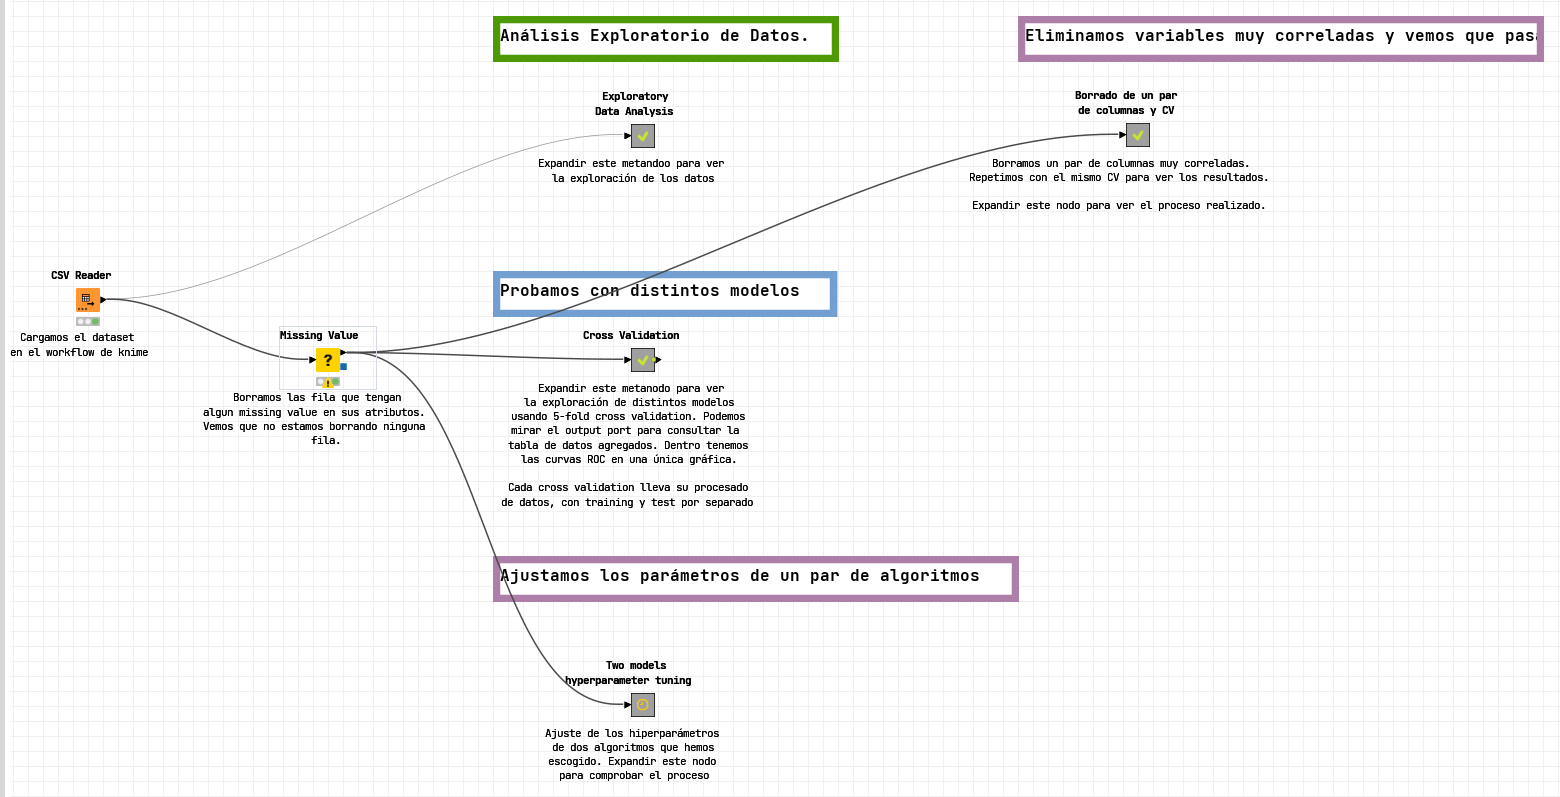
\includegraphics[width = 0.8 \textwidth]{workflow_dataset01}
    \caption{\emph{Workflow} de más alto nivel para el primer \emph{dataset}}
    \label{workflow_general:imagen}
\end{figure}

La parte que ahora nos interesa es la de Análisis Exploratorio de Datos, que mostramos en la siguiente figura:

\begin{figure}[H]
    \centering
    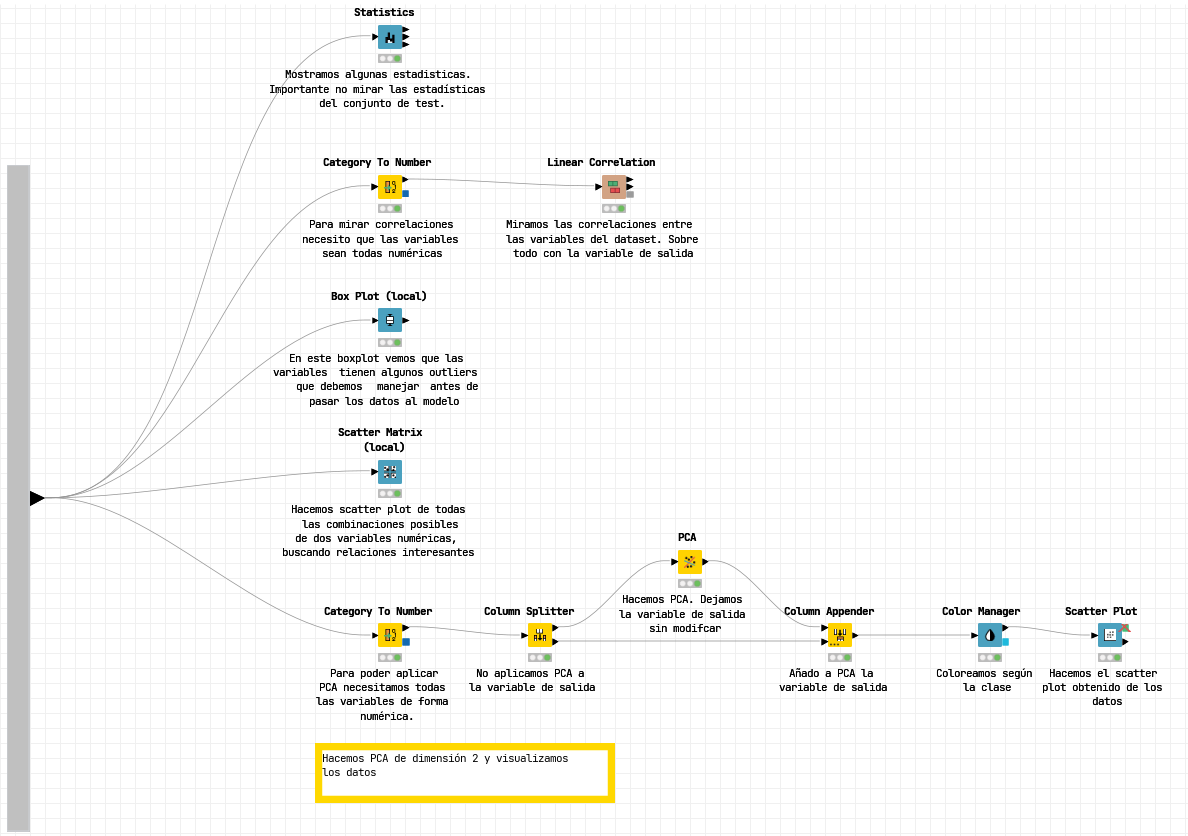
\includegraphics[width = 0.8 \textwidth]{eda_workflow_dataset01}
    \caption{\emph{Workflow} de Análisis Exploratorio de Datos para el primer \emph{dataset}}
\end{figure}

Empezamos con el nodo de estadísticas, que nos muestra que tenemos $410$ ejemplos para la clase de salida $0$ y $508$ para la clase $1$. Por tanto tenemos un ligero desbalanceo ($44.66\%$ para la clase $0$ y $55.34\%$ para la clase $1$), pero en este \emph{dataset} no vamos a tratar dicho desbalanceo. En futuros \emph{datasets} nos vamos a encontrar con clases mucho más desbalanceadas.

Dentro del anterior nodo vemos las distribuciones de las otras variables con las que trabajamos, sin llegar a conclusiones de gran relevancia, salvo razonamientos del tipo hay una característica que predomina en un valor sobre el otro valor en la población, o la población tiene una distribución de la variable normal o con cierta asimetría hacia un lado. Ejemplo de característica que predomina se muestra en la siguiente figura:

\begin{figure}[H]
    \centering
    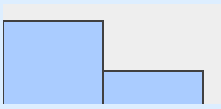
\includegraphics[width = 0.8 \textwidth]{dataset01_var_predominante}
    \caption{Distribución de la variable sexo. A izquierda, los hombres. A la derecha, las mujeres. Es claro que tenemos muchos más hombres que mujeres en nuestra población.}
    \label{variable_predominante:imagen}
\end{figure}

Esta información puede ser utilizada de forma experta en nuestros sistemas automáticos. Sin embargo, por una cuestión de tiempo, no realizamos un ajuste tan a fondo de los modelos que vamos a generar (sobre todo teniendo en cuenta que practicar esto para los cuatro \emph{datasets} es inviable. En otros \emph{datasets} realizaremos una selección de variables usando otras técnicas).

Ejemplo de una distribución con cierta asimetría se muestra a continuación:

\begin{figure}[H]
    \centering
    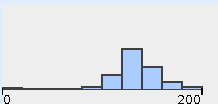
\includegraphics[width = 0.6 \textwidth]{dataset01_var_asimetrica}
    \caption{Distribución de la variable \lstinline{RestingBP}. Podemos ver claramente cómo se acumula más hacia la derecha.}
\end{figure}

De nuevo, esta información es interesante para plantear los modelos de aprendizaje automático de una forma mucho más concienzuda, pero por la extensión de la práctica en técnicas y aspectos a tener en cuenta, no entramos en detalle en este aspecto.

Lo siguiente que hacemos en el Análisis Exploratorio de Datos es mostrar la matriz de correlaciones lineales, que presentamos a continuación:

\begin{figure}[H]
    \centering
    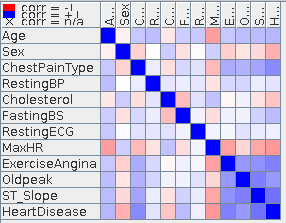
\includegraphics[width = 0.8 \textwidth]{dataset01_correlaciones}
    \caption{Matriz de correlaciones lineales. Un color azul significa correlación lineal positiva, y un color rojo significa correlación lineal negativa.}
    \label{dataset01_correlaciones:imagen}
\end{figure}

Vemos algunas variables correladas. Las más interesantes son el grupo que forman las variables \lstinline{MaxHR} \lstinline{ExerciseAngina}, \lstinline{Oldpeak}, \lstinline{ST_Slope} y la variable de salida \lstinline{HeartDisease}. Sabiendo que estas variables están muy correladas, y que una de ellas es la variable de salida, podríamos probar a construir los modelos predictivos en base a este grupo de variables. Por tanto, estamos justificando el interés de que, más adelante, probemos a eliminar ciertas filas empleando esta matriz de correlaciones, y ver cómo afecta esto al rendimiento de nuestros modelos.

Mostramos ahora los \emph{boxplots} de algunas variables, para ver que tenemos ciertos valores \emph{outliers}:

\begin{figure}[H]
    \centering
    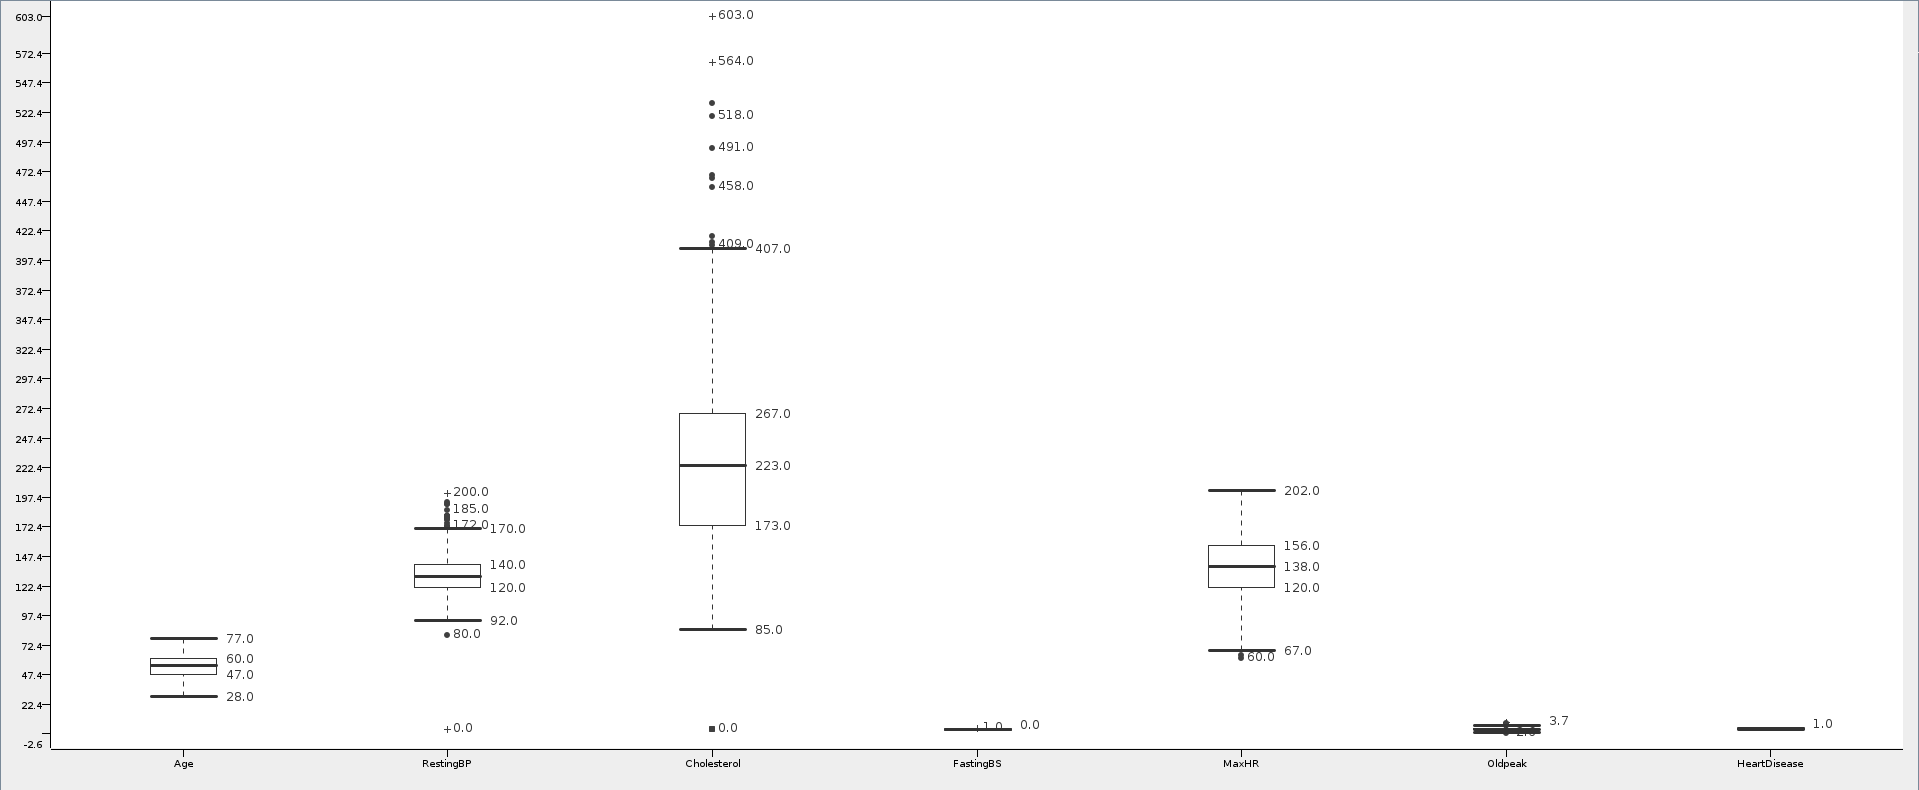
\includegraphics[width = 0.9 \textwidth]{dataset01_boxplots}
    \caption{\emph{Boxplots} de algunas de las variables con las que trabajamos. Queda claro que tenemos \emph{outliers} (sabiendo que están alejados de la media más de 3 veces la desviación típica). Por tanto, tendremos que tratar de alguna forma estos \emph{outliers}}
\end{figure}

También hacemos \emph{plots} de todas las combinaciones posibles entre dos variables, obteniendo la siguiente gráfica:

\begin{figure}[H]
    \centering
    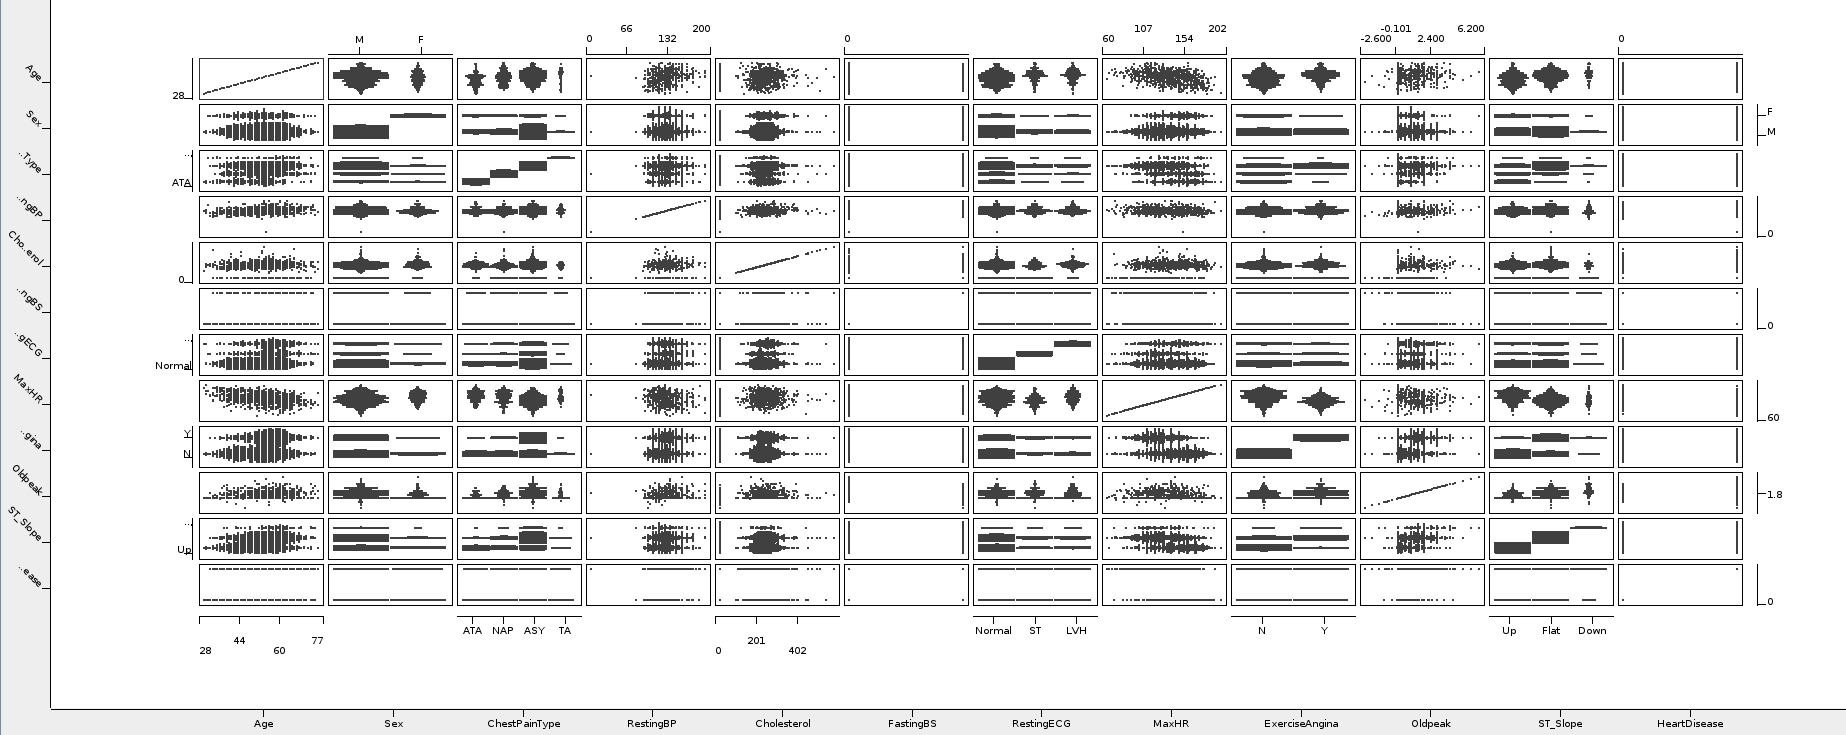
\includegraphics[width = 0.9 \textwidth]{dataset01_combinaciones}
    \caption{Gráficas de todas las posibles combinaciones de dos variables de nuestro dataset}
\end{figure}

De nuevo, como ya comentábamos para \customcite{variable_predominante:imagen}, podemos extraer de esta gráfica algunas conclusiones sobre la distribución de las variables y algunas relaciones que, por simpleza del problema y por falta de tiempo, no vamos a incluir en nuestro modelo.

En último lugar, probamos a aplicar \emph{PCA} al \emph{dataset} para obtener solo dos variables de entrada junto con la variable de salida, buscando sacar alguna información de alto nivel del problema. Esta técnica busca transformar el conjunto de datos con nuevas variables, de modo que estas variables no estén correlacionadas entre sí manteniendo el máximo posible de la varianza del conjunto de datos original. Este procedimiento se apoya en la descomposición en valores propios de la matriz de covarianzas \cite{pca:online}. Mostramos las dos variables obtenidas usando \emph{PCA}, coloreando cada punto del plano $2D$ según a la clase a la que pertenecen:

\begin{figure}[H]
    \centering
    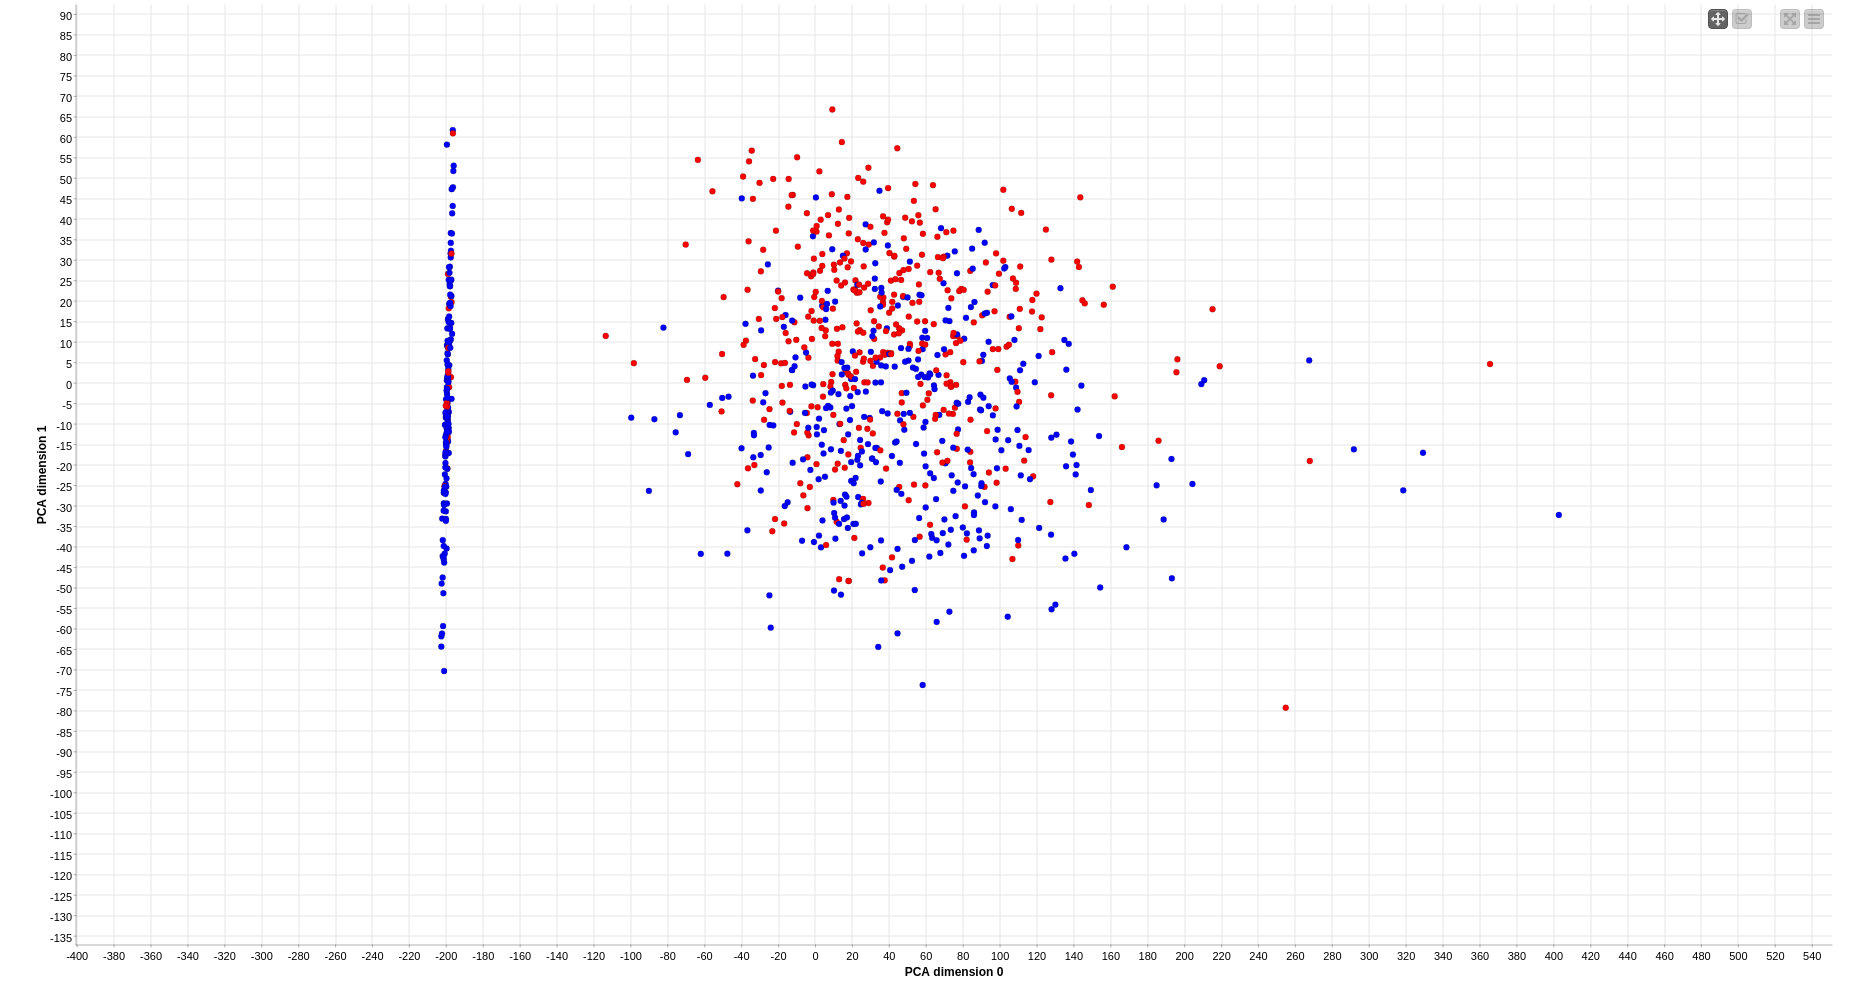
\includegraphics[width = 0.9 \textwidth]{dataset01_pca}
    \caption{Resultado de aplicar \emph{PCA} en dos dimensiones, coloreando cada punto según la clase a la que pertenecen}
\end{figure}

Los resultados obtenidos no nos invitan a usar \emph{PCA} para usarlo como base a modelos de aprendizaje automático. Sin embargo es interesante que se ha obtenido una línea a la izquierda con clara predominancia de la clase representada por el color azul, mientras que a la derecha se obtiene un \emph{clúster} ligeramente circular donde los datos de las dos clases están mezclados sin un patrón claro (quizás la clase roja tiene mayor predominancia en la parte superior). Estamos seguros de que aplicando \emph{PCA} con dimensiones mayores obtendríamos un buen \emph{performance} en los modelos de aprendizaje automático. Pero como para otros \emph{datasets} es más interesante aplicar esta técnica, lo dejamos para más adelante.

En último lugar, tratamos los \textbf{\emph{missing values}}. En el \emph{workflow} de más alto nivel, hacemos una primera aproximación al tratamiento de los \emph{missing values}. Tratamos de borrar todas las filas que contengan \emph{missing values}, pero no borramos ninguna fila. En un principio pensamos que no tenemos \emph{missing values} en este \emph{dataset}. Sin embargo, explorando la colección de datos comprobamos el siguiente hecho: la variable \lstinline{Cholesterol} contiene \emph{missing values} codificados con el valor $0$. Para tratar estos \emph{missing values}, en \emph{Cross Validation} los marcaremos como tal, y los trataremos convenientemente en cada nodo de validación (para evitar hacer \emph{data snooping}). Entraremos en detalles más adelante.

El nodo que usamos para realizar esta comprobación sobre los \emph{missing values} se muestra en el \emph{workflow} general que aparece en \customcite{workflow_general:imagen}.

\pagebreak

\subsection{Mobile Price Classification}

En primer lugar, la fuente original del \emph{dataset} se puede encontrar en \cite{mobile_dataset:online}. De nuevo, podemos estar trabajando con un dataset ligeramente modificado por los profesores de la asignatura.

Según \cite{mobile_dataset:online}, la tarea a resolver es: \emph{``In this problem you do not have to predict actual price but a price range indicating how high the price is''} para un cliente que quiere hacer la competencia a grandes compañías fabricantes de dispositivos móviles. Por lo tanto, tenemos que generar modelos que sean capaces de predecir dicho rango de precios.

En el siguiente apartado pasamos a comentar las particularidades de este \emph{dataset}, particularidades que hemos extraído del \emph{EDA} realizado sobre el conjunto de datos.


\subsubsection{Análisis Exploratorio de los datos} \label{dataset02_eda:seccion}

Estamos usando el mismo \emph{workflow} para el \emph{EDA} que en el \emph{dataset} anterior, así que no mostramos las capturas de los \emph{workflows} de nuevo, sino que mostramos directamente los resultados, que es lo verdaderamente novedoso respecto al \emph{dataset} anterior.

El primer problema que nos encontramos es que tenemos cuatro clases, en vez de dos clases. Por tanto, ya no estamos en un problema de clasificación binaria. Comentaremos más adelante, en \customcite{mobile_price_cross_validation:seccion}, cómo hemos trabajado este problema. Ahora mismo, en el \emph{EDA}, este paso a clasificación multiclase no nos supone ningún problema.

La primera diferencia en los \emph{workflows} con el \emph{dataset} anterior es que estamos haciendo un \emph{rename} de la clase positiva (que en nuestro caso consideramos la clase con valor 1, por los motivos que se explican en \customcite{mobile_price_cross_validation:seccion}), para que en \emph{datasets} posteriores tengamos que realizar los mínimos cambios posibles en los distintos \emph{worflows}. Este cambio de nombre se muestra enla siguiente figura:

\begin{figure}[H]
    \centering
    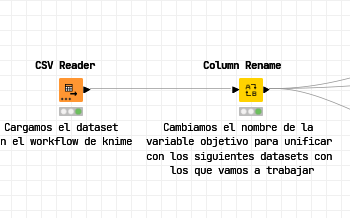
\includegraphics[width = 0.5\textwidth]{dataset02_positive_rename}
    \caption{Cambiamos el nombre de la clase positiva al principio de todo nuestros procesos. Esto lo hacemos para que en los siguientes \emph{datasets} tengamos que hacer los mínimos cambios posibles.}
\end{figure}

Lo primero que merece la pena comentar es que tenemos 20 variables de entrada, y una variable de salida. En nuestro \emph{dataset} tenemos 2000 ejemplos, lo que ya supone un tamaño bastante más grande con respecto al \emph{dataset} anterior.

En el nodo de estadísticas nos fijamos primeramente en la variable de salida. La siguiente figura muestra que tenemos un balanceo perfecto entre las cuatro clases consideradas:

\begin{figure}[H]
    \centering
    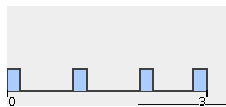
\includegraphics[width = 0.6\textwidth]{dataset02_eda_balanced}
    \caption{Las cuatro clases de salida están perfectamente balanceadas, con 500 ejemplos por cada clase}
\end{figure}

Para el resto de variables, podemos ver las distribuciones de los datos según cada variable, pero no sacamos conclusiones de utilidad. Las distribuciones son bastante normales, como se muestra en la siguiente figura:

\begin{figure}[H]
    \centering
    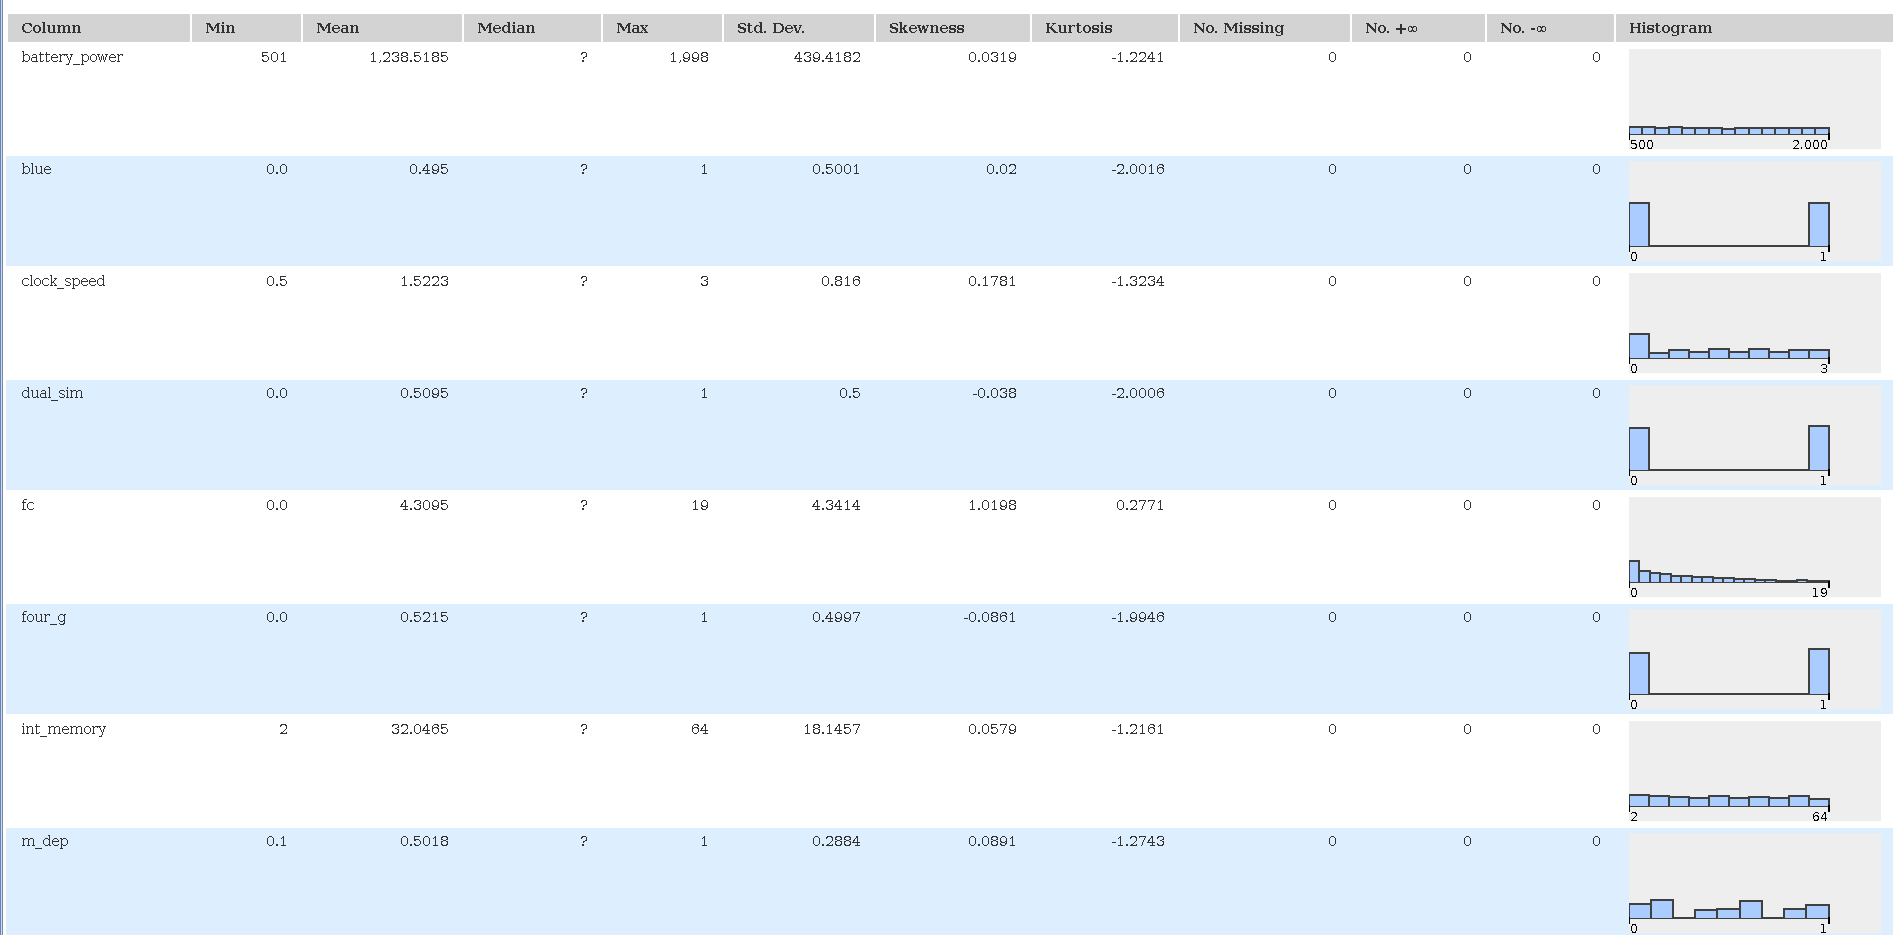
\includegraphics[width = 0.9\textwidth]{dataset02_eda_distribuciones}
    \caption{Las distribuciones según cada variable son bastante normales. Tenemos distribuciones prácticamente uniformes, decrecientes, \ldots No sabemos cómo podríamos explotar esta información.}
\end{figure}

Mostramos ahora la matriz de correlaciones lineales:

\begin{figure}[H]
    \centering
    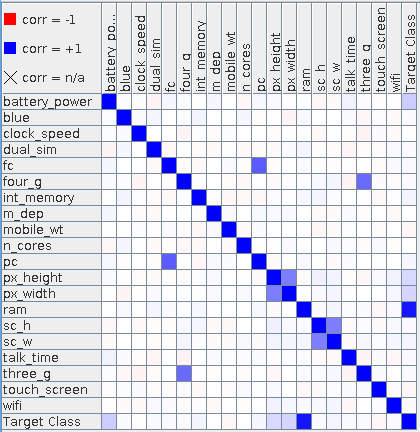
\includegraphics[width = 0.6\textwidth]{dataset02_eda_correlaciones}
    \caption{Matriz de correlaciones lineales. Un color azul significa correlación lineal positiva, y un color rojo significa correlación lineal negativa}
    \label{dataset02_eda_correlaciones:imagen}
\end{figure}

Era de esperar la correlación entre la anchura y altura de píxeles (los móviles suelen guardar unos \emph{aspect ratio} fijados), pero esto no nos es del todo útil, salvo para eliminar una columna, lo que no parece que vaya a tener un impacto enorme. También tenemos la misma correlación con las medidas en la unidad \lstinline{sc_h, sc_w}, y de nuevo nos encontramos en la misma situación.

Lo que sí que es realmente interesante es que la variable que representa la memoria \emph{RAM} correla mucho ($0.917$) con la variable de salida. Por tanto, podemos decir, adelantándonos a lo que comentaremos más adelante, que la memoria \emph{RAM} es un factor decisivo para fijar el precio de un móvil.

Mostramos ahora los \emph{boxplots} de algunas variables:

\begin{figure}[H]
    \centering
    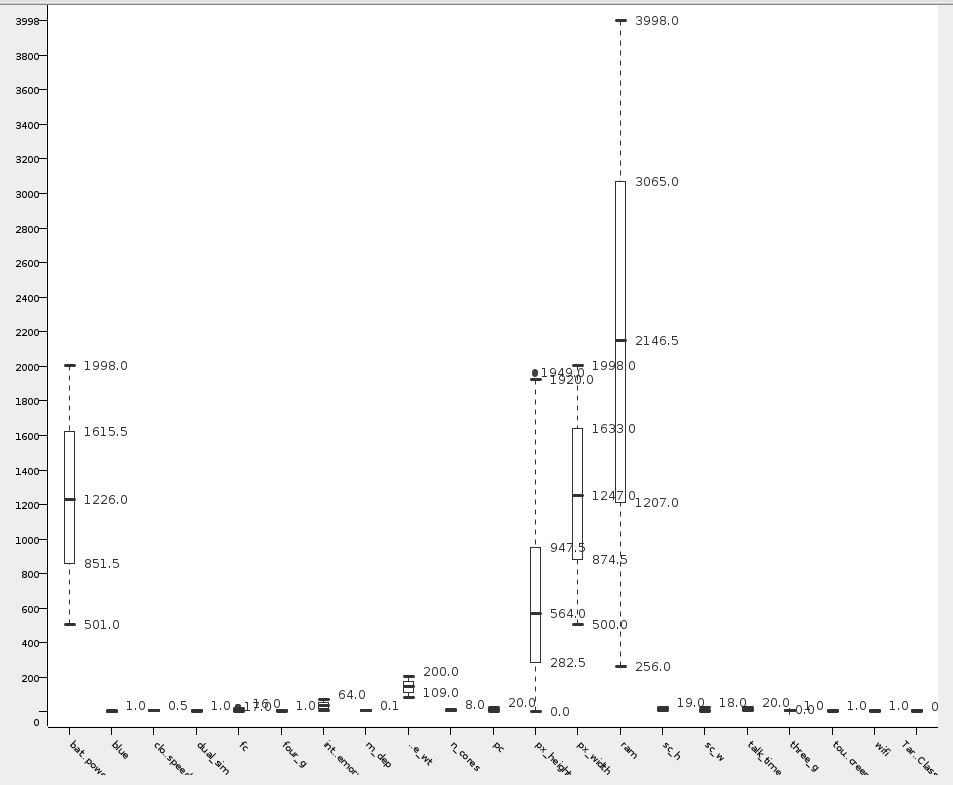
\includegraphics[width = 0.8\textwidth]{dataset02_eda_boxplots}
    \caption{\emph{Boxplots} de algunas variables}
\end{figure}

Queda claro que en este caso también tenemos bastantes \emph{outliers} fijándonos solo en información unidimensional (variable a variable). Por tanto seguiremos borrando \emph{outliers} usando el criterio $3\cdot IQR$.

Mostramos ahora la gráfica de combinar algunas variables dos a dos, sin obtener resultados relevantes, como ya nos ha pasado previamente. Elegimos las variables que mostramos quitando aquellas que mostraban información del todo irrelevante, al menos según nuestra interpretación de esta gráfica:

\begin{figure}[H]
    \centering
    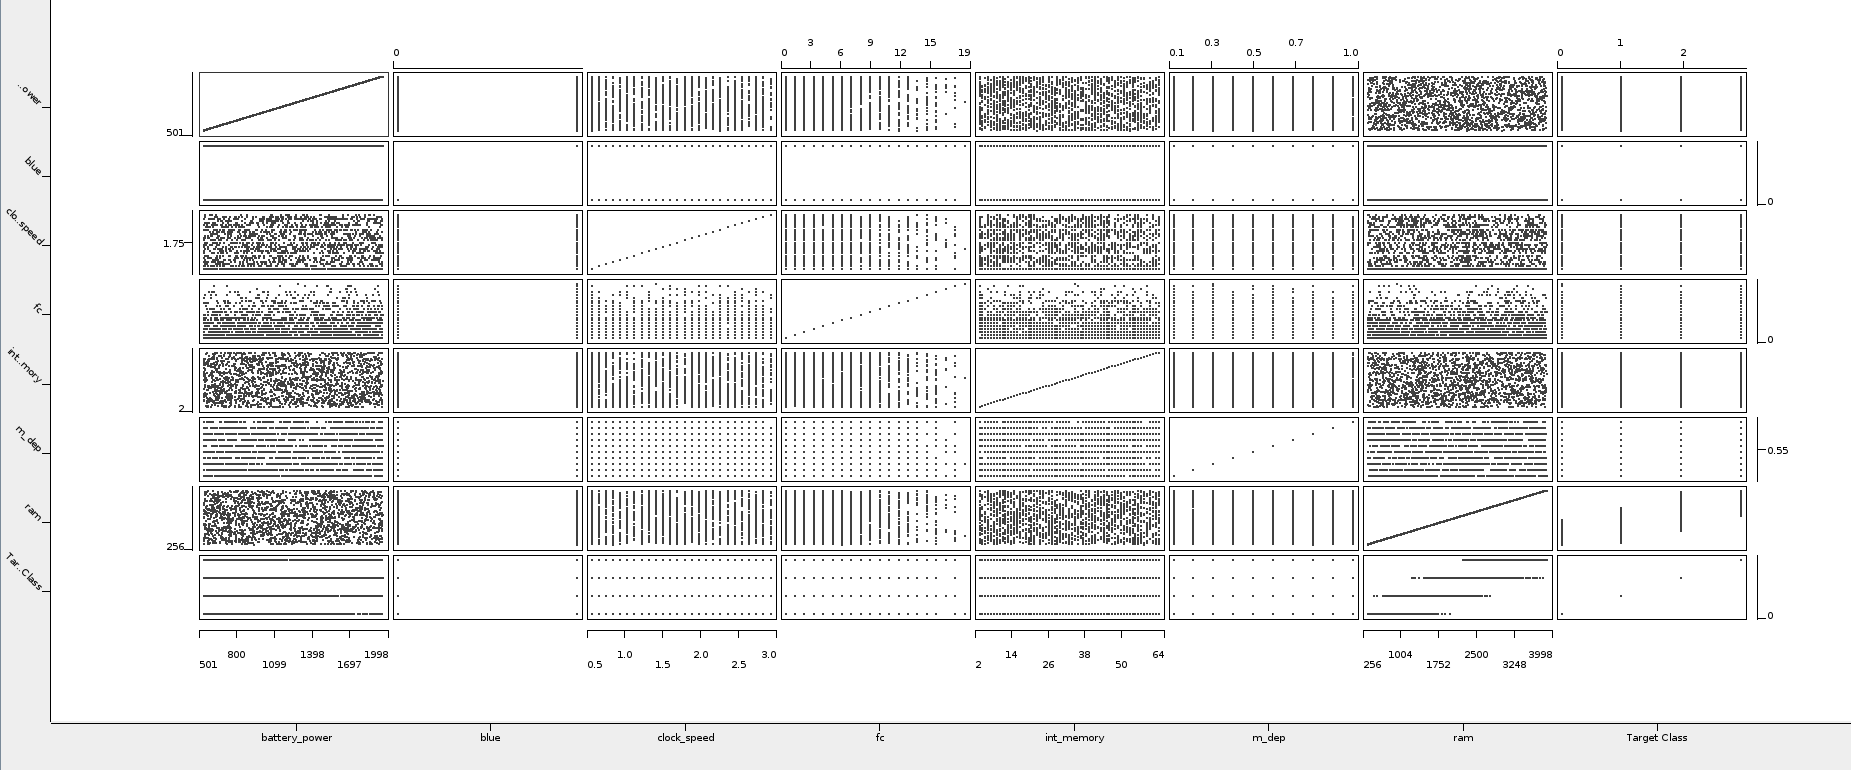
\includegraphics[width = 0.9\textwidth]{dataset02_eda_combinaciones}
    \caption{Gráfica de todas las posibles combinaciones de dos variables de nuestro dataset}
\end{figure}

En último lugar, aplicamos \emph{PCA} para reducir nuestro conjunto de datos a tener dos variables de entrada y la variable de salida. Al igual que hacíamos en el \emph{dataset} anterior, mostramos los resultados visualmente, donde el color indica la clase a la que pertenece cada punto:

\begin{figure}[H]
    \centering
    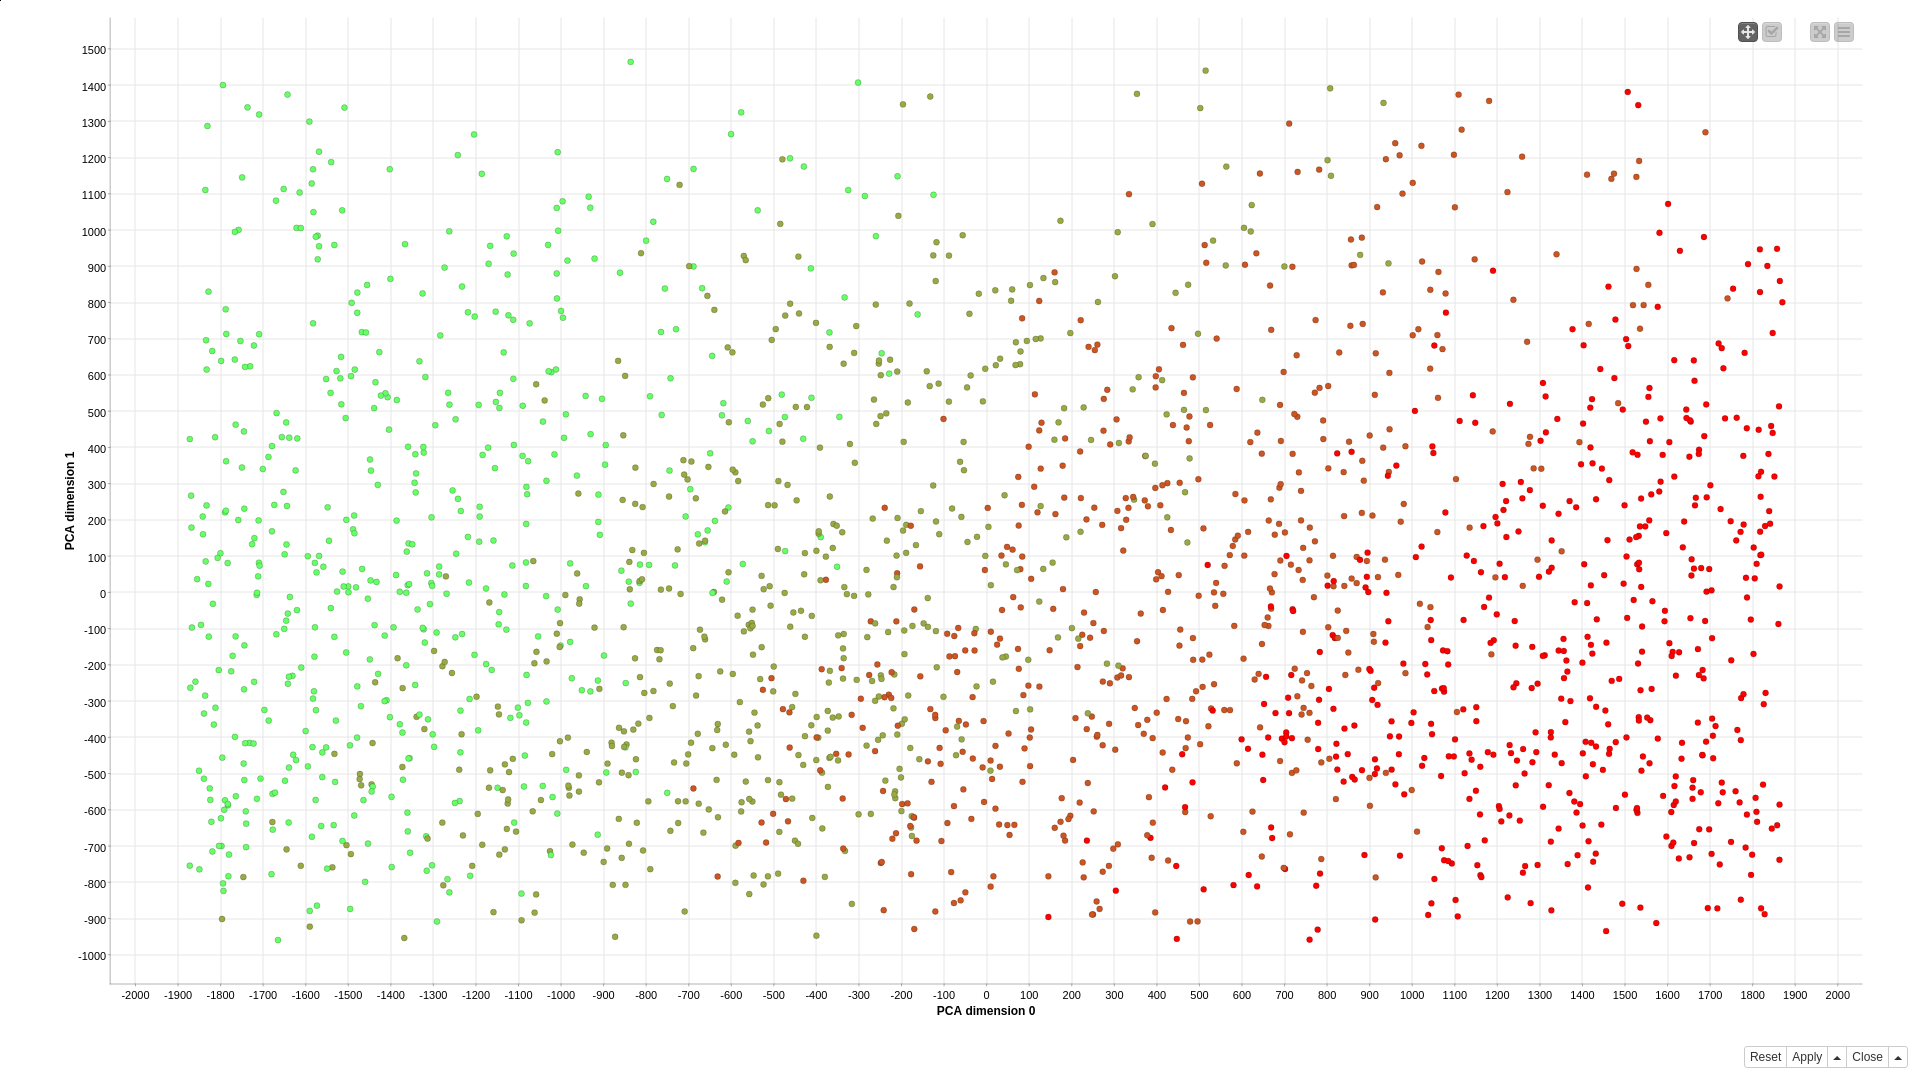
\includegraphics[width = 0.8\textwidth]{dataset02_eda_pca}
    \caption{Resultado de aplicar \emph{PCA} en dos dimensiones, coloreando cada punto según la clase
a la que pertenecen}
\end{figure}

Para este \emph{dataset} obtenemos un resultado muy interesante tras aplicar \emph{PCA}. Gracias al coloreado vemos que los puntos tras transformarse se distribuyen de forma más o menos continua, en un gradiente que va en diagonal decreciente. Esto nos hace pensar que esta transformación, que pasa de 20 variables de entrada a únicamente 2, es útil para considerarse como paso previo a la generación de nuestros modelos de aprendizaje automático.

En último lugar, vemos que no tenemos \emph{missing values} en el \emph{dataset}. El nodo que borra las filas que contienen algún \emph{missing value} deja el \emph{dataset} con las mismas filas, y por tanto no detecta ningún \emph{missing value}.

\pagebreak

\subsection{\emph{Bank Marketing}}

De nuevo, empezamos mostrando la fuente original de \emph{dataset}, que se puede encontrar en \cite{bank_marketing_source:online}. En este caso estamos trabajando con un \emph{dataset} del conocido repositorio \emph{UCI}, y no con \emph{Kaggle} como hemos hecho con los \emph{datasets} previos. En la fuente del \emph{dataset} \cite{bank_marketing_source:online} se dice que el objetivo es: \emph{``The classification goal is to predict if the client will subscribe (yes/no) a term deposit (variable y)''}.

\subsubsection{Análisis Exploratorio de los Datos}

Como ya hemos comentado, el objetivo es predecir si un cliente se suscribirá (salida \emph{yes}) o no (salida \emph{no}). Estamos por tanto ante un problema de clasificación binaria.

Lo primero que vemos es que tenemos 21 columnas (20 variables de entrada y una de salida) y 41188 ejemplos. Por tanto, estamos ante un problema con unas dimensionalidades mucho mayores que las que hemos trabajado hasta ahora.

Comenzamos mostrando la distribución de la variable de salida:

\begin{figure}[H]
    \centering
    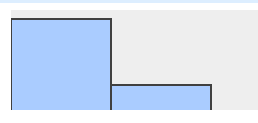
\includegraphics[width = 0.9 \textwidth]{dataset03_eda_balanceo}
    \caption{Distribución de la variable de salida}
\end{figure}

Visualmente, queda claro que tenemos un desbalanceo enorme. La salidas \emph{no} tiene 36548 ejemplos. La salida \emph{yes}, por tanto, tiene 4640 ejemplos. Tenemos por tanto solo un $11.27\%$ de ejemplos para la clase positiva (\emph{yes}).

Como ya hemos repetido anteriormente, las distribuciones de otras variables no nos dan pistas relevantes sobre cómo podemos atacar el problema que se nos presenta:

\begin{figure}[H]
    \centering
    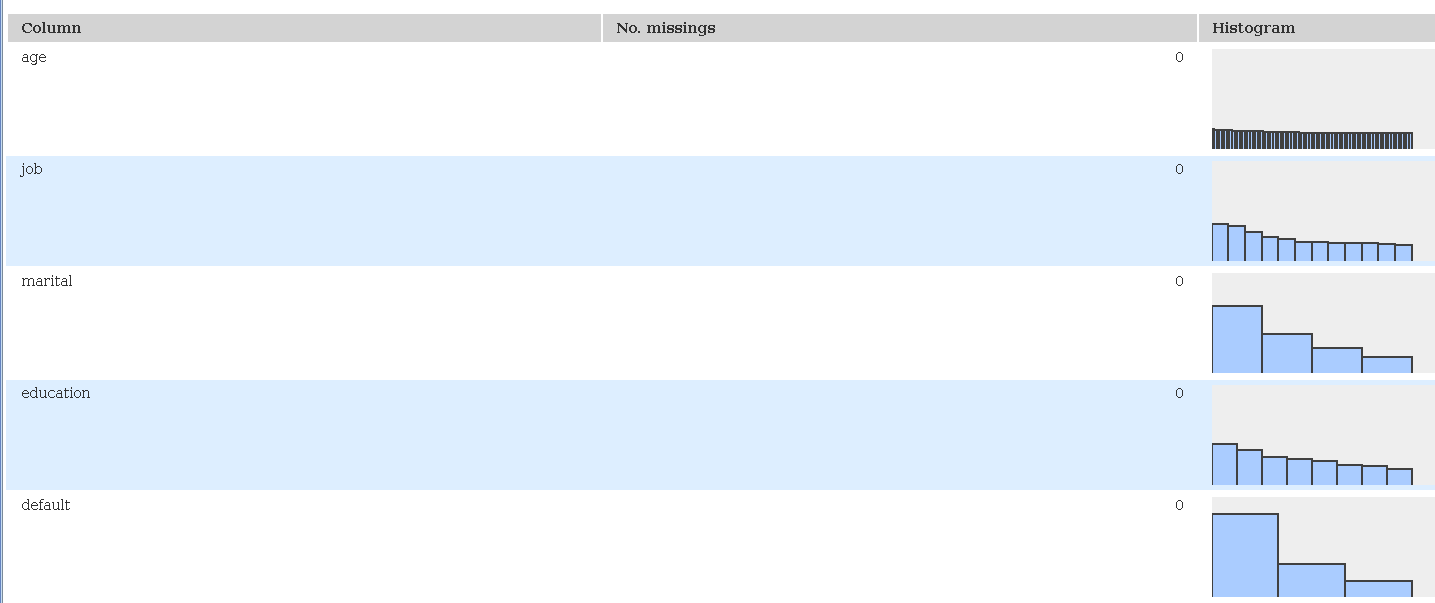
\includegraphics[width = 0.9 \textwidth]{dataset03_eda_distribuciones}
    \caption{Distribuciones de algunas variables de entrada. No sabemos cómo explotar esta información en el problema que estamos estudiando.}
\end{figure}

Consideramos ahora la matriz de correlaciones, que hasta ahora ha sido uno de los puntos clave en este análisis exploratorio de datos:

\begin{figure}[H]
    \centering
    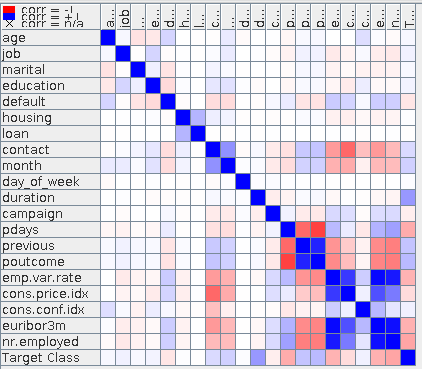
\includegraphics[width = 0.9 \textwidth]{dataset03_eda_correlaciones}
    \caption{Matriz de correlaciones lineales. Un color azul significa correlación lineal positiva, y un color rojo significa correlación lineal negativa}
\end{figure}

Para comenzar, ninguna variable está excesivamente correlada con la variable de salida, así que no nos podemos aprovechar de esto como hemos hecho anteriormente. Sí que tenemos conjuntos de variables que están correladas entre sí, pro ejemplo \lstinline{Emp.var.rate} y \lstinline{cons.price.idx}, o \lstinline{housing} y \lstinline{loan}. Sin embargo, en este \emph{dataset} concreto que presenta otro tipo de problema (el desbalanceo que ya hemos visto), vamos a emplear otras técnicas de procesado de datos.

Mostramos ahora los \emph{boxplots} de algunas variables:

\begin{figure}[H]
    \centering
    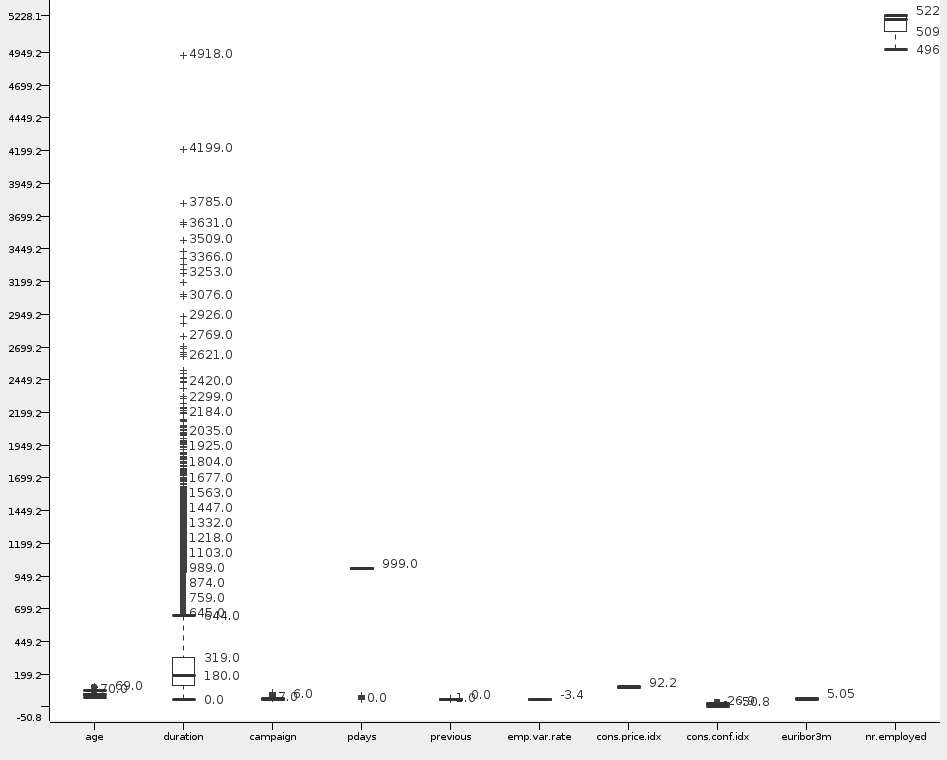
\includegraphics[width = 0.9 \textwidth]{dataset03_eda_boxplot}
    \caption{\emph{Boxplots} de algunas de las variables del \emph{dataset}}
\end{figure}

Claramente hay variables con demasiados \emph{outliers}, por ejemplo \lstinline{duration}. Por tanto, seguimos usando el criterio $3 \cdot IQR$ que llevamos usando toda la práctica para intentar paliar el efecto de estos valores atípicos.

El \emph{plot} de las parejas de variables ha sido tan inútil durante toda la práctica que esta vez no lo mostramos. Se puede consultar en \lstinline{KNIME} expandiendo el nodo correspondiente, pero no hemos sido capaces de extraer información relevante de esta gráfica conjunta.

En último lugar, mostramos el resultado de aplicar \emph{PCA} para obtener solo dos variables de entrada. El resultado, coloreado según la clase de salida, se muestra en la siguiente figura:

\begin{figure}[H]
    \centering
    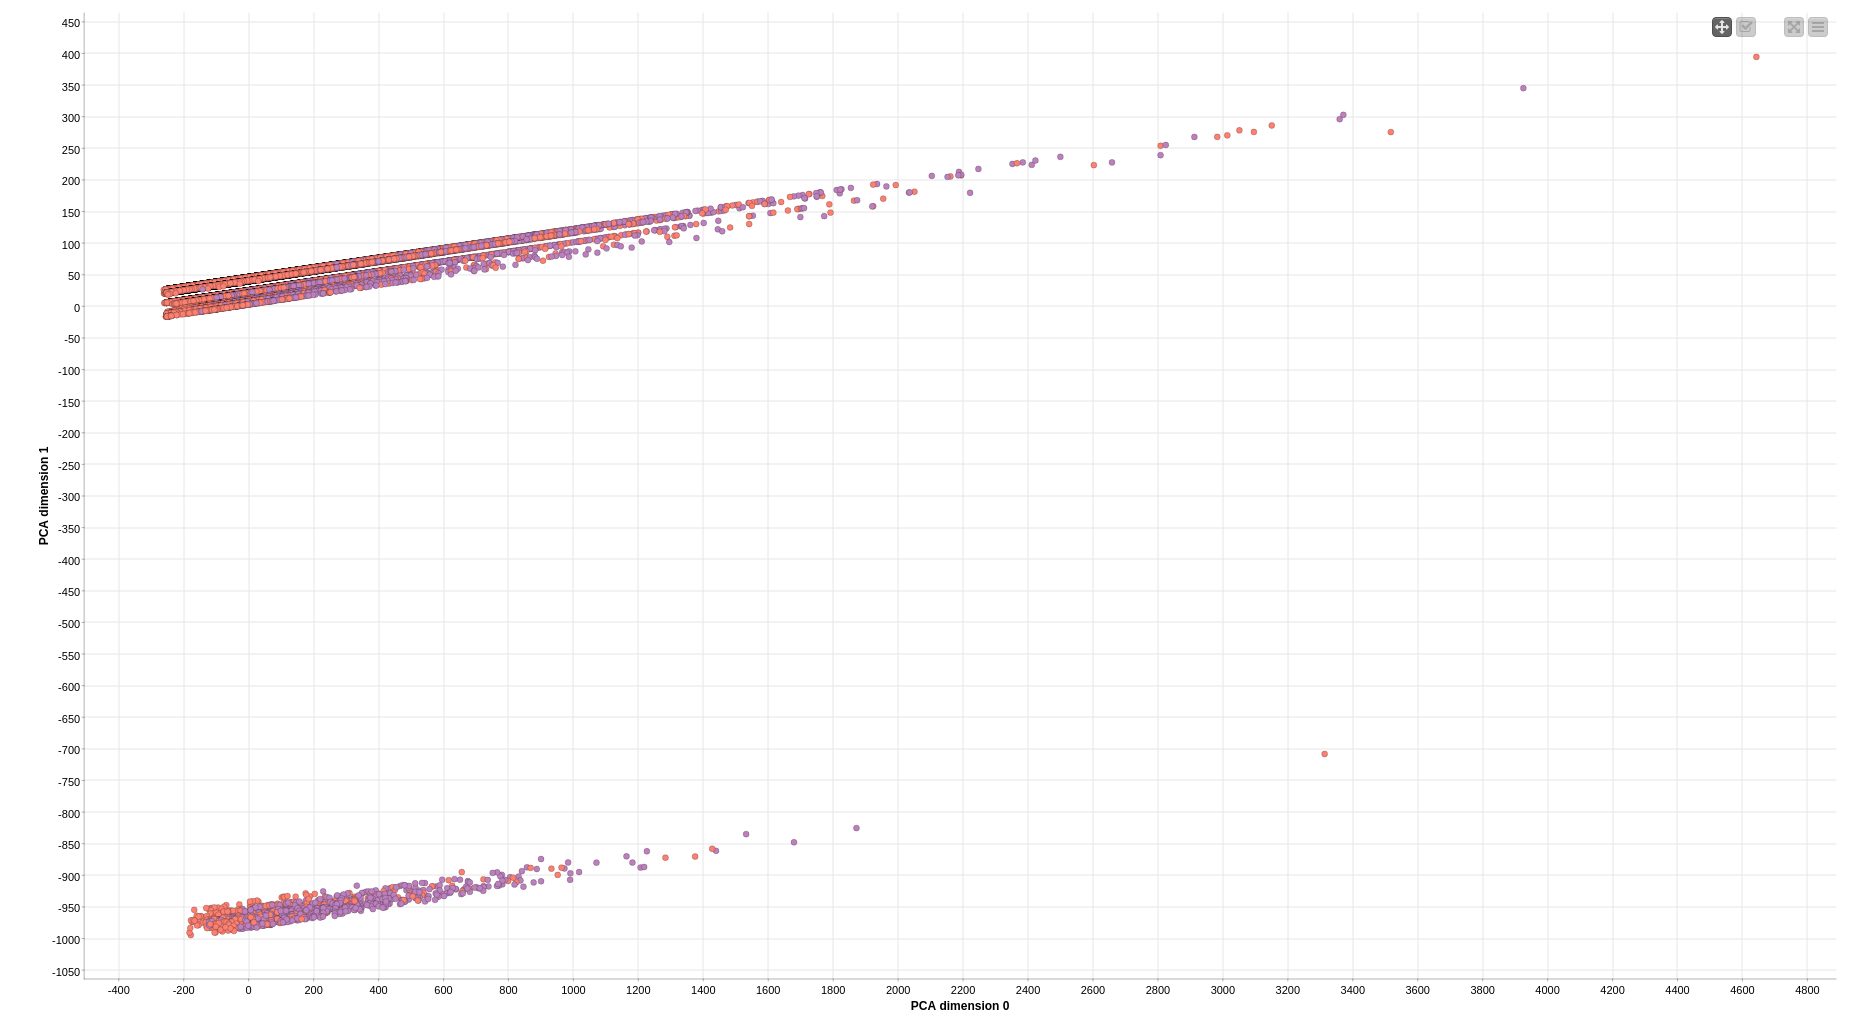
\includegraphics[width = 0.9 \textwidth]{dataset03_eda_pca}
    \caption{Resultado de aplicar \emph{PCA} en dos dimensiones, coloreando cada punto según la clase a la que pertenece}
\end{figure}

Con esta transformación hemos creado dos \emph{clusters} afilados claramente separados. Sin embargo, las dos clases de salida están mezcladas en estos dos \emph{clusters}, y por tanto parece que en este problema \emph{PCA} no va a ser una técnica útil.

Como hemos hecho previamente, borramos aquellas filas que contengan \emph{missing values}. Como el nodo de \lstinline{KNIME} no borra ninguna fila, podemos afirmar que al menos \lstinline{KNIME} no ha detectado ningún \emph{missing value}.

Es destacable comentar que, según lo que indica \cite{bank_marketing_source:online}, hay variables que tienen valores especiales. Por ejemplo, un valor de $999$ en \lstinline{pdays} indica que el cliente no ha sido previamente contactado. Si tuviésemos el tiempo y herramientas necesarias, esto habría que tratarlo de una mejor forma. Por ejemplo, añadiendo una variable adicional que sea un \emph{flag} de este hecho. Sin embargo esto tampoco es óptimo. Por tanto, hay que tener esto en cuenta en el rendimiento de nuestros modelos.

\pagebreak

\subsection{Tanzania Water Pump}

Para este \emph{dataset}, la fuente original de los datos no es ni \emph{Kaggle} ni \emph{UCI}, sino \emph{DrivenData}, otro famoso repositorio de \emph{datasets}. Los datos originales (los nuestros pueden haber sido ligeramente modificados por los profesores) se encuentran en \cite{tanzania_source:online}.

En la fuente original de los datos \cite{tanzania_source:online}, se dice que el problema a resolver en este \emph{dataset} es: \emph{``Using data from Taarifa and the Tanzanian Ministry of Water, can you predict which pumps are functional, which need some repairs, and which don't work at all?''}. Por tanto, tenemos que conseguir clasificar las fuentes como funcionales o no funcionales. Por ser más relevantes, consideramos como la clase positiva aquella que indica que una fuente \textbf{no} es funcional.

\subsubsection{Análisis Exploratorio de Datos}

Partimos de un \emph{dataset} que tiene x filas y 23123 columnas. Por tanto, estamos trabajando con un \emph{dataset} realmente grande, tanto en altura como anchura. Para tratar de hacer el problema más manejable, elegimos las columnas con las que vamos a trabajar usando la matriz de correlaciones lineales. Dicha matriz de correlaciones se muestra a continuación:

\begin{figure}[H]
    \centering
    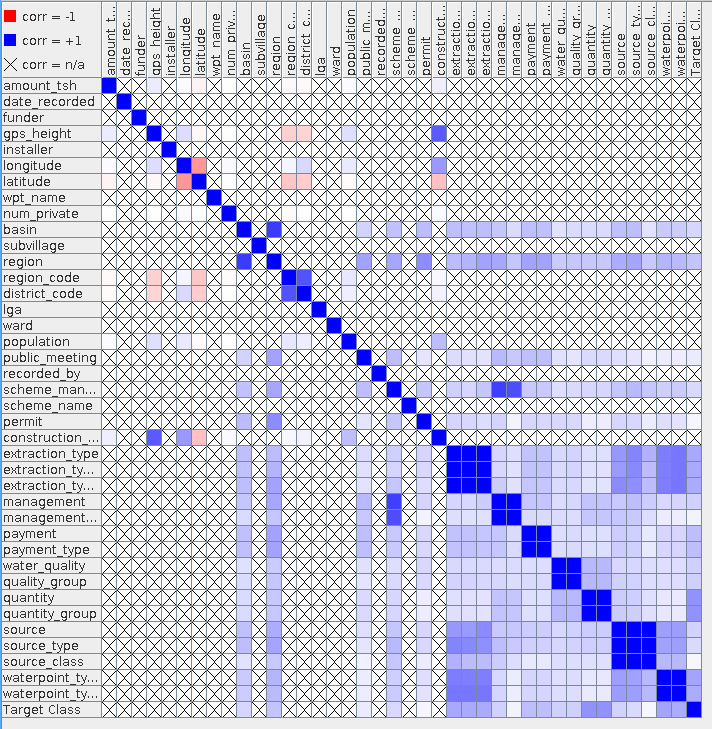
\includegraphics[width = 0.9 \textwidth]{dataset04_eda_correlaciones}
    \caption{Matriz de correlaciones lineales. Un color azul significa correlación lineal positiva, y un color rojo significa correlación lineal negativa}
\end{figure}

El proceso de filtrado se muestra en el siguiente \emph{workflow}:

\begin{figure}[H]
    \centering
    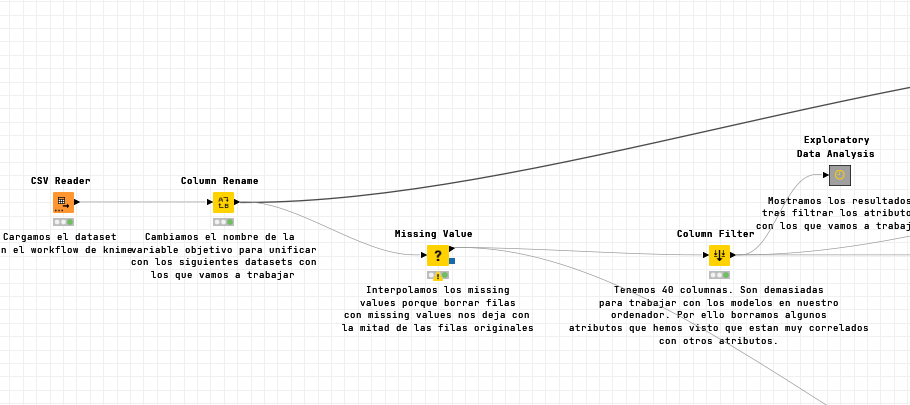
\includegraphics[width = 0.9 \textwidth]{dataset04_filtrado_columnas}
    \caption{Consideramos un árbol de clasificación, y usando la relevancia de las variables, seleccionamos las columnas que vamos a usar}
\end{figure}

Tras esto realizo el siguiente filtrado:

\begin{itemize}
    \item Quito \lstinline{extraction_type:_group, class} y me quedo con \lstinline{extraction_type}
    \item Quito \lstinline{source_:type, class} y me quedo con \lstinline{source}
    \item Quito \lstinline{waterpoint_type} y me quedo con \lstinline{waterpoint}
    \item Quito \lstinline{management_group, scheme_managemente} y me quedo con \lstinline{management}
    \item Quito \lstinline{basin} y me quedo con \lstinline{region}
    \item Quito \lstinline{district_code} y me quedo con \lstinline{region_code}
    \item Quito \lstinline{payment_type} y me quedo con \lstinline{payment}
    \item Quito \lstinline{quality_group} y me quedo con \lstinline{water_quality}
    \item Quito \lstinline{quantity_group} y me quedo con \lstinline{quantity}
\end{itemize}

Tras este filtrado, pasamos de tener 40 columnas a tener 28, con lo cual estamos haciendo que el problema sea más manejable. A partir de aquí el \emph{EDA} se realiza sobre el conjunto de datos filtrado. Mostramos de nuevo la matriz de correlaciones:

\begin{figure}[H]
    \centering
    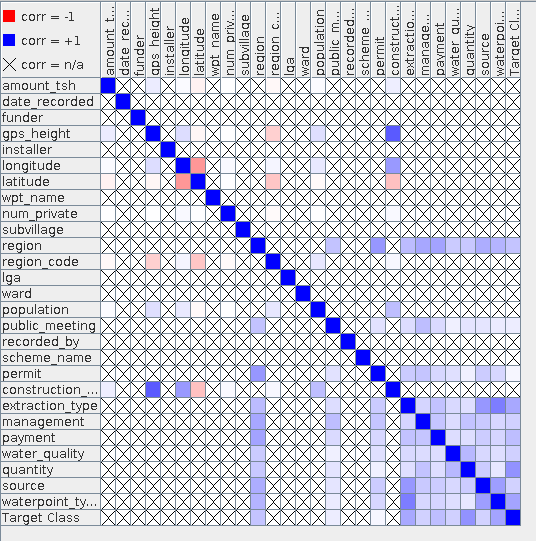
\includegraphics[width = 0.7 \textwidth]{dataset04_eda_correlaciones_filtrado}
    \caption{Matriz de correlaciones lineales tras realizar el filtrado de las variables. Un color azul significa correlación lineal positiva, y un color rojo significa correlación lineal negativa}
\end{figure}

Con esto queda claro que hemos generado un conjunto de datos más sencillo al tener menos variables de entrada. Además es un \emph{dataset} más ortogonal, es decir, con menos correlaciones entre las variables de entrada.

Mostramos ahora la distribución de la variable de salida:

\begin{figure}[H]
    \centering
    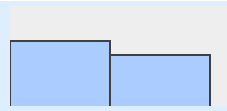
\includegraphics[width = 0.4 \textwidth]{dataset04_eda_desbalanceo}
    \caption{Distribución de la variable de salida}
\end{figure}

La clase de salida está ligeramente desbalanceada. En otros \emph{dataset} no nos habría preocupado, pero al tener un \emph{dataset} con tantos ejemplos, un ligero desbalanceo relativo puede suponer muchos ejemplos de diferencia. Por tanto, en este caso también aplicaremos \emph{SMOTE} para realizar el balanceo de las clases.

En todos los \emph{datasets} anteriores mostrar la distribución de algunas variables ha sido inútil. Este \emph{dataset} no es la excepción, así que no mostramos dichas distribuciones pues no hemos sido capaces de explotar esa información.

Mostramos los \emph{boxplots} de algunas variables:

\begin{figure}[H]
    \centering
    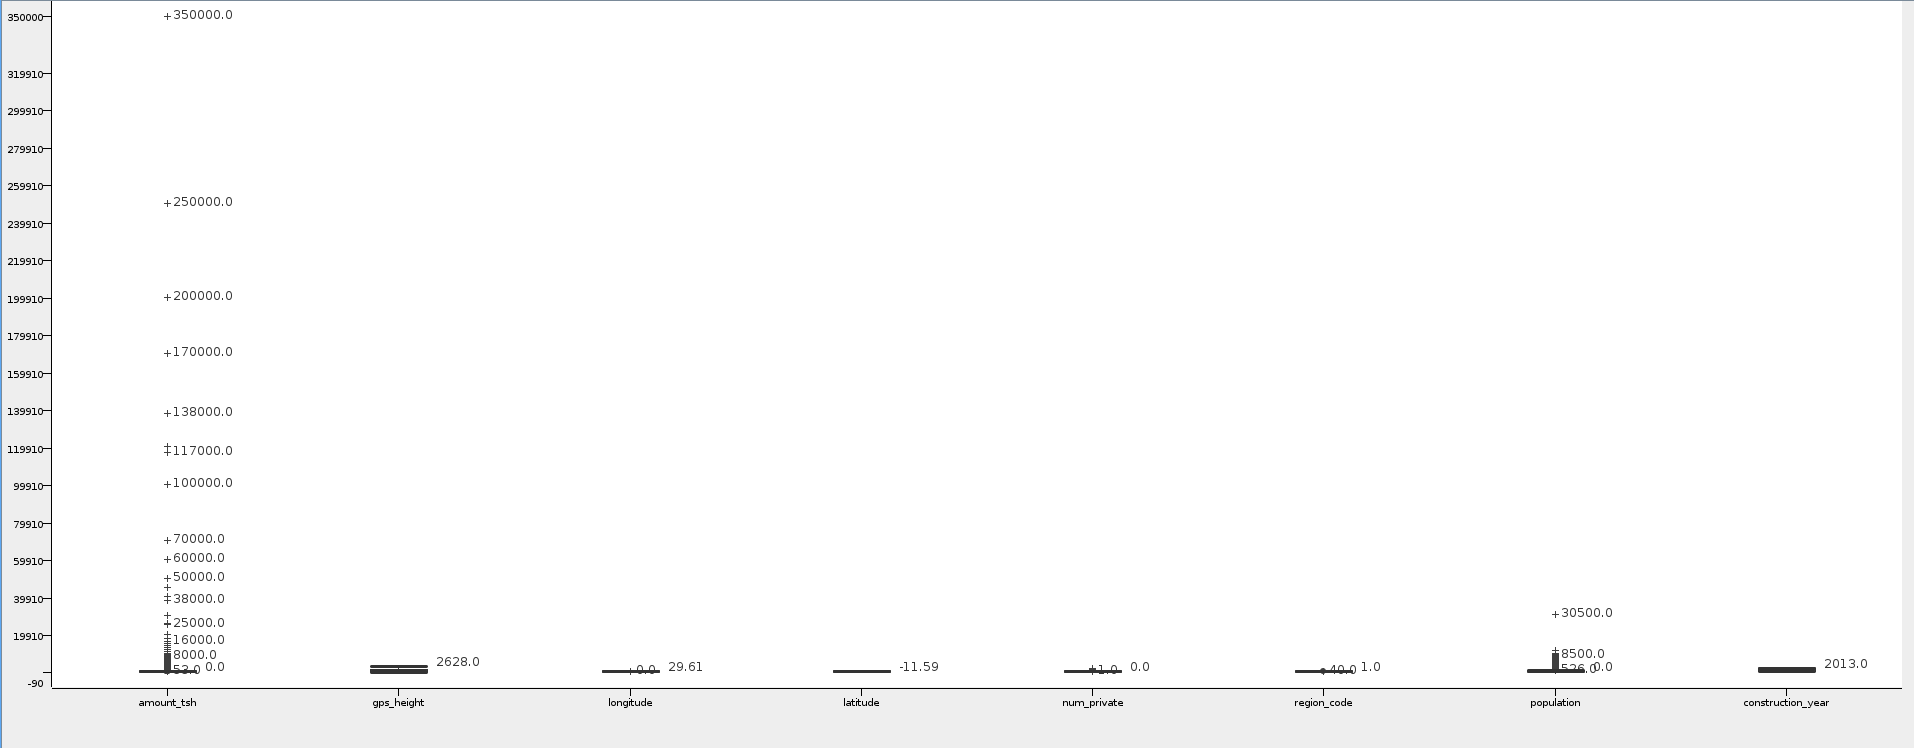
\includegraphics[width = 0.8 \textwidth]{dataset04_eda_boxplot}
    \caption{\emph{Boxplots} de algunas de las variables con las que trabajamos}
\end{figure}

Como viene siendo habitual, tenemos algunos \emph{outliers}, que de nuevo tratamos con el criterio $3 \cdot IQR$.

Mostramos ahora el resultado de aplicar \emph{PCA} buscando reducir la dimensionalidad del problema a solo dos variables de entrada:

\begin{figure}[H]
    \centering
    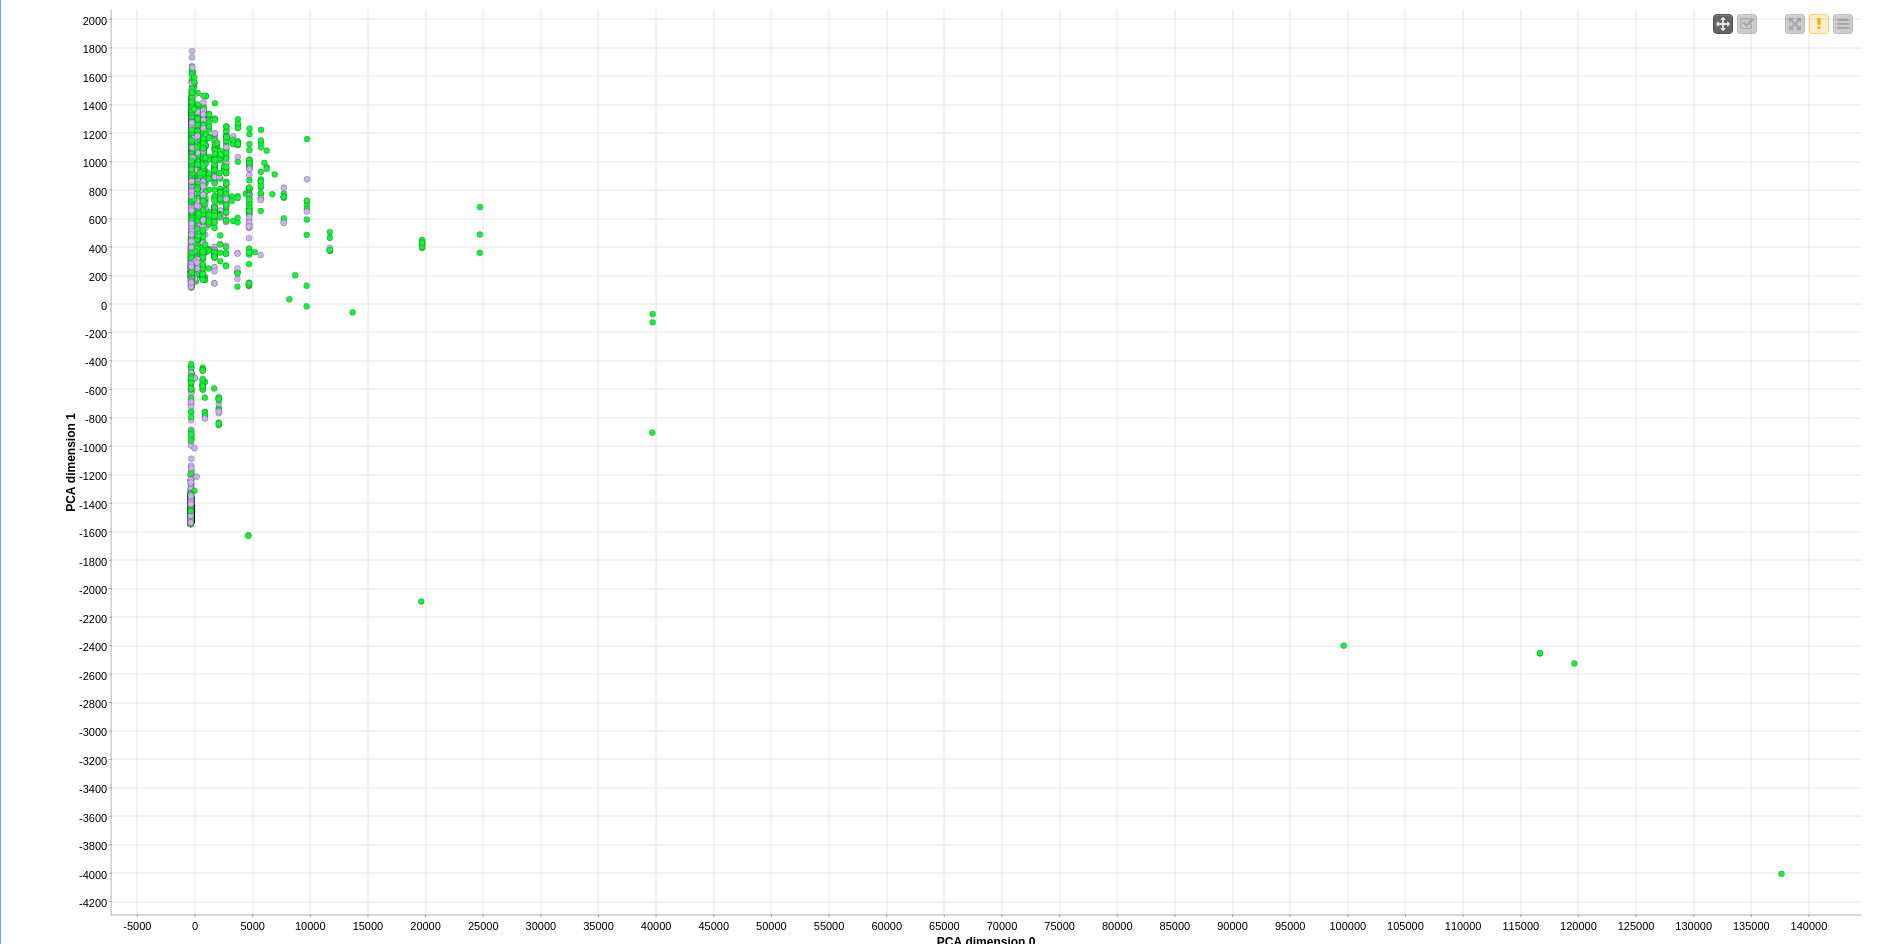
\includegraphics[width = 0.8 \textwidth]{dataset04_eda_pca}
    \caption{Resultado de aplicar \emph{PCA} en dos dimensiones, coloreando cada punto según la clase a la que pertenece}
\end{figure}

No encontramos ningún patrón interesante que explotar. Cabe también mencionar que, \lstinline{KNIME} con toda la potencia de nuestro equipo, no es capaz de mostrar todos los puntos que componen el \emph{dataset}. Pero aún así hemos probado experimentalmente a entrenar modelos previa aplicación \emph{PCA}, sin resultados satisfactorios.

Para acabar, usamos nuestro nodo que borra las filas con \emph{missing values}. Esto provocaba que borrásemos aproximadamente la mitad de los datos, una pérdida que no nos podemos permitir. Por ello, aplicamos interpolación lineal para los valores numéricos y el valor más frecuente para los valores categóricos.

Sabemos que lo ideal habría sido interpolar estos valores usando predictores entrenados sobre la parte del \emph{dataset} que no tiene \emph{missing values}. Sin embargo, por falta de tiempo, no exploramos este camino y usamos la interpolación simple que ya hemos comentado..

\pagebreak

\section{Resultados Obtenidos} \label{resultados_brutos:seccion}

\subsection{Consideraciones iniciales} \label{cv_consideraciones:seccion}

Para esta práctica, hemos considerado 7 modelos de aprendizaje automático distintos, que puedan ser interesantes para los cuatro problemas a los que nos vamos a enfrentar. Algunos de estos modelos pueden tener muy poco sentido para algún problema concreto. Sin embargo, elegimos los mismo 7 modelos para los 4 datasets, porque esto nos permitirá realizar una comparación entre ellos en distintos ambientes. De hecho, el que algunos modelos no tengan sentido en ciertas situaciones será una buena conclusión a extraer en el análisis posterior.

Los modelos considerados son:

\begin{enumerate}
    \item Árbol de decisión construido con \emph{AdaBoost}
    \item Red Neuronal Simple
    \item \emph{Support Vector Machine}
    \item \emph{Support Vector Machine} con normalización
    \item \emph{K-NN}
    \item \emph{Naive Bayes}
    \item \emph{Random Forest}
\end{enumerate}

Pensamos que con estos modelos tenemos una variedad suficiente para comparar en situaciones diferentes. Además, todos los los modelos tienen sentido para al menos uno de los \emph{datasets} con los que vamos a trabajar.

En este proceso, usaremos un nodo al que llamamos \emph{Custom Cross Validation}. Este nodo tiene la misma base que el nodo de \lstinline{KNIME} \emph{Cross Validation}. Sin embargo, añadimos dos nodos, uno para preprocesar el \emph{fold} de entrenamiento y otro para aplicar dicho preprocesado al \emph{test}, sin hacer \emph{data snooping}. Es decir, las operaciones se calculan y aplican con \emph{training}, y se aplican en \emph{test} \textbf{usando el cálculo realizado sobre \emph{training}}.

En \customcite{heart_failure_cross_validation:seccion} mostraremos de forma extensa los distintos \emph{workflows} que componen nuestras siete validaciones cruzadas. Sin embargo, para los siguientes \emph{datasets} no repetiremos el mismo proceso, para evitar ser demasiado repetitivos y extensos. Solo mostraremos aquellas partes en las que haya diferencias con lo mostrado en \customcite{heart_failure_cross_validation:seccion} y con los \emph{datasets} desarrollados previamente.

\pagebreak

\subsection{Heart Failure Prediction} \label{heart_failure_cross_validation:seccion}

\subsubsection{\emph{Workflows} empleados para \emph{Cross Validation}} \label{dataset01_capturas_cv:seccion}

En primer lugar, tenemos un \emph{metanodo} para encapsular todo el trabajo con los 7 algoritmos que hemos considerado. Este \emph{metanodo} se mostraba en el \emph{workflow} más general en \customcite{workflow_general:imagen}. Dentro de este nodo para \emph{Cross Validation} tenemos la siguiente estructura:

\begin{figure}[H]
    \centering
    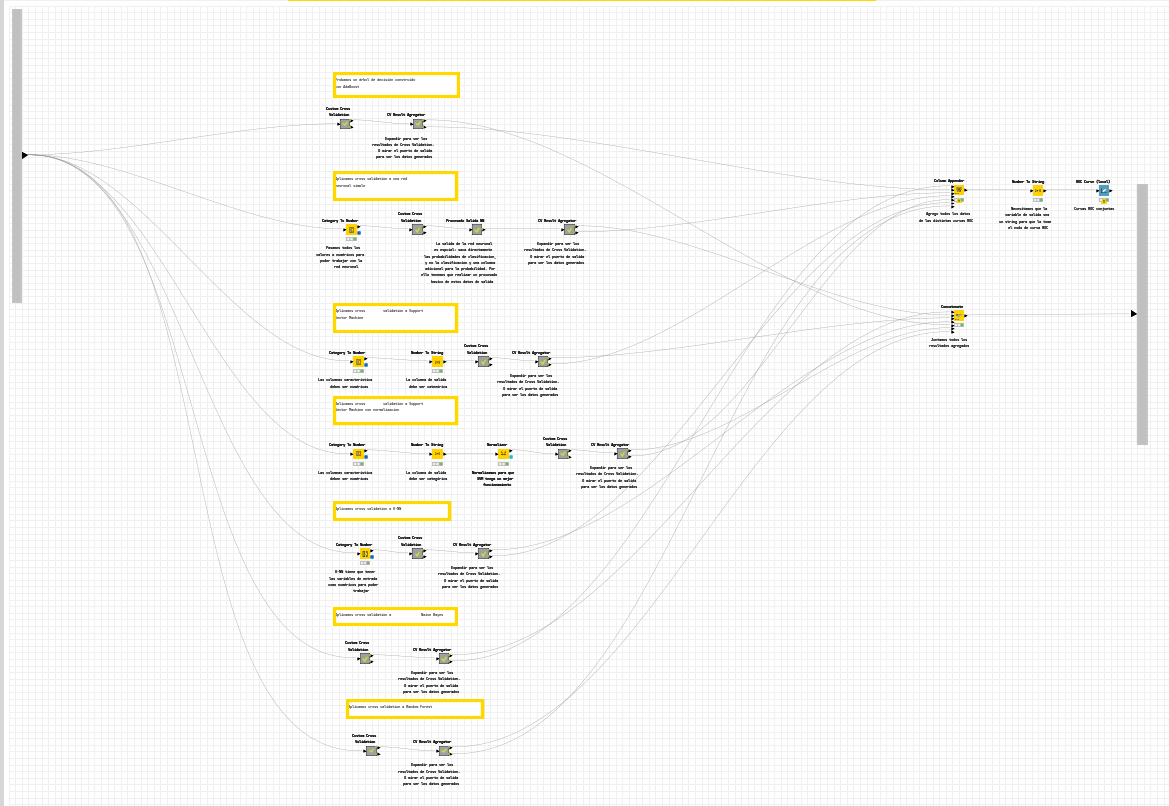
\includegraphics[width = 0.9 \textwidth]{dataset01_cross_validation_workflow}
    \caption{\emph{Workflow} en el que realizamos todos los \emph{Cross Validation} de los algoritmos considerados}
\end{figure}

Mostramos una captura con mayor \emph{zoom} para que se vea claramente la estructura generada, dejando sin mostrar alguna de las filas correspondientes a algunos de los 7 modelos estudiados:

\begin{figure}[H]
    \centering
    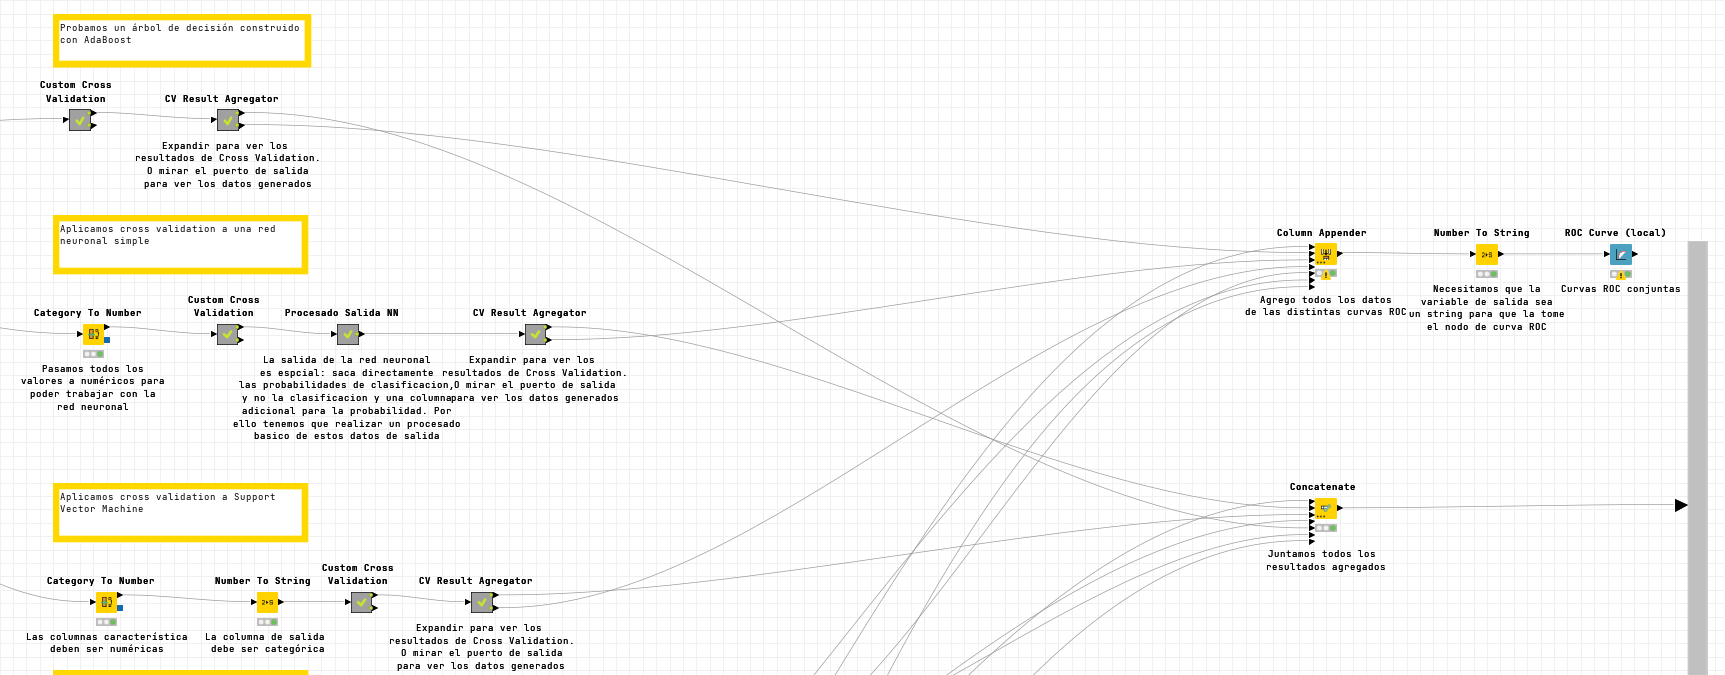
\includegraphics[width = 0.9 \textwidth]{dataset01_cross_validation_workflow_zoom}
    \caption{\emph{Workflow} en el que realizamos todos los \emph{Cross Validation} de los algoritmos considerados, con algo de \emph{zoom} para que se aprecie mejor la estructura desarrollada}
    \label{cross_val_zoom:image}
\end{figure}

Mostramos el contenido del nodo \emph{Custom Cross Validation} para \emph{AdaBoost}. Este nodo \emph{Custom Cross Validation} tiene ciertas diferencias como ya hemos mencionado en \customcite{cv_consideraciones:seccion}:

\begin{figure}[H]
    \centering
    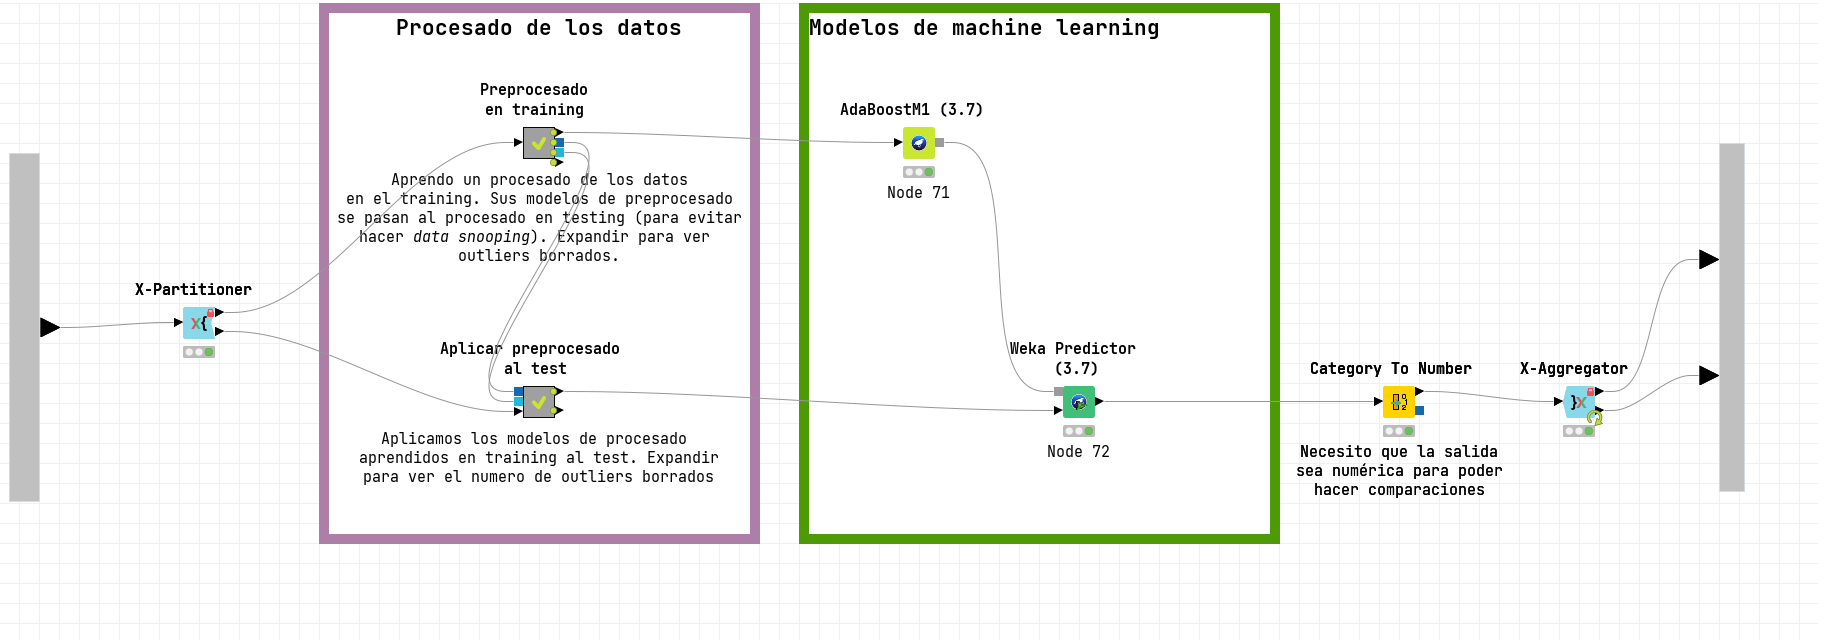
\includegraphics[width = 0.9 \textwidth]{dataset01_cv_adaboost}
    \caption{Nodo de \emph{Cross Validation} para \emph{AdaBoost}}
\end{figure}

Mostramos ahora el nodo para preprocesamiento en \emph{training}:

\begin{figure}[H]
    \centering
    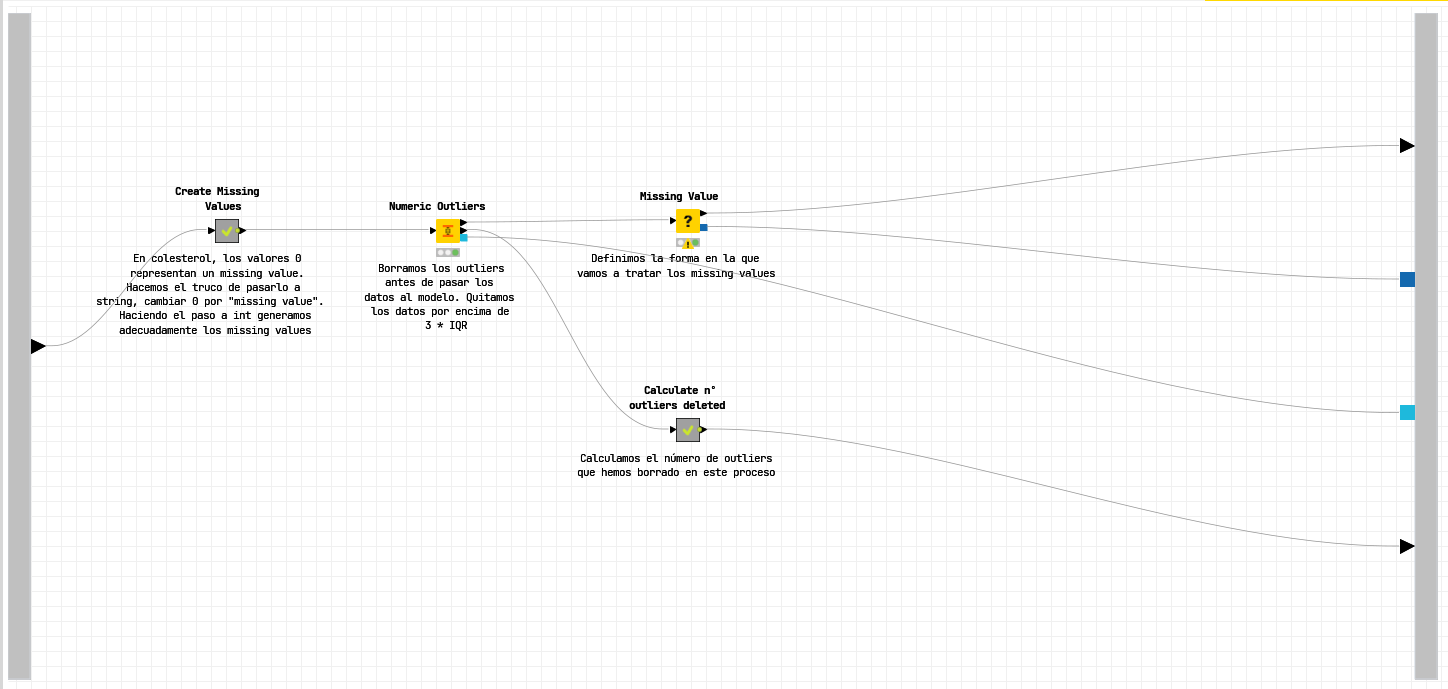
\includegraphics[width = 0.9 \textwidth]{dataset01_cv_pretraining}
    \caption{Preprocesamiento de los datos del \emph{fold} de \emph{training}}
\end{figure}

En esta figura se muestran dos partes fundamentales del procesamiento en este \emph{dataset}. La primera es que, como ya comentábamos, tenemos \emph{missing values} en la columna \lstinline{Cholesterol} marcados con el valor 0. \lstinline{KNIME} no detecta esto como \emph{missing values}, así que empleamos el nodo \emph{Create Missing Values} para marcarlos como tal.

En segundo lugar, tratamos los \emph{outliers} para intentar reducir algo el ruido. Para ello, borramos aquellos valores que distan de la media más de tres veces la desviación típica (fundamentándonos en las propiedades de una distribución normal, en la que la mayoría de los datos están en el intervalo $[\mu - \sigma, \mu + \sigma]$ \cite{intervalos_normal:online}).

Mostramos el nodo \emph{Create Missing Values} para dejar claro el proceso que hemos descrito previamente:

\begin{figure}[H]
    \centering
    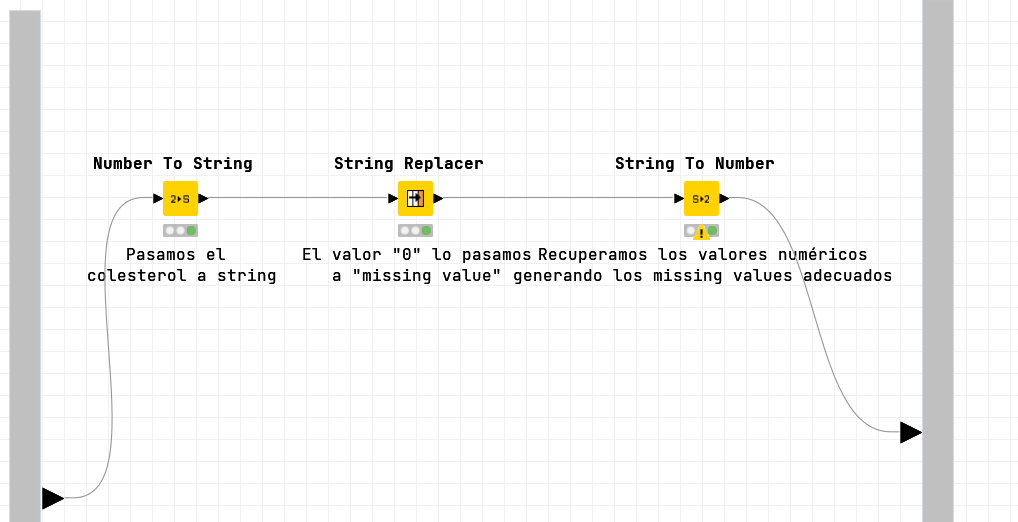
\includegraphics[width = 0.9 \textwidth]{dataset01_cv_createmissingvalues}
    \caption{Nodo que usamos para crear los \emph{Missing Values} que \lstinline{KNIME} no detecta}
    \label{pretest:imagen}
\end{figure}

Mostramos ahora el nodo para preprocesamiento en \emph{test}:

\begin{figure}[H]
    \centering
    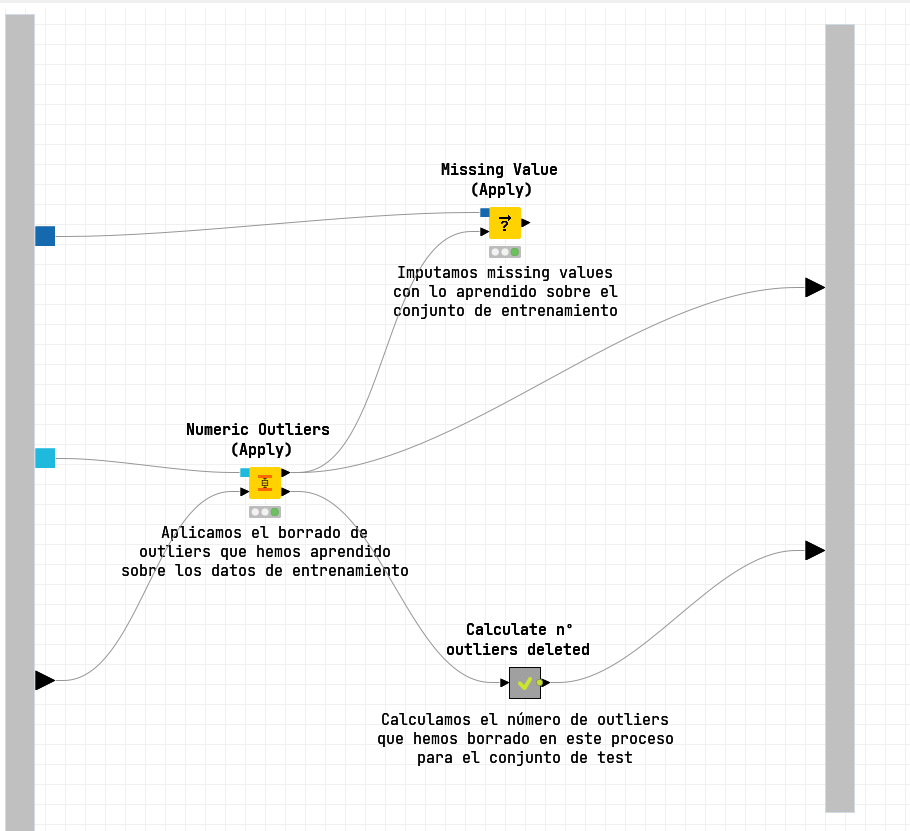
\includegraphics[width = 0.9 \textwidth]{dataset01_cv_pretest}
    \caption{Preprocesamiento de los datos del \emph{fold} de \emph{test}}
    \label{pretest:imagen}
\end{figure}

En \customcite{pretest:imagen} queda claro lo que ya comentábamos, preprocesamos usando los parámetros de procesamiento calculados sobre el \emph{fold} de \emph{training}. Esto es fundamental para \textbf{evitar hacer \emph{data snooping}}.

Además, de ahora en adelante, salvo que se diga lo contrario, estos dos nodos de preprocesamiento serán exactamente los mismos en todos los nodos de \emph{Custom Cross Validation}, en todos los \emph{dataset}, salvo que se indique lo contrario.

Como se muestra en \customcite{cross_val_zoom:image}, estamos pasando la salida de \emph{Custom Cross Validation} a un nodo de procesamiento, que mostramos a continuación:

\begin{figure}[H]
    \centering
    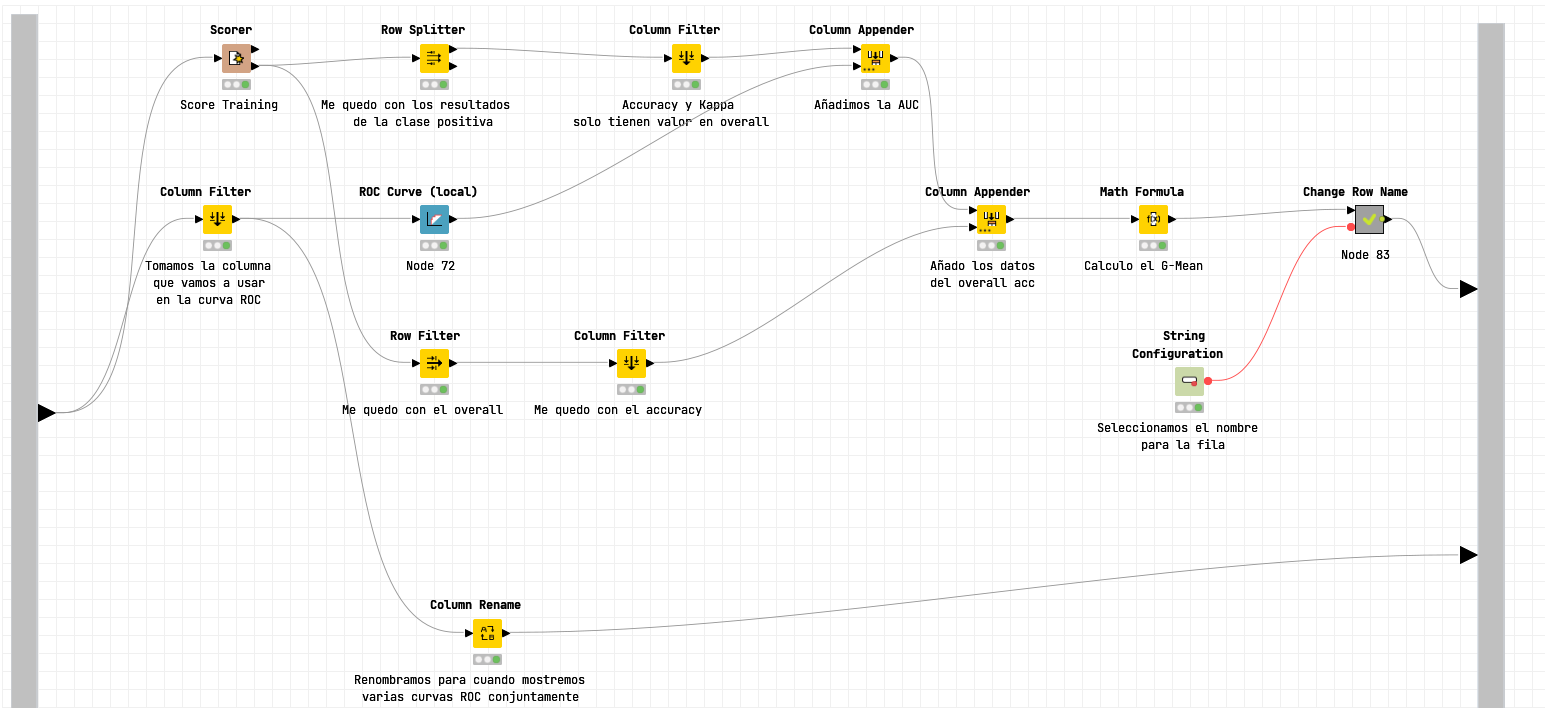
\includegraphics[width = 0.9 \textwidth]{dataset01_cv_process_node}
    \caption{Nodo de procesamiento de la salida de \emph{Custom Cross Validation}}
\end{figure}

En este nodo, tomamos la salida del \emph{scorer} y la procesamos, tomando las métricas para la clase positiva y añadiendo el área debajo de la curva \emph{ROC}. Además, calculamos la fórmula de la métrica \emph{G-Mean}. También devolvemos las probabilidades en bruto para poder calcular las curvas \emph{ROC} globales.

Se muestra también que estamos usando una \lstinline{flow variable} para establecer el nombre del modelo cuyos resultados estamos procesando. Esto es útil para que en las tablas globales, cada fila esté etiquetada por el nombre del modelo que estamos tratando (esto es lo que consigue el nodo \emph{Change Row Name}).

De nuevo, salvo que se diga lo contrario, todos los nodos de este tipo son idénticos.

Mostramos ahora el \emph{workflow} para redes neuronales simples. Realizamos un preprocesado general básico antes de usar nuestro nodo \emph{Custom Cross Validation} que mostramos en la siguiente figura:

\begin{figure}[H]
    \centering
    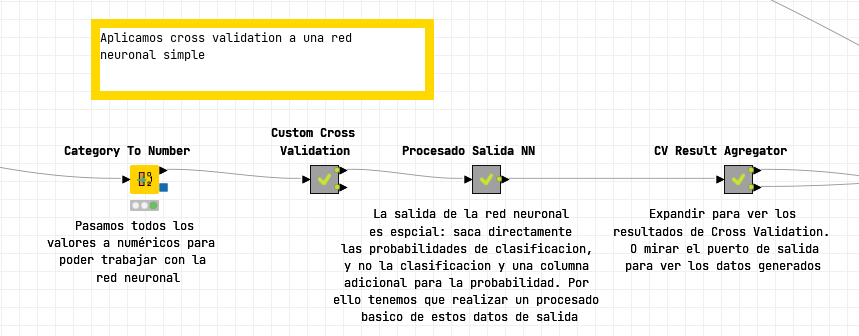
\includegraphics[width = 0.9 \textwidth]{dataset01_cv_pregeneral_nn}
    \caption{Preprocesado general previo a probar Redes Neuronales simples}
\end{figure}

Con esto queda claro que lo único que estamos realizando es pasar todas las variables categóricas a numéricas, pues esto es un requerimiento de las redes neuronales para que puedan funcionar. Mostramos el nodo de \emph{Custom Cross Validation} para este caso:

\begin{figure}[H]
    \centering
    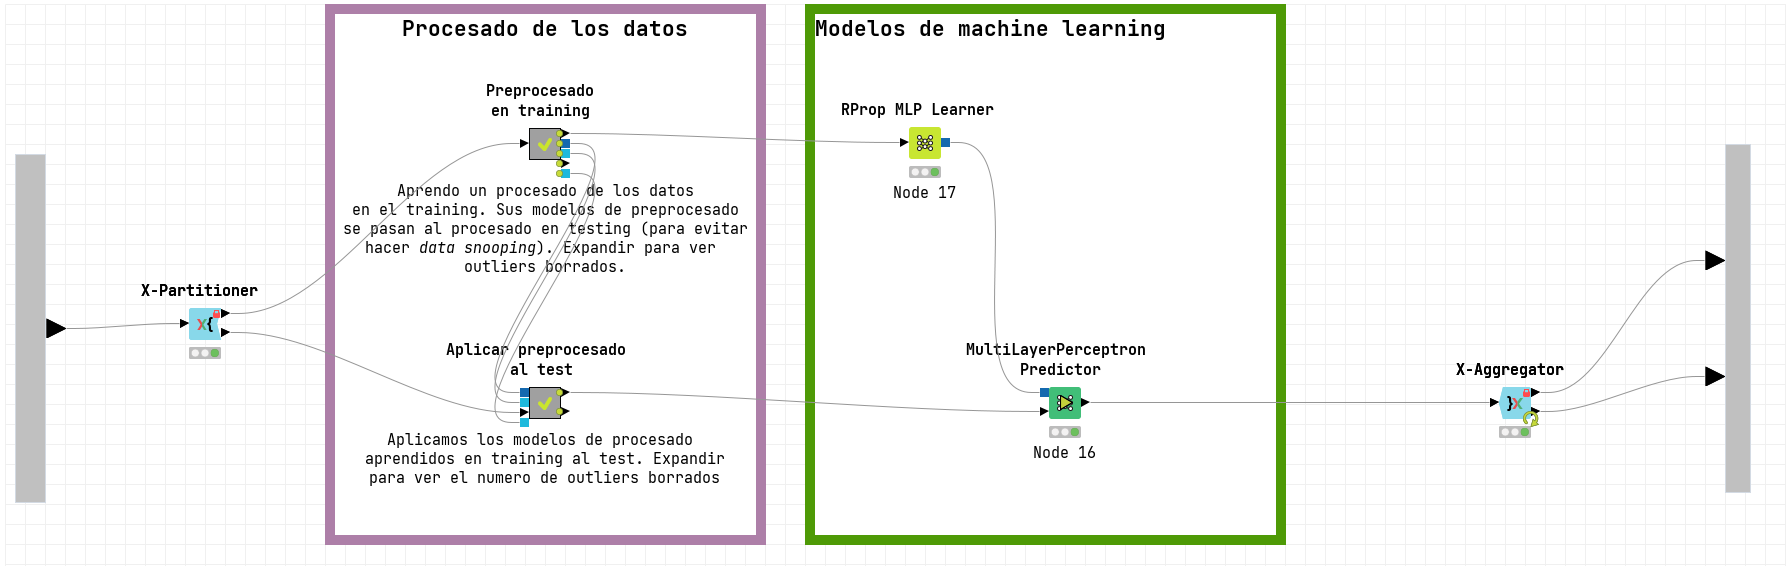
\includegraphics[width = 0.9 \textwidth]{dataset01_cv_nn}
    \caption{Nodo de \emph{Cross Validation} para \emph{Neural Net}}
\end{figure}

En este caso no estamos normalizando las variables, lo cual puede generar resultados no óptimos (pues las redes neuronales se benefician mucho de que las variables de entrada estén normalizadas. De hecho en \emph{deep learning} se usa \emph{batch normalization} para normalizar las salidas entre capas ocultas). Por simpleza del modelo no hacemos esta normalización para el \emph{dataset}, pero en siguientes \emph{datasets} sí que haremos la normalización.

La salida de las redes neuronales suponen un caso concreto que tratar. La red neuronal no nos da la clasificación directamente, sino un valor $x \in [0, 1]$. Tenemos que tratar la salida a mano. Para ello duplicamos la salida de este valor $x$ que representa la probabilidad de clasificación que usaremos para las curvas \emph{ROC}. En una de las dos ramas, colapsamos ese valor al conjunto $\{0, 1 \}$ redondeando, y consideramos eso la salida de clasificación. Mostramos ese proceso, que se hace en el nodo de \emph{Procesado Salida NN}, en la siguiente figura:

\begin{figure}[H]
    \centering
    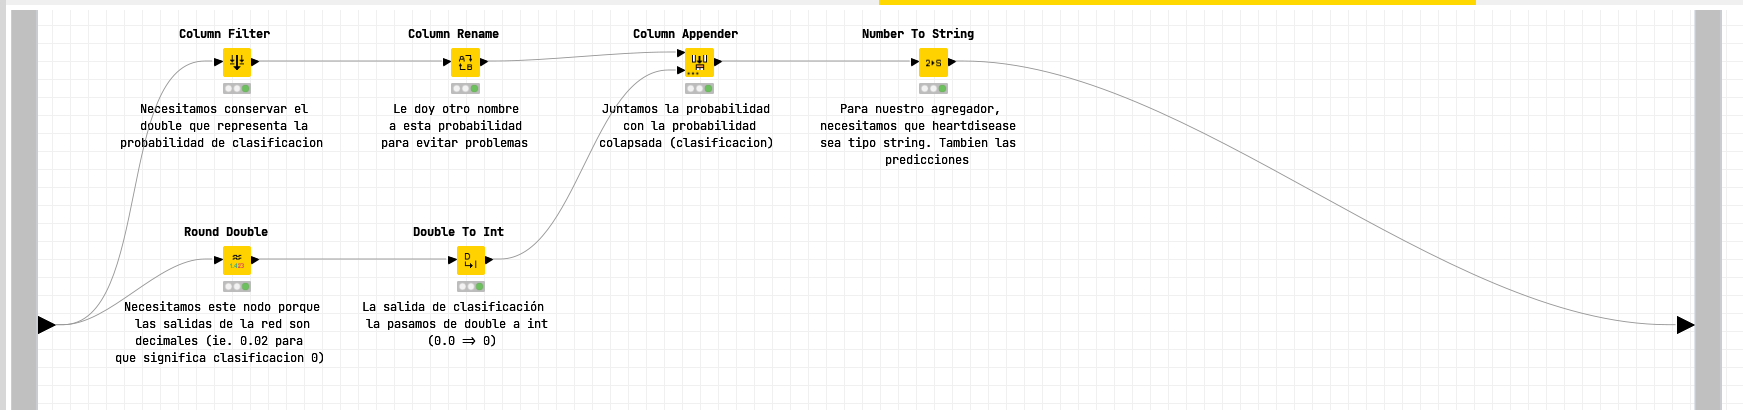
\includegraphics[width = 0.9 \textwidth]{dataset01_cv_procesado_salida}
    \caption{Procesado de la salida de \emph{Neural Net}}
\end{figure}

Con esto, usamos el nodo que procesa la salida de \emph{Cross Validation} que ya hemos mostrado previamente, y que no volvemos a mostrar para evitar ser repetitivos.

Mostramos ahora el preprocesado general para \emph{Support Vector Machine}. Consiste en pasar a variables numéricas todas las variables menos la de salida, que debe ser de tipo categórica:

\begin{figure}[H]
    \centering
    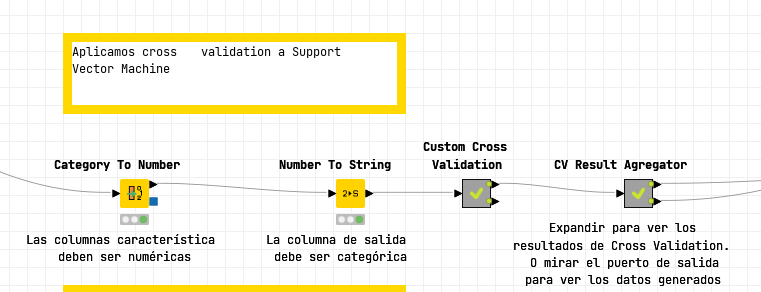
\includegraphics[width = 0.9 \textwidth]{dataset01_cv_pregeneral_svm}
    \caption{Preprocesado general previo a probar \emph{Support Vector Machine}}
\end{figure}

Mostramos ahora el nodo \emph{Custom Cross Validation} para este modelo:

\begin{figure}[H]
    \centering
    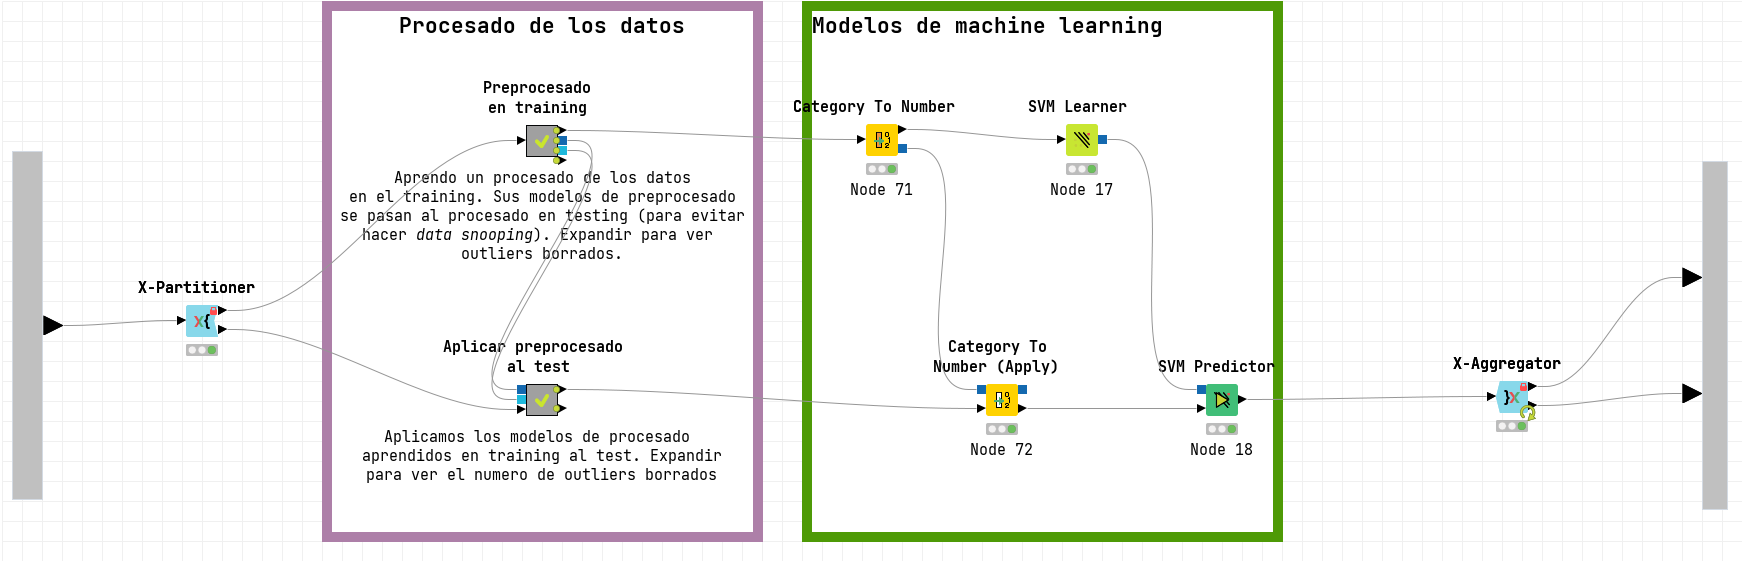
\includegraphics[width = 0.9 \textwidth]{dataset01_cv_svm}
    \caption{Nodo de \emph{Cross Validation} para \emph{Support Vector Machine}}
\end{figure}

En este caso, nos aseguramos de nuevo que estamos usando variables numéricas para las variables de entrada. En este \emph{dataset}, usamos los nodos de \lstinline{KNIME} para \emph{SVM}. En otros \emph{datasets} donde la eficiencia sea clave, pasaremos a usar los nodos de \emph{Weka} que aparentemente funcionan de forma más rápida.

En el caso de \emph{Supoort Vector Machine} con normalización, lo único que cambiamos es el preprocesado general que aplicamos antes de \emph{Custom Cross Validation}. Mostramos esto a continuación:

\begin{figure}[H]
    \centering
    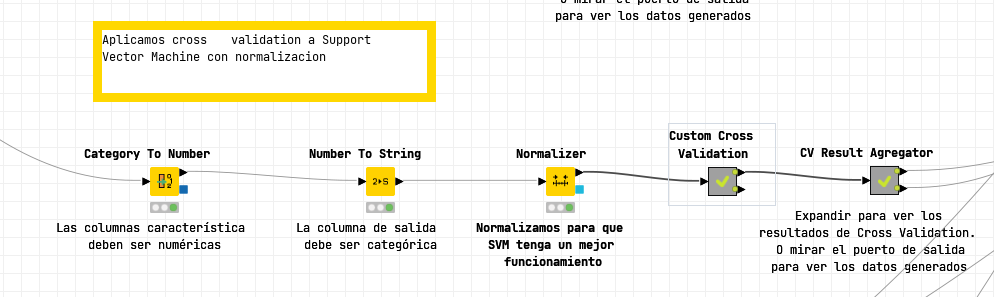
\includegraphics[width = 0.9 \textwidth]{dataset01_cv_pregeneral_svm_norm}
    \caption{Preprocesado general previo a probar \emph{Support Vector Machine} con normalización. Esto es lo único que cambia respecto al modelo anterior: \emph{SVM} sin normalización}
\end{figure}

Mostramos ahora el preprocesado general para \emph{K-NN}. \emph{K-NN} tiene que trabajar con todas las variables de entrada en formato numérico, y esto es lo que hacemos:

\begin{figure}[H]
    \centering
    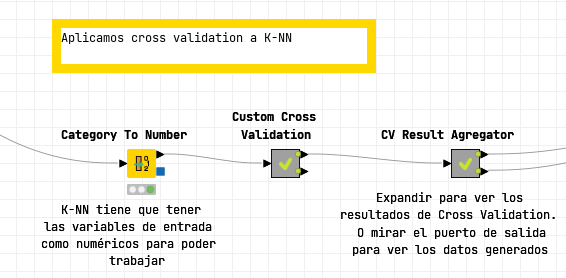
\includegraphics[width = 0.9 \textwidth]{dataset01_cv_pregeneral_knn}
    \caption{Preprocesado general previo a probar \emph{K-NN}}
\end{figure}

Dentro del nodo de \emph{Custom Cross Validation} lo que hacemos es, de nuevo asegurar que tenemos las variables en el formato correcto, y formatear la salida de \emph{K-NN} para que el nodo \emph{X-Aggregator} pueda funcionar correctamente. Mostramos esto a continuación:

\begin{figure}[H]
    \centering
    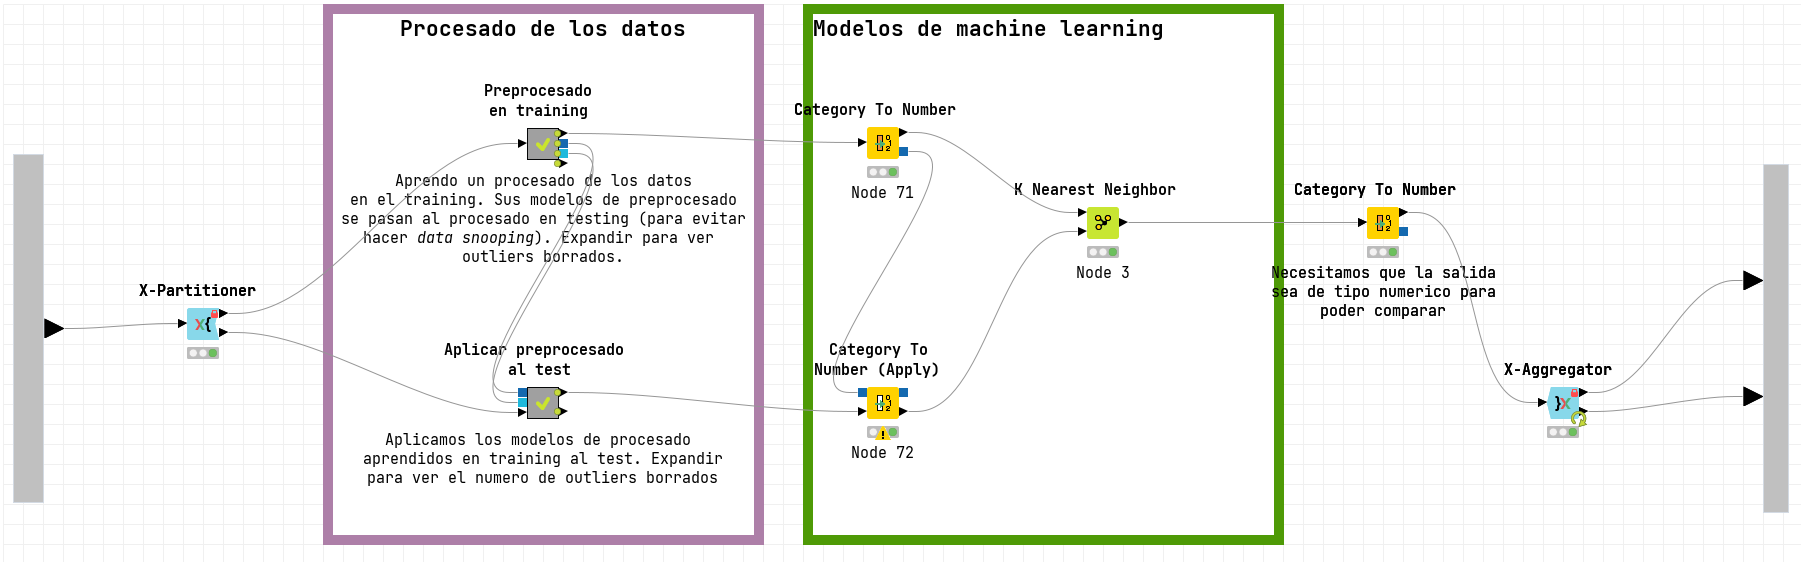
\includegraphics[width = 0.9 \textwidth]{dataset01_cv_knn}
    \caption{Nodo de \emph{Cross Validation} para \emph{K-NN}}
\end{figure}

Mostramos ahora el preprocesado general para \emph{Naive Bayes}. En este caso, no estamos realizando ningún preprocesado general:

\begin{figure}[H]
    \centering
    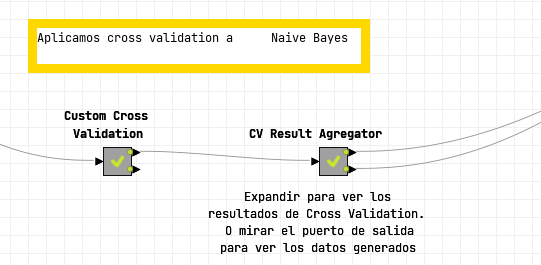
\includegraphics[width = 0.9 \textwidth]{dataset01_cv_pregeneral_naivebayes}
    \caption{Preprocesado general previo a probar \emph{Naive Bayes}. En este caso no estamos realizando ningún tipo de preprocesado previo a \emph{Custom Cross Validation}}
\end{figure}

Mostramos lo que hacemos dentro del nodo \emph{Custom Cross Validation}. No realizamos ningún preprocesado adicional además de los que ya hemos comentado previamente. La salida la pasamos a valores numéricos, para que el nodo \lstinline{X-Aggregator} pueda trabajar correctamente:

\begin{figure}[H]
    \centering
    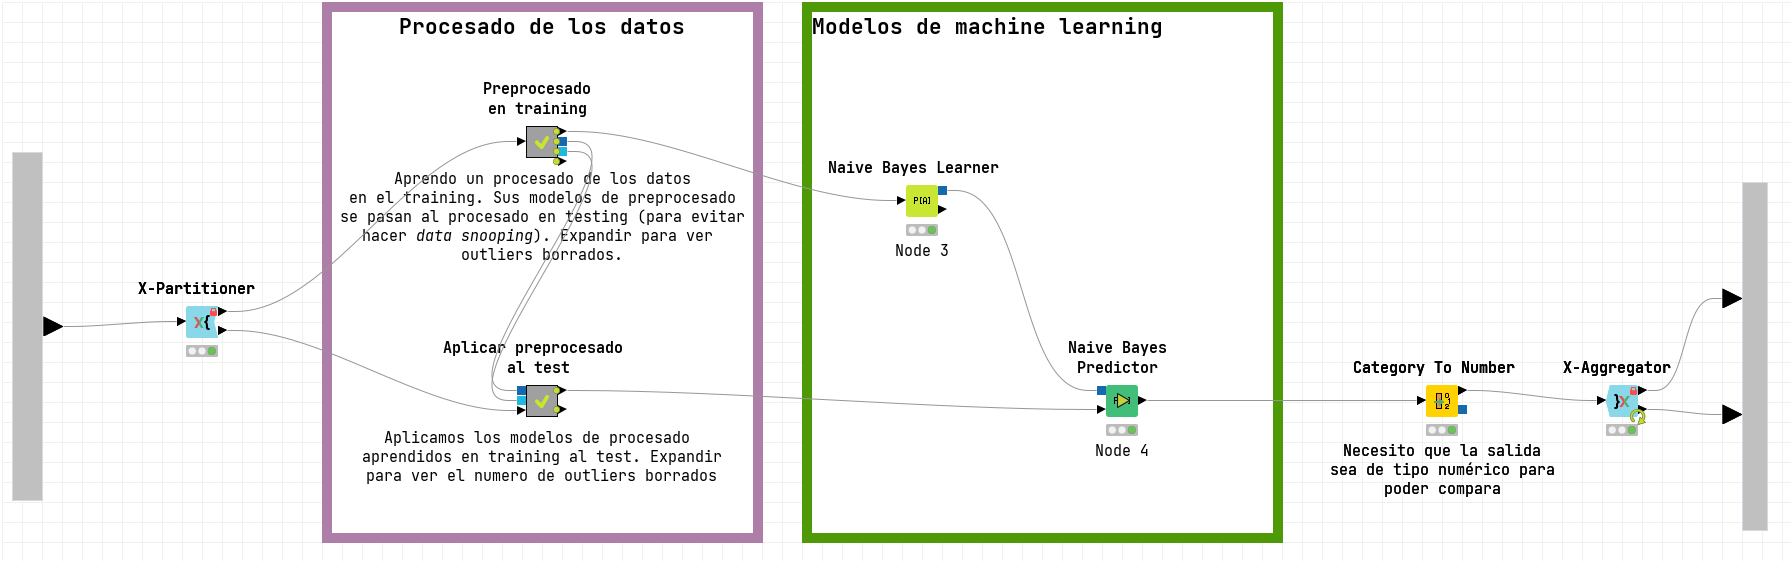
\includegraphics[width = 0.9 \textwidth]{dataset01_cv_naivebayes}
    \caption{Nodo de \emph{Cross Validation} para \emph{Naive Bayes}}
\end{figure}

Terminamos esta sección mostrando el proceso para Random Forest. De nuevo, no realizamos un preprocesado previo general para aplicar el algoritmo, como se muestra a continuación:

\begin{figure}[H]
    \centering
    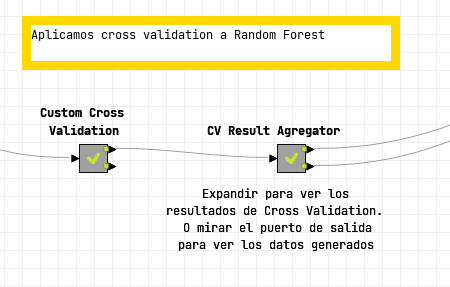
\includegraphics[width = 0.9 \textwidth]{dataset01_cv_pregeneral_randomforest}
    \caption{Preprocesado general previo a probar \emph{Random Forest}. En este caso tampoco estamos realizando ningún tipo de preprocesado previo a \emph{Custom Cross Validation}}
\end{figure}

Y de nuevo, nos encontramos con la misma situación dentro de \emph{Custom Cross Validation}. Simplemente pasamos a variable numérica la salida para que funcione bien el nodo de \lstinline{X-Aggregator}. Mostramos esto en la siguiente figura:

\begin{figure}[H]
    \centering
    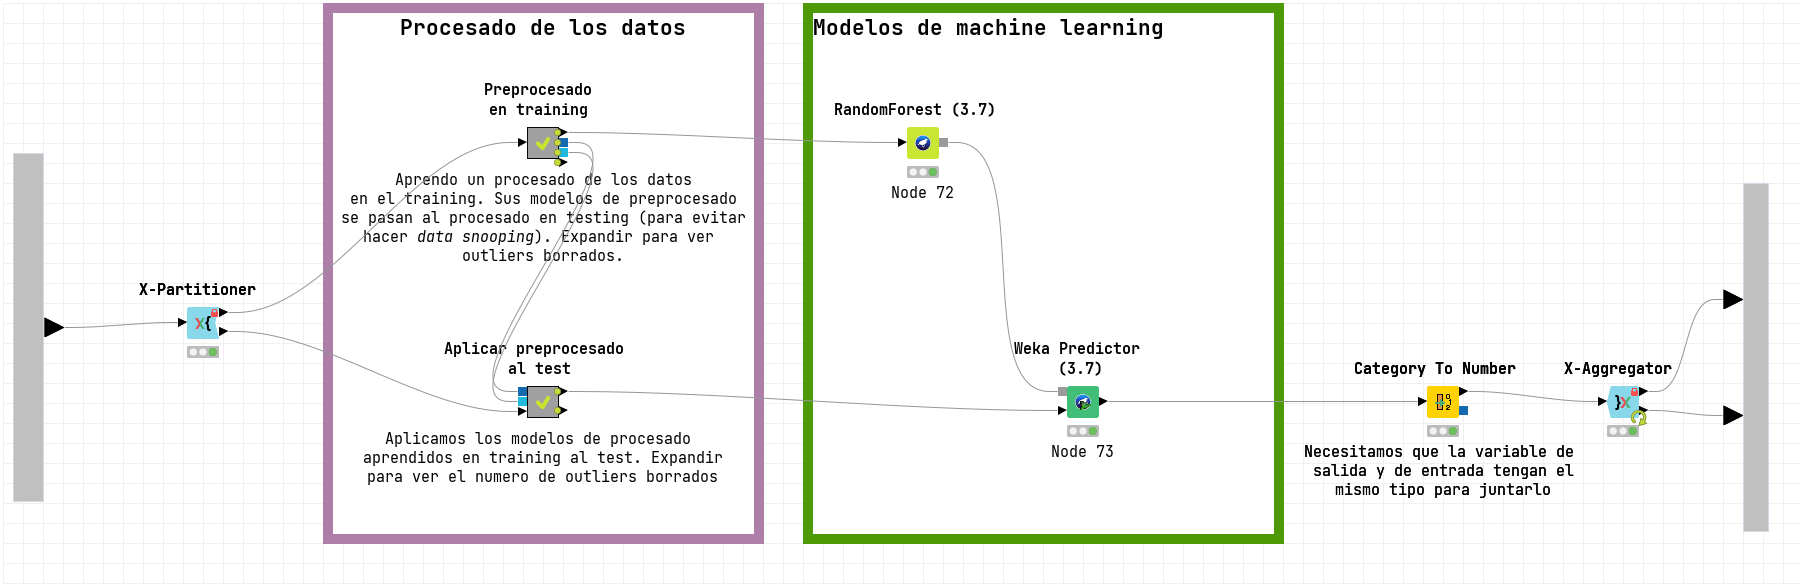
\includegraphics[width = 0.9 \textwidth]{dataset01_cv_randomforest}
    \caption{Nodo de \emph{Cross Validation} para \emph{Random Forest}}
\end{figure}

\pagebreak

\subsubsection{Mostrando los resultados obtenidos}

En primer lugar, mostramos la tabla que resume todos los resultados obtenidos tras el proceso de \emph{Cross Validation}:

\begin{table}[H]
\begin{center}
    \resizebox{1.05\textwidth}{!}{
    \begin{tabular}{|c|c|c|c|c|c|c|c|c|c|c|c|c|}
        \hline
        Algo Name&TP&FP&TN&FN&Recall&Precision&Sensitivity&Specificity&F-measure&AUC&Accuracy&G-Mean\\
        \hline
        Naive Bayes&212&106&247&79&0.73&0.67&0.73&0.70&0.70&0.92&0.71&0.71 \\
        Neural Net&212&42&179&48&0.82&0.83&0.82&0.81&0.82&0.88&0.81&0.81 \\
        Support Vector Machine&6&1&352&285&0.02&0.86&0.02&1.00&0.04&1&0.56&0.14 \\
        Support Vector Machine + Normalization&141&33&332&195&0.42&0.81&0.42&0.91&0.55&1&0.67&0.62 \\
        K-NN&155&161&192&136&0.53&0.49&0.53&0.54&0.51&0.72&0.54&0.54 \\
        AdaBoost&208&102&251&83&0.71&0.67&0.71&0.71&0.69&0.92&0.71&0.71 \\
        Random Forest&215&107&246&76&0.74&0.67&0.74&0.70&0.70&0.92&0.72&0.72 \\
        \hline
    \end{tabular}}
\end{center}
    \caption{Resultados de \emph{Cross Validation}, para los distintos algoritmos estudiados, en el primer \emph{dataset}}
\end{table}

Mostramos ahora una tabla con las medidas de complejidad de cada uno de los algoritmos estudiados:

\begin{table}[H]
\begin{center}
    % \resizebox{1.05\textwidth}{!}{
    \begin{tabular}{|c|c|}
        \hline
        Algo Name & Medida de Complejidad \\
        \hline
        Naive Bayes& 20 valores únicos por atributo \\
        Neural Net & 1 hidden layer, 10 neuronas \\
        Support Vector Machine& Kernel RBF $\sigma = 2.0$ \\
        Support Vector Machine + Normalization& Kernel RBF $\sigma = 2.0$ \\
        K-NN& 10 vecinos \\
        AdaBoost& 10 iteraciones \\
        Random Forest& 50 árboles, profundidad no acotada \\
        \hline
    \end{tabular}
% }
\end{center}
    \caption{Medidas de complejidad de los algoritmos considerados}
\end{table}

\pagebreak

\subsubsection{Mostrando las curvas ROC obtenidas}

En todos los algoritmos, hemos tomado las probabilidades de clasificación, con las que hemos mostrado las curvas ROC para la clase positiva. Estas curvas las mostramos tanto de forma individual como de forma conjunta. Empezamos mostrando la gráfica con todas las curvas ROC agrupadas:

\begin{figure}[H]
    \centering
    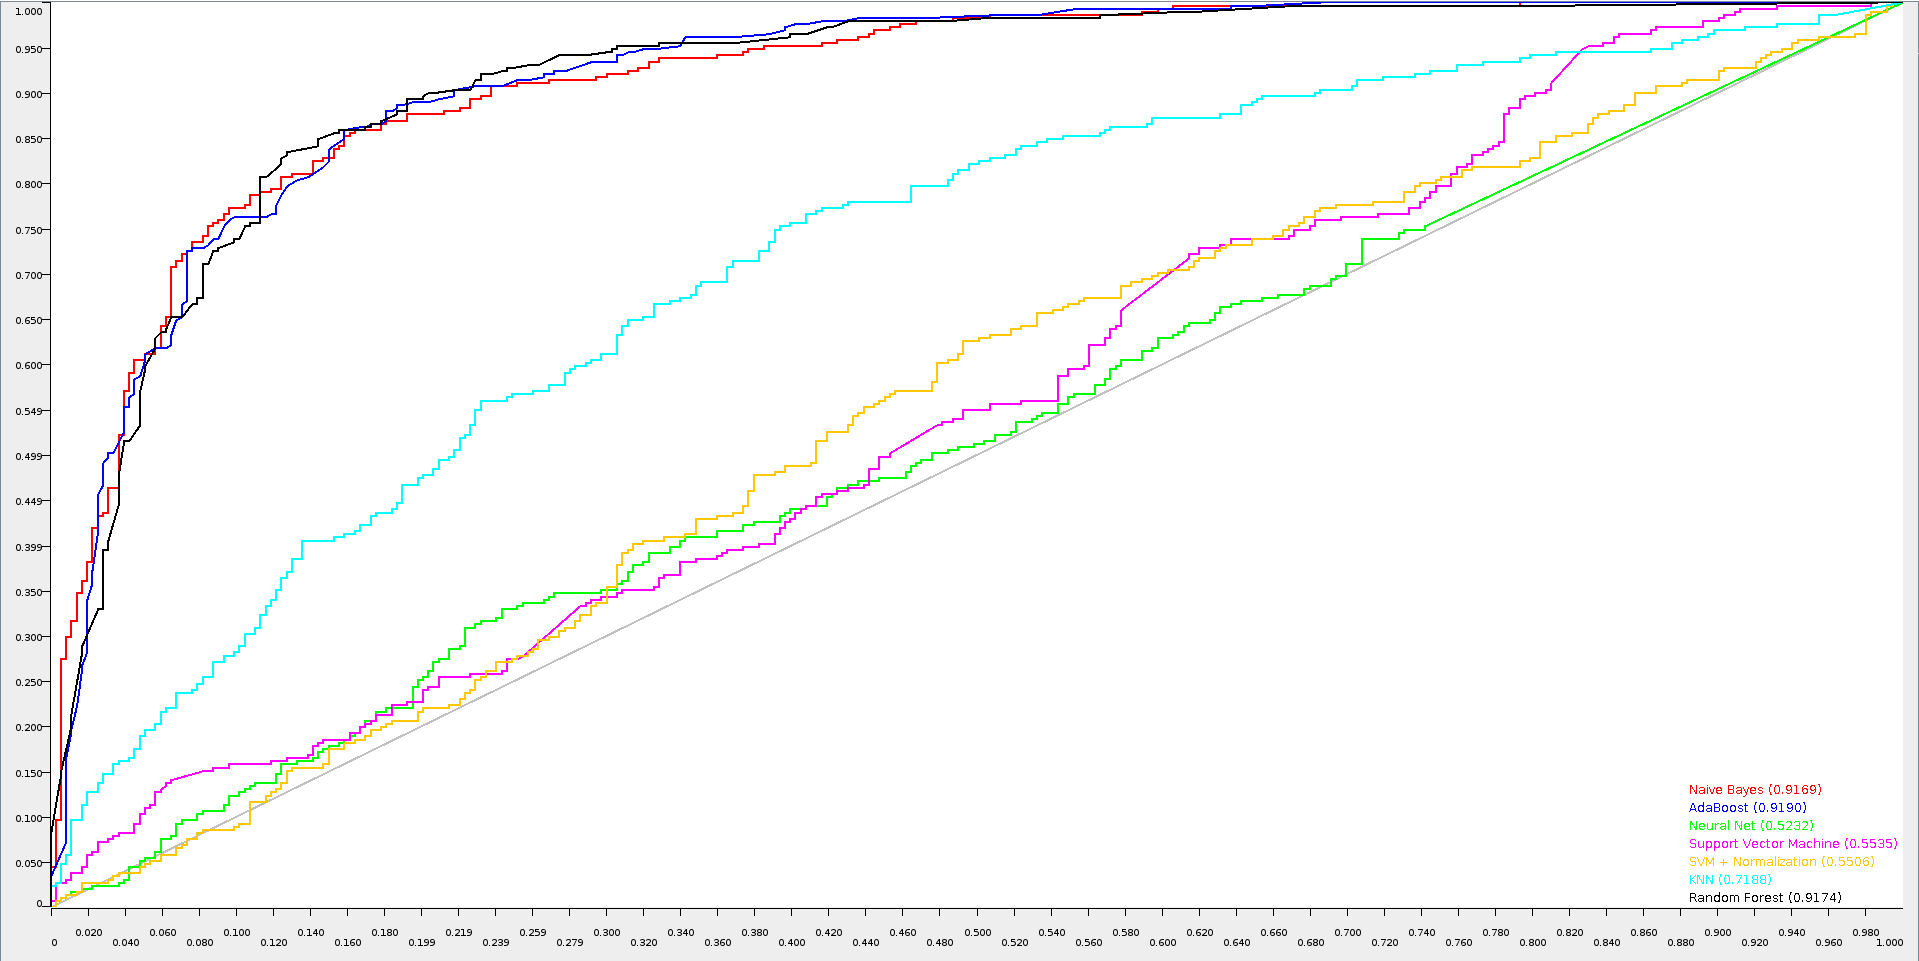
\includegraphics[width = 0.8 \textwidth]{dataset01_allroc}
    \caption{Todas las curvas ROC de los algoritmos estudiados}
    \label{workflow_general:imagen}
\end{figure}

Algunos algoritmos se muestran de forma correcta. Es el caso de Naive Bayes, Random Forest, AdaBoost y K-NN. Los otros tres algoritmos (SVM en sus dos variantes y la red neuronal) se muestran de forma incorrecta. Esto se explica porque estos algoritmos no tratan de la misma forma los \emph{missing values}, en muchos casos ignorándolos. Por tanto, obtenemos dos tipos de tablas que juntar, un tipo con todas las filas originales, y otro tipo de tabla en la que faltan algunas filas. Por tanto la visualización no es correcta. Es por esto que mostramos a continuación todas las curvas de forma individual:

\begin{figure}[H]
    \centering

    \begin{subfigure}[b]{0.4 \textwidth}
        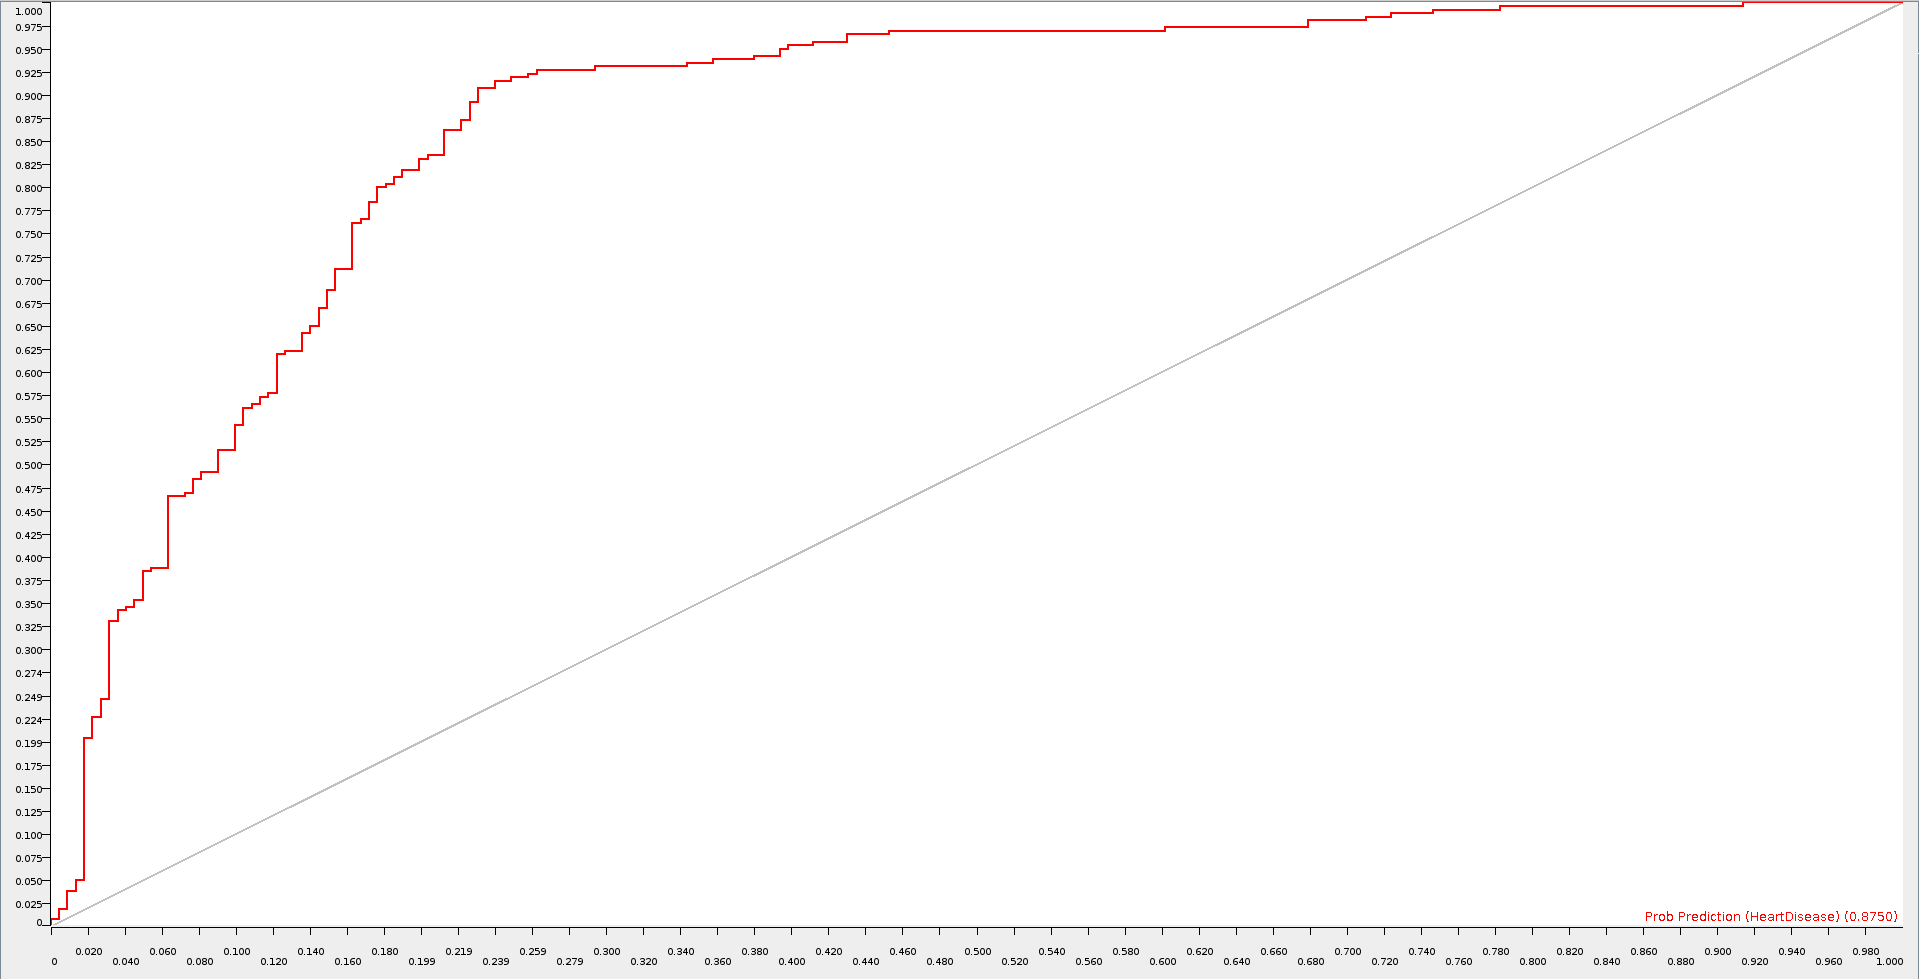
\includegraphics[width = 0.9 \textwidth]{dataset01_roc_nn}
        \caption{Curva ROC para Redes Neuronales}
    \end{subfigure}
    \begin{subfigure}[b]{0.4 \textwidth}
        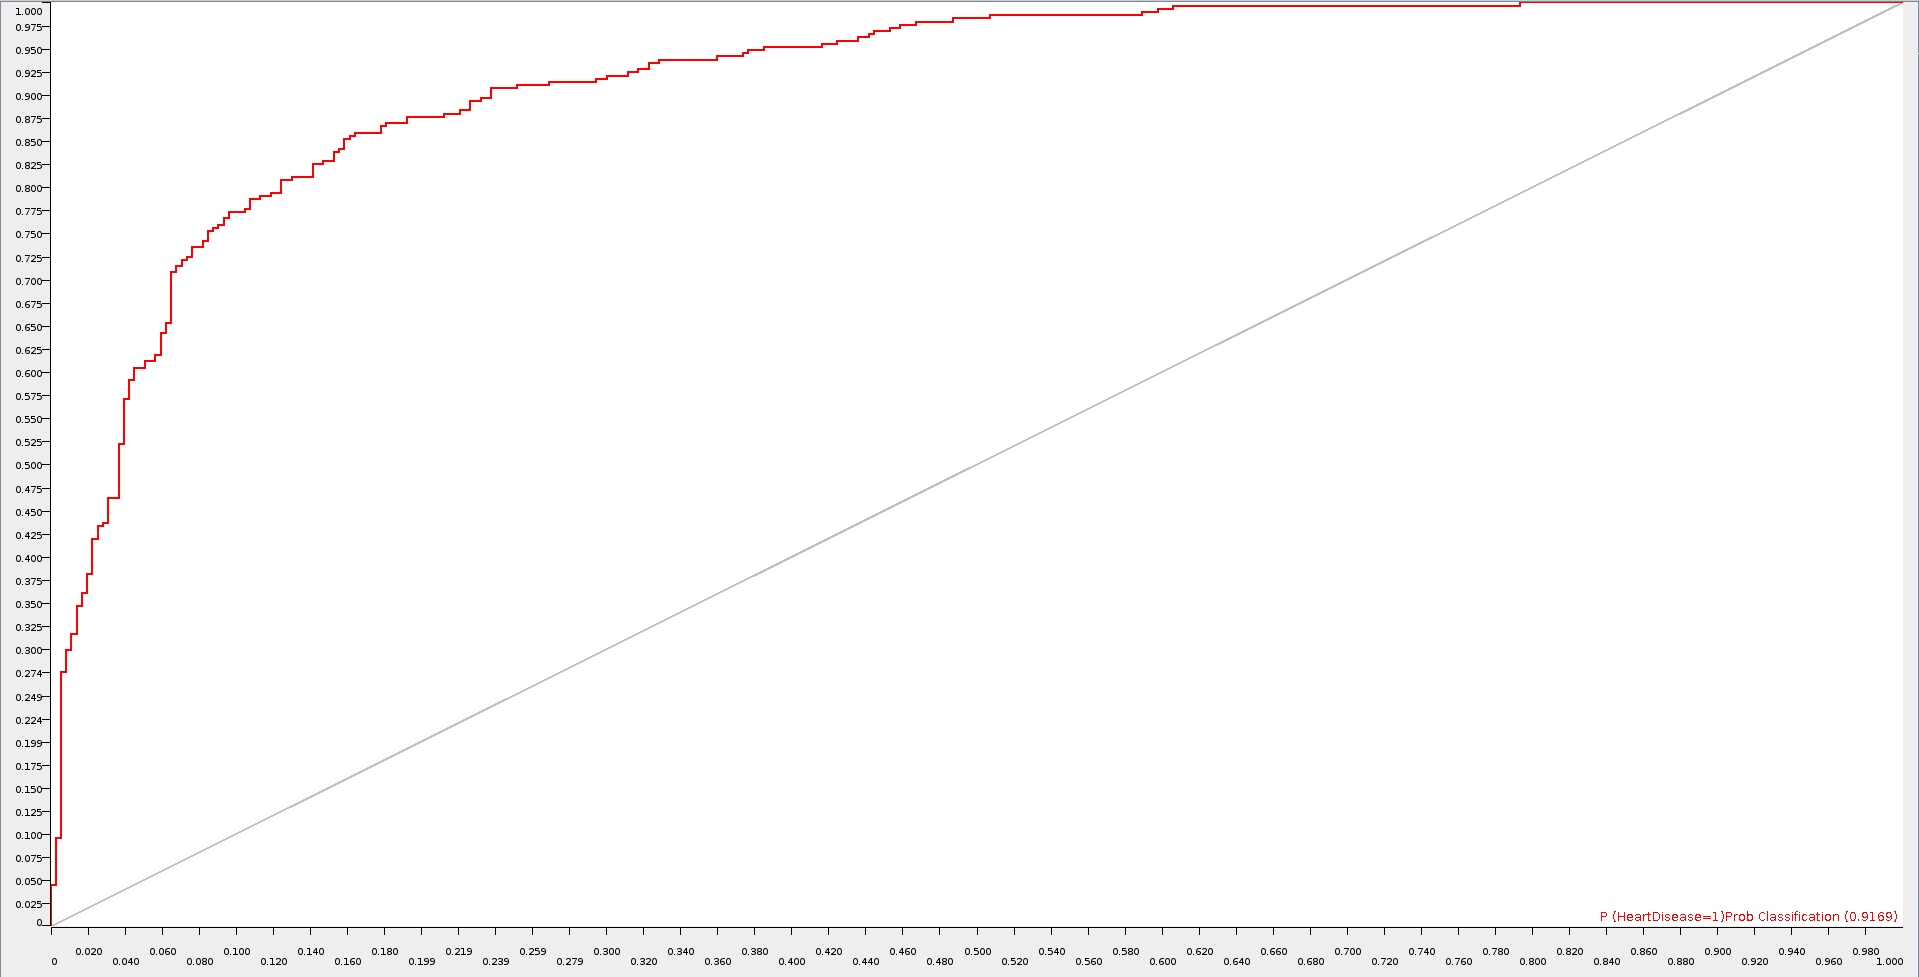
\includegraphics[width = 0.9 \textwidth]{dataset01_roc_naivebayes}
        \caption{Curva ROC para Naive Bayes}
    \end{subfigure}

    \begin{subfigure}[b]{0.4 \textwidth}
        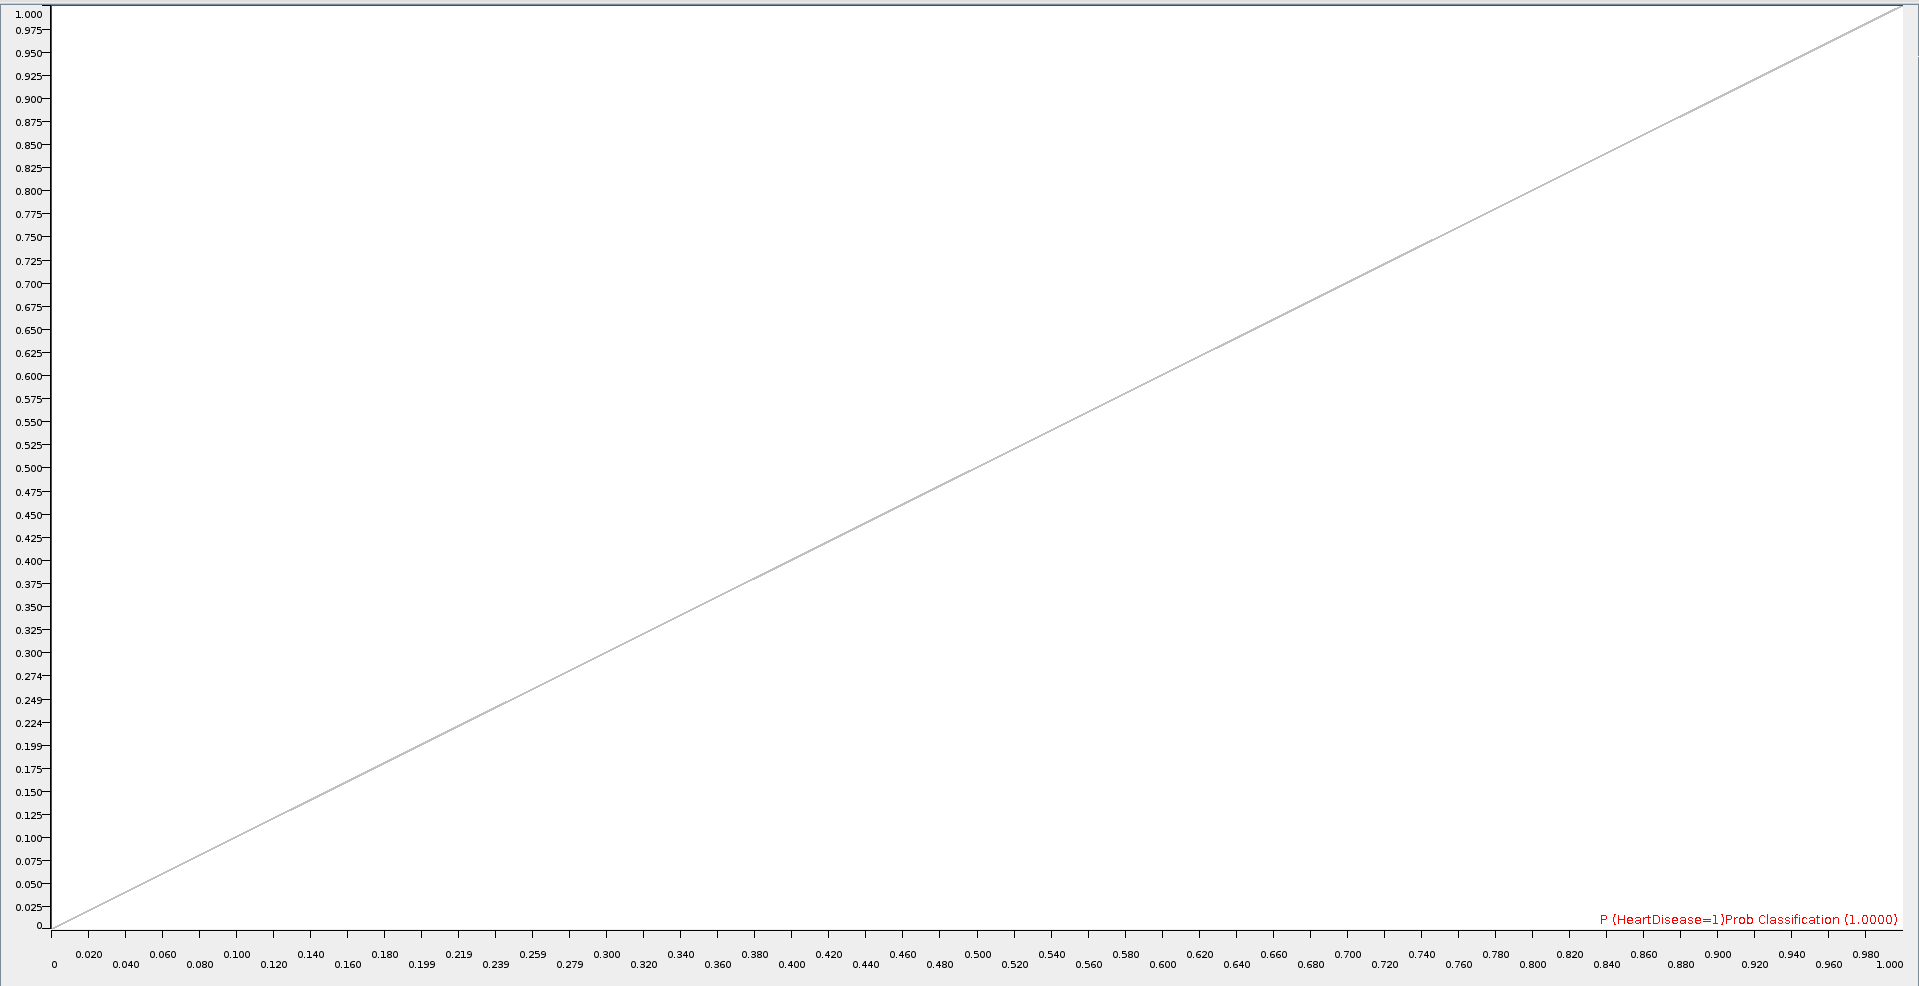
\includegraphics[width = 0.9 \textwidth]{dataset01_roc_svm}
        \caption{Curva ROC para SVM}
    \end{subfigure}
    \begin{subfigure}[b]{0.4 \textwidth}
        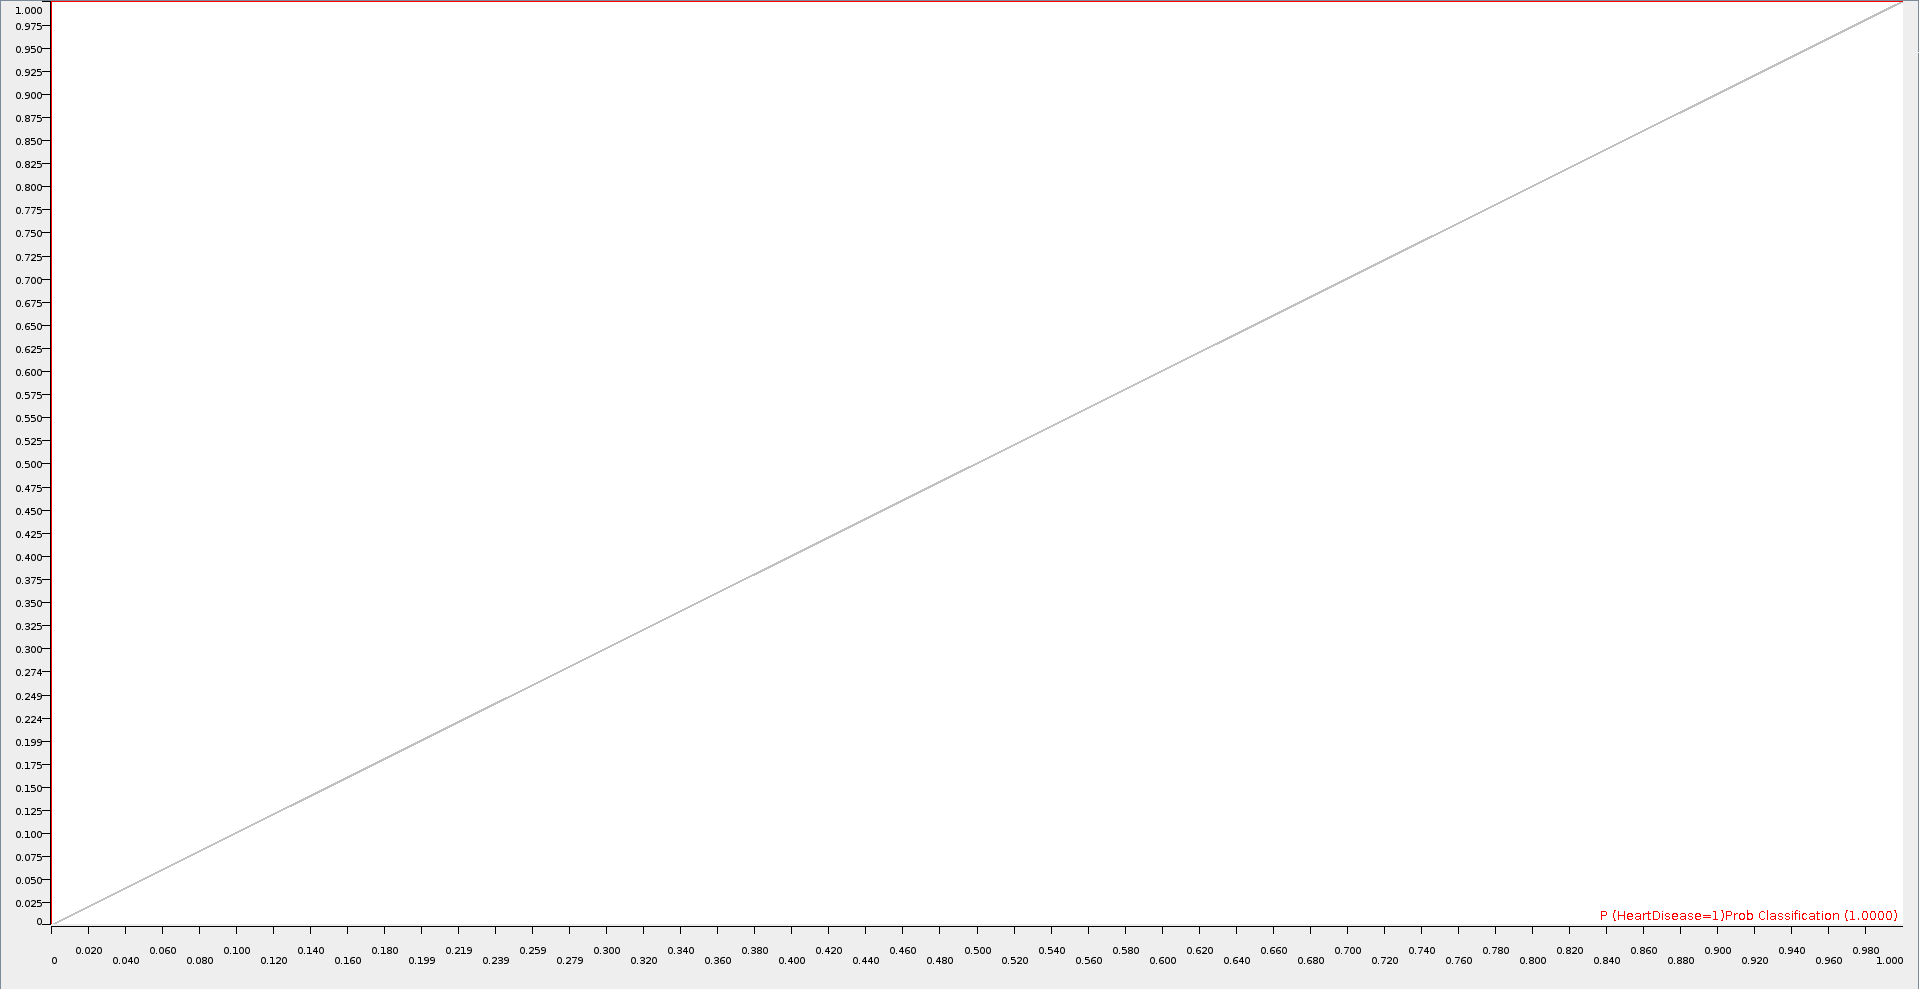
\includegraphics[width = 0.9 \textwidth]{dataset01_roc_svmnormalizacion}
        \caption{Curva ROC para SVM con normalización}
    \end{subfigure}

    \begin{subfigure}[b]{0.4 \textwidth}
        \includegraphics[width = 0.9 \textwidth]{dataset01_roc_knn}
        \caption{Curva ROC para K-NN}
    \end{subfigure}
    \begin{subfigure}[b]{0.4 \textwidth}
        \includegraphics[width = 0.9 \textwidth]{dataset01_roc_randomforest}
        \caption{Curva ROC para Random Fores}
    \end{subfigure}

    \begin{subfigure}[b]{0.4 \textwidth}
        \includegraphics[width = 0.9 \textwidth]{dataset01_roc_adaboost}
        \caption{Curva ROC para Adaboost}
    \end{subfigure}

    \caption{Todas las curvas ROC para el primer \emph{dataset}, mostradas de forma individual}
\end{figure}

Con esta visualización sí que se pueden extraer más conclusiones sobre el comportamiento de los algoritmos, como desarrollaremos más adelante.

\pagebreak

\subsection{Mobile Price Classification} \label{mobile_price_cross_validation:seccion}

% TODO -- tenemos que comentar como hemos hecho la adaptacion multiclase

\subsubsection{\emph{Workflows} empleados para \emph{Cross Validation}} \label{dataset02_decision:seccion}

Como ya hemos comentado previamente, no vamos a mostrar capturas de pantalla de los \emph{workflows} de cada \emph{Custom Cross Validation} para cada algoritmo. Esto pues las diferencias respecto al \emph{dataset} anterior son mínimas. Consideramos, por tanto, que es mucho más interesante que solo mostremos las diferencias con respecto lo desarrollado previamente.

Un \textbf{problema fundamental} con el que nos encontramos es que tenemos un problema de clasificación multiclase. Se nos presentan las siguientes posibles soluciones:

\begin{enumerate}
    \item Trabajar este problema con \lstinline{KNIME}. Para los algoritmos que trabajan directamente con clasificación multiclase, solo hace falta recopilar las métricas y curvas ROC clase por clase. En los algoritmos que no trabajan con multiclase, realizar alguna adaptación (como \emph{One vs All}) usando \emph{loops}
    \item Realizar una adaptación incorrecta pero que simplifica nuestro trabajo. Colapsar las cuatro clases en solo dos clases. Es decir, los datos de la clase 2 tomarlos como datos de la clase 1, y los datos de la clase 4 tomarlos como datos de la clase 3. Con ello tenemos un problema de clasificación binaria que ya hemos trabajado.
    \item Trabajar con \lstinline{KNIME} como lo hemos hecho antes, y solo considerar la clase 1 como clase positiva. Intentar usar directamente los algoritmos sin realizar adaptaciones, y descartar aquellos que no funcionen.
\end{enumerate}

En un primer momento, consideramos la primera posibilidad por ser la más correcta. Sin embargo, suponía demasiada carga de trabajo trabajar las tablas en \lstinline{KNIME}, y no nos daba tiempo. Y más fundamentalmente, no hemos encontrado de realizar la adaptación \emph{One vs All} en \lstinline{KNIME}. Se puede hacer con los nodos de voto y haciendo \emph{loops}, pero en ningún caso hemos conseguido que esto funcione.

La segunda opción la hemos descartado. Quizá sea más correcta (dentro de la gran simplificación que hacemos del problema) que la tercera. Sin embargo, el interés de este \emph{dataset} es precisamente trabajar con un problema multiclase, y con esa aproximación perdemos la oportunidad de realizar todos los análisis respecto a este aspecto.

La tercera opción, que es la que hemos seguido, dista mucho de ser perfecta. Sin embargo, nos permite extraer conclusiones sobre el factor multiclase. Indicaremos así las carencias que tiene \lstinline{KNIME} para trabajar de forma eficiente con problemas multiclase, y los problemas que tienen ciertos algoritmos con clasificación que no sea binaria. Además, también podremos discutir sobre la información que nos dan ciertas métricas respecto a tener más de una clase.

Por tanto, al seguir este proceder, no hemos realizado ningún cambio sustancial en los \emph{workflows} que ya hemos mostrado en \customcite{dataset01_capturas_cv:seccion}.

\pagebreak

\subsubsection{Mostrando los resultados obtenidos}

En primer lugar, mostramos la tabla que resume todos los resultados obtenidos tras el proceso de \emph{Cross Validation}:

\begin{table}[H]
\begin{center}
    \resizebox{1.05\textwidth}{!}{
    \begin{tabular}{|c|c|c|c|c|c|c|c|c|c|c|c|c|}
        \hline
        Algo Name&TP&FP&TN&FN&Recall&Precision&Sensitivity&Specificity&F-measure&AUC&Accuracy&G-Mean\\
        \hline
        Naive Bayes & 283 & 90 & 1064 & 86 & 0.767 & 0.759 & 0.767 & 0.922 & 0.763 & 0.582 & 0.685 & 0.841 \\
        Neural Net & 0 & 789 & 734 & 0 & ?? & 0 & ?? & 0.482 & ??  & 0.995 & 0 & ?? \\
        Support Vector Machine & 0 & 0 & 1145 & 378 & 0 & ??  & 0 & 1 & ??  & 0.488 & 0.247 & 0 \\
        Support Vector Machine + Normalization & 42 & 28 & 1117 & 336 & 0.111 & 0.600 & 0.111 & 0.976 & 0.188 & 0.784 & 0.557 & 0.329 \\
        K-NN & 275 & 118 & 1036 & 94 & 0.745 & 0.700 & 0.745 & 0.898 & 0.722 & 0.599 & 0.734 & 0.818 \\
        AdaBoost & 204 & 537 & 608 & 174 & 0.540 & 0.275 & 0.540 & 0.531 & 0.365 & 0.719 & 0.234 & 0.535 \\
        Random Forest & 266 & 126 & 1028 & 103 & 0.721 & 0.679 & 0.721 & 0.891 & 0.699 & 0.490 & 0.677 & 0.801 \\
        \hline
    \end{tabular}}
\end{center}
    \caption{Resultados de \emph{Cross Validation}, para los distintos algoritmos estudiados, en el segundo \emph{dataset}}
\end{table}

Notar que hay valores marcados con \emph{??}. Ciertos algoritmos no han clasificado ningún valor en la clase positiva o ningún valor en la clase no positiva. Por tanto, en algunas métricas se divide por cero, lo que provoca estos valores \emph{??}.

Mostramos ahora una tabla con las medidas de complejidad de cada uno de los algoritmos estudiados:

\begin{table}[H]
\begin{center}
    % \resizebox{1.05\textwidth}{!}{
    \begin{tabular}{|c|c|}
        \hline
        Algo Name & Medida de Complejidad \\
        \hline
        Naive Bayes& 20 valores únicos por atributo \\
        Neural Net & 1 hidden layer, 10 neuronas \\
        Support Vector Machine& Kernel RBF $\sigma = 3.0$ \\
        Support Vector Machine + Normalization& Kernel RBF $\sigma = 2.0$ \\
        K-NN& 5 vecinos \\
        AdaBoost& 10 iteraciones \\
        Random Forest& 50 árboles, profundidad no acotada \\
        \hline
    \end{tabular}
% }
\end{center}
    \caption{Medidas de complejidad de los algoritmos considerados, en el segundo \emph{dataset}}
\end{table}

En este caso hemos modificado el valor de $\sigma$ para \emph{SVM} no normalizado y el número de vecinos para \emph{K-NN}, respecto el primer \emph{dataset}.

\pagebreak

\subsubsection{Mostrando las curvas ROC obtenidas}

Por la decisión tomada en \customcite{dataset02_decision:seccion}, tenemos algoritmos con resultados catastróficos. Esto hace que la curva \emph{ROC} conjunta muestre comportamiento muy malos, y por ello, no podemos extraer información útil a partir de dicha gráfica conjunta. Por tanto, mostramos directamente las curvas \emph{ROC} individuales:

\begin{figure}[H]
    \centering

    \begin{subfigure}[b]{0.4 \textwidth}
        \includegraphics[width = 0.9 \textwidth]{dataset02_roc_nn}
        \caption{Curva ROC para Redes Neuronales}
    \end{subfigure}
    \begin{subfigure}[b]{0.4 \textwidth}
        \includegraphics[width = 0.9 \textwidth]{dataset02_roc_naivebayes}
        \caption{Curva ROC para Naive Bayes}
    \end{subfigure}

    \begin{subfigure}[b]{0.4 \textwidth}
        \includegraphics[width = 0.9 \textwidth]{dataset02_roc_svm}
        \caption{Curva ROC para SVM}
    \end{subfigure}
    \begin{subfigure}[b]{0.4 \textwidth}
        \includegraphics[width = 0.9 \textwidth]{dataset02_roc_svmnormalizacion}
        \caption{Curva ROC para SVM con normalización}
    \end{subfigure}

    \begin{subfigure}[b]{0.4 \textwidth}
        \includegraphics[width = 0.9 \textwidth]{dataset02_roc_knn}
        \caption{Curva ROC para K-NN}
    \end{subfigure}
    \begin{subfigure}[b]{0.4 \textwidth}
        \includegraphics[width = 0.9 \textwidth]{dataset02_roc_randomforest}
        \caption{Curva ROC para Random Fores}
    \end{subfigure}

    \begin{subfigure}[b]{0.4 \textwidth}
        \includegraphics[width = 0.9 \textwidth]{dataset02_roc_adaboost}
        \caption{Curva ROC para Adaboost}
    \end{subfigure}

    \caption{Todas las curvas ROC para el segundo \emph{dataset}, mostradas de forma individual}
\end{figure}

\pagebreak

\subsection{Bank Marketing}

\subsubsection{\emph{Workflows} empleados para \emph{Cross Validation}}

Para este \emph{dataset} realizamos dos cambios respecto a los \emph{datasets} anteriores:

\begin{enumerate}
    \item \emph{SVM} en sus dos variantes tarda demasiado tiempo en ejecutarse en nuestro ordenador (más de 5h tras haber otorgado a \lstinline{KNIME} toda la potencia disponible en nuestra máquina). Por tanto, usamos el nodo \lstinline{partitioning} para ejecutar y evaluar ambos algoritmos en solo el $15\%$ de los datos.
    \item Tras esta reducción de los ejemplos, \emph{SVM} con normalización no seguía sin ejecutarse en un tiempo razonable. Es por esto que decidimos no ejecutar este algoritmo para este problema, y comentar este hecho en los análisis pertinentes
    \item Aplicamos normalización a \emph{K-NN}. Sin esta normalización el rendimiento obtenido en este modelo es demasiado malo. Esto no nos había pasado hasta este \emph{dataset}, y por tanto no nos habíamos dado cuenta del fallo. Además, decidimos dejar el fallo en los dos \emph{datasets} previos por la posibilidad de análisis que abre dejar este fallo en el \emph{``código''}
\end{enumerate}

El particionado de los datos para aplicar \emph{SVM} en un tiempo razonable, y el borrado de \emph{SVM} con normalización, se muestra en la siguiente captura:

\begin{figure}[H]
    \centering
    \includegraphics[width = 0.8 \textwidth]{dataset03_workflowpca_svm}
    \caption{Particionado de los datos, para que \emph{SVM} en sus dos variantes trabaje con menos datos, y podamos así entrenar y evaluar estos dos modelos en un tiempo razonable. A pesar de esto, \emph{SVM} con normalización no es capaz de ejecutarse en un tiempo razonable. Y por ello, borramos ese modelo}
\end{figure}

Mostramos ahora el proceso de normalización de los datos para mejorar el rendimiento de \emph{K-NN}:

\begin{figure}[H]
    \centering
    \includegraphics[width = 0.8 \textwidth]{dataset03_workflowpca_knnnorm}
    \caption{Normalización de los datos previo a evaluar un modelo \emph{K-NN}}
\end{figure}

\pagebreak

\subsubsection{Mostrando los resultados obtenidos}

Mostramos los resultados obtenidos tras aplicar los distintos nodos de \emph{Custom Cross Validation}:

\begin{table}[H]
\begin{center}
    \resizebox{1.05\textwidth}{!}{
    \begin{tabular}{|c|c|c|c|c|c|c|c|c|c|c|c|c|}
        \hline
        Algo Name&TP&FP&TN&FN&Recall&Precision&Sensitivity&Specificity&F-measure&AUC&Accuracy&G-Mean\\
        \hline
        Naive Bayes & 1668 & 4684 & 26324 & 902 & 0.649 & 0.263 & 0.649 & 0.849 & 0.374 & 0.864 & 0.834 & 0.742 \\
        Neural Net & 529 & 356 & 18886 & 1296 & 0.290 & 0.598 & 0.290 & 0.981 & 0.390 & 0.928 & 0.922 & 0.533 \\
        Support Vector Machine & 0 & 0 & 2918 & 288 & 0 & ?? & 0 & 1 & ?? & 0.843 & 0.910 & 0 \\
        K-NN & 18866 & 1406 & 419 & 376 & 0.980 & 0.931 & 0.980 & 0.230 & 0.955 & 0.879 & 0.915 & 0.474 \\
        AdaBoost & 663 & 522 & 30486 & 1907 & 0.258 & 0.559 & 0.258 & 0.983 & 0.353 & 0.927 & 0.928 & 0.504 \\
        Random Forest & 824 & 582 & 30426 & 1746 & 0.321 & 0.586 & 0.321 & 0.981 & 0.414 & 0.936 & 0.931 & 0.561 \\
        \hline
    \end{tabular}}
\end{center}
    \caption{Resultados de \emph{Cross Validation}, para los distintos algoritmos estudiados, en el tercer \emph{dataset}}
    \label{dataset03_pca_resultados:tabla}
\end{table}

De nuevo, y como nos pasaba en el \emph{dataset} anterior, tenemos ciertos valores no definidos que marcamos con un \emph{??}.

Mostramos ahora una tabla con las medidas de complejidad de cada uno de los algoritmos estudiados:

\begin{table}[H]
\begin{center}
    % \resizebox{1.05\textwidth}{!}{
    \begin{tabular}{|c|c|}
        \hline
        Algo Name & Medida de Complejidad \\
        \hline
        Naive Bayes& 20 valores únicos por atributo \\
        Neural Net & 1 hidden layer, 10 neuronas \\
        Support Vector Machine& Kernel RBF $\sigma = 3.0$ \\
        K-NN& 10 vecinos \\
        AdaBoost& 10 iteraciones \\
        Random Forest& 50 árboles, profundidad no acotada \\
        \hline
    \end{tabular}
% }
\end{center}
    \caption{Medidas de complejidad de los algoritmos considerados, en el tercer \emph{dataset}}
\end{table}

\pagebreak

\subsubsection{Mostrando las curvas \emph{ROC} obtenidas}

De nuevo, la gráfica conjunta es demasiado mala como para extraer información relevante. Y por tanto, de nuevo, mostramos las gráficas individuales:

\begin{figure}[H]
    \centering

    \begin{subfigure}[b]{0.4 \textwidth}
        \includegraphics[width = 0.9 \textwidth]{dataset03_roc_nn}
        \caption{Curva ROC para Redes Neuronales}
    \end{subfigure}
    \begin{subfigure}[b]{0.4 \textwidth}
        \includegraphics[width = 0.9 \textwidth]{dataset03_roc_naivebayes}
        \caption{Curva ROC para Naive Bayes}
    \end{subfigure}

    \begin{subfigure}[b]{0.4 \textwidth}
        \includegraphics[width = 0.9 \textwidth]{dataset03_roc_svm}
        \caption{Curva ROC para SVM}
    \end{subfigure}
    \begin{subfigure}[b]{0.4 \textwidth}
        \includegraphics[width = 0.9 \textwidth]{dataset03_roc_adaboost}
        \caption{Curva ROC para Adaboost}
    \end{subfigure}

    \begin{subfigure}[b]{0.4 \textwidth}
        \includegraphics[width = 0.9 \textwidth]{dataset03_roc_knn}
        \caption{Curva ROC para K-NN}
    \end{subfigure}
    \begin{subfigure}[b]{0.4 \textwidth}
        \includegraphics[width = 0.9 \textwidth]{dataset03_roc_randomforest}
        \caption{Curva ROC para Random Fores}
    \end{subfigure}

    \caption{Todas las curvas ROC para el tercer \emph{dataset}, mostradas de forma individual}
\end{figure}

\pagebreak

\section{Análisis de resultados}

En la anterior sección, \customcite{resultados_brutos:seccion}, hemos mostrados los resultados obtenidos. Estos resultados han sido las tablas con las distintas métricas recolectadas, las medidas de complejidad de los algoritmos, y las distintas curvas ROC obtenidas. En base a esto, y a la siguiente tabla comparativa, realizaremos un análisis de los algoritmos obtenidos:

% TODO -- incluir tabla con las medias de los datos
% TODO -- realizar un análisis de los resultados obtenidos

\pagebreak

\section{Configuración de los algoritmos}

\subsection{Consideraciones iniciales}

Por cada \emph{dataset}, hemos seleccionado dos de los mejores modelos para ese problema, y hemos realizado un ajuste de los parámetros de forma iterativa buscando la máxima eficacia de los modelos considerados. Por tanto, desarrollaremos una sección para cada \emph{dataset} en el que realizaremos este estudio. Añadiremos también una sección para desarrollar algunas conclusiones finales sobre todos los ajustes realizados.

Observar que estamos optimizando la métrica \emph{accuracy}, que como sabemos de teoría, tiene ciertos problemas y no es del todo representativa de la eficacia real de los modelos obtenidos. Sin embargo, esto ha sido así porque, para el nodo \emph{Parameter Optimization Loop End}, tenemos que pasar una métrica por \emph{flow variable}, como es posible hacer con el \emph{scorer}. Sin embargo esto no ha sido posible usando un nodo \emph{math formula}, por lo que nos hemos conformado con ajustar el \emph{accuracy} (mala métrica) a través de un proceso iterativo metódico (buena forma de proceder). En otro \emph{software} sería sencillo cambiar esta optimización para ajustar una mejor medida como \emph{G-Mean} siguiendo la misma filosofía.

En este caso, no estamos usando \emph{Cross Validation} para obtener las métricas. En su lugar, estamos dividiendo el conjunto de datos en 2 particiones, una para \emph{training} ($70\%$) y otra para \emph{test} ($30\%$). Con esto calculamos las métricas sobre el conjunto de \emph{test}. Esta decisión ha sido tomada con el objetivo de reducir los tiempos de cómputo, que ya son elevados por la forma de proceder modificando los valores de los parámetros de forma iterativa.

Al igual que hemos hecho previamente, vamos a ser completamente explícitos en \customcite{optim_dataset01:seccion}, y en los siguientes \emph{datasets}, para evitar ser repetitivos, solo incluiremos las diferencias respecto a lo desarrollado anteriormente y los resultados concretos obtenidos para ese \emph{dataset}. Por ejemplo, solo mostramos todas las capturas de los \emph{workflows} en \customcite{optim_dataset01:seccion}.

\pagebreak

\subsection{\emph{Heart Failure Prediction}} \label{optim_dataset01:seccion}

Para este \emph{dataset}, elegimos optimizar \emph{Random Forest} y la red neuronal simple. Mostramos el \emph{workflow} global en el que ajustamos los dos modelos:

\begin{figure}[H]
    \centering
    \includegraphics[width = 0.8 \textwidth]{dataset01_optim_gobal}
    \caption{\emph{Workflow} global para ajustar los dos algoritmos elegidos}
\end{figure}

Ahora mostramos la optimización que realizamos, en cada uno de los dos modelos:

\begin{figure}[H]
    \centering
    \includegraphics[width = 0.8 \textwidth]{dataset01_optim_first}
    \caption{\emph{Workflow} para ajustar \emph{Random Forest}}
\end{figure}

\begin{figure}[H]
    \centering
    \includegraphics[width = 0.8 \textwidth]{dataset01_optim_second}
    \caption{\emph{Workflow} para ajustar Redes Neuronales Simples}
\end{figure}

En ambos casos estamos usando el nodo \lstinline{Parameter Optimization Loop}. Para trabajar con este nodo, especificamos los parámetros que queremos optimizar, los rangos y los \emph{steps} que tomar. Además, optimizamos usando la opción de fuerza bruta, pues estamos probando con pocas combinaciones de parámetros, por lo que nos podemos permitir este proceder. Una vez hecho esto, especificamos a nuestro modelo que use en cada iteración estos parámetros, usando para ello \emph{flow variables}.

Una vez mostrado esto, a continuación tenemos las tablas obtenidas del proceso de optimización:

\begin{table}[H]
\begin{center}
    \begin{tabular}{|c|c|}
        \hline
        Number of trees&Objective value \\
        \hline
        10&0.837               \\
        20&0.841               \\
        30&0.859               \\
        40&0.862               \\
        50&0.859               \\
        60&0.848               \\
        70&0.851               \\
        80&0.855                \\
        90&0.859               \\
        100&0.862              \\
        110&0.862              \\
        120&0.859              \\
        130&0.862              \\
        140&0.862              \\
        \textbf{150}&\textbf{0.866}              \\
        \hline
    \end{tabular}
\end{center}
    \caption{Optimización para \emph{Random Forest}, ajustando el número de árboles}
\end{table}

En este caso, vemos que el \emph{accuracy} crece de forma más o menos monótona conforme aumentamos el número de árboles que conforman el bosque. Por tanto, obtenemos el mejor resultado en el valor más alto de número de árboles, y lo lógico sería continuar aumentando dicho valor y ver cómo evoluciona la métrica estudiada. Pero como ya hemos comentado, estamos usando como métrica el \emph{accuracy}, que no es una métrica del todo fiable, y por tanto decidimos no aumentar este valor en \emph{pro} de obtener un modelo más simple y, por tanto, potencialmente mucho más generalizable.

\begin{table}[H]
\begin{center}
    \begin{tabular}{|c|c|c|}
        \hline
        Neurons per h.layer&Hidden Layers&Objective value \\
        \hline
        10&1&0.446 \\
        20&1&0.446 \\
        \textbf{30}&\textbf{1}&\textbf{0.554} \\
        40&1&0.446 \\
        50&1&0.511 \\
        60&1&0.522 \\
        70&1&0.551 \\
        80&1&0.464 \\
        90&1&0.446 \\
        100&1&0.554 \\
        10&2&0.554 \\
        20&2&0.551 \\
        30&2&0.554 \\
        40&2&0.446 \\
        50&2&0.446 \\
        60&2&0.446 \\
        70&2&0.406 \\
        80&2&0.554 \\
        90&2&0.388 \\
        100&2&0.554 \\
        10&3&0.446 \\
        20&3&0.493 \\
        30&3&0.446 \\
        40&3&0.554 \\
        50&3&0.446 \\
        60&3&0.554 \\
        70&3&0.471 \\
        80&3&0.554 \\
        90&3&0.446 \\
        100&3&0.446 \\
        \hline

    \end{tabular}
\end{center}
    \caption{Optimización para \emph{Redes Neuronales Simples}, ajustando el número de capas ocultas y el número de neuronas por capa oculta}
\end{table}

En este caso, obtenemos los mejores resultados para 30 neuronas y una única capa oculta. Esto lo que nos muestra es que los mejores resultados no los estamos obteniendo con un modelo más potente, sino con uno más simple con menor capacidad de sobreajustar.

Hay que tener en cuenta que las redes neuronales de \lstinline{KNIME} son muy simples, y dan muy poco de sí. Para poder trabajar con modelos más potentes de redes neuronales (más capas ocultas con más neuronas por capa), necesitamos \textbf{técnicas de regularización}. Por ejemplo, no podemos establecer una regularización tipo \emph{weight decay}. Tampoco podemos usar \emph{dropout} para paliar el sobreajuste. Y con ello, es lógico que modelos más simples generen mejores resultados en \emph{test}, por su menor capacidad de sobreajuste.

Además, por problemas con el nodo \lstinline{Parameter Optimization Loop}, no podemos tratar los \emph{missing values} ni normalizar las variables sin que esto provoque fallos que no sabemos resolver. Por esto, obtenemos resultados peores que los mostrados previamente para \emph{Custom Cross Validation}. Sin embargo, la metodología y el ajuste es correcto. Sería cuestión de encontrar el fallo que nos da \lstinline{KNIME} y solucionarlo, o emplear otro \emph{Software} para este ajuste.

\pagebreak

\subsection{Mobile Price Classification}

Para este \emph{dataset}, elegimos optimizar \emph{Random Forest} por los buenos resultados que nos ha dado, y \emph{K-NN}. Tanto el \emph{workflow} global como el \emph{workflow} para \emph{Random Forest} no han cambiado sustancialmente, así que no mostramos capturas de pantalla para estos dos \emph{workflows}. El \emph{workflow} para \emph{K-NN} se muestra en la siguiente figura:

\begin{figure}[H]
    \centering
    \includegraphics[width = 0.8 \textwidth]{dataset02_optim_knn}
    \caption{\emph{Workflow} para ajustar \emph{K-NN}}
\end{figure}

Mostramos la tabla obtenida en la optimización para \emph{Random Forest}:

\begin{table}[H]
\begin{center}
    \begin{tabular}{|c|c|}
        \hline
        Number of trees & Objective value \\
        \hline
        10 & 0.805 \\
        20 & 0.843 \\
        30 & 0.872 \\
        \textbf{40} & \textbf{0.877} \\
        50 & 0.870 \\
        60 & 0.868 \\
        70 & 0.867 \\
        80 & 0.868 \\
        90 & 0.865 \\
        100 & 0.875 \\
        110 & 0.873 \\
        120 & 0.875 \\
        130 & 0.873 \\
        140 & 0.868 \\
        150 & 0.870 \\
        \hline
    \end{tabular}
\end{center}
    \caption{Optimización para \emph{Random Forest}, ajustando el número de árboles}
\end{table}

Obtenemos los mejores resultados con una cantidad de árboles por cada \emph{forest} modesta, por debajo del valor por defecto que nos da \lstinline{KNIME}. A diferencia del \emph{dataset} anterior, esta vez no tenemos ese crecimiento monótono en el \emph{accuracy}, y para este caso, queda claro que en ocasiones es mejor un modelo más simple, por tanto menos potente, pero con mejor capacidad de generalización.

Mostramos ahora los resultados para la optimización de \emph{K-NN}:

\begin{table}[H]
\begin{center}
    \begin{tabular}{|c|c|}
        \hline
        Number of neighbours & Objective value \\
        \hline
        1 & 0.908 \\
        2 & 0.908 \\
        3 & 0.923 \\
        4 & 0.925 \\
        5 & 0.933 \\
        6 & 0.937 \\
        7 & 0.945 \\
        8 & 0.940 \\
        9 & 0.945 \\
        10 & 0.942 \\
        11 & 0.943 \\
        12 & 0.947 \\
        13 & 0.947 \\
        \textbf{14} & \textbf{0.948} \\
        15 & 0.947 \\
        \hline
    \end{tabular}
\end{center}
    \caption{Optimización para \emph{K-NN}, ajustando el número de vecinos considerados para la clasificación}
    \label{dataset02_optim_knn:tabla}
\end{table}

En este caso, estamos ajustando el número de vecinos considerados. Al aumentar este parámetro, no estamos aumentando la complejidad del modelo. Estamos aumentando la regularización que aplica al modelo. Al considerar más vecinos, suavizamos las fronteras generadas, y por tanto reducimos algo la capacidad de sobreajuste de nuestro modelo.

Con ello, estamos viendo que nuestro modelo se beneficia enormemente de la regularización aplicada. Regularización que, en general, hemos echado de menos en las herramientas que \lstinline{KNIME} pone a nuestra disposición.

Además, cabe resaltar los buenos resultados que obtenemos en \emph{accuracy}. Al tener cuatro clases perfectamente balanceadas, este buen \emph{accuracy} no puede explicarse por un clasificado constante o algún problema de esta índole. Y por tanto, podemos asegurar que estamos obteniendo un modelo de muy buen rendimiento.

\pagebreak

\subsection{Bank Marketing}

En este \emph{dataset} elegimos optimizar los parámetros de los modelos \emph{Random Forest} y \emph{Neural Net}. Ambos modelos han obtenido resultados muy buenos que queremos ajustar al máximo. Ambos modelos ya han sido optimizados previamente, así que mostramos directamente los resultados sin mostrar las capturas de pantalla de los \emph{workflows}. Empezamos con \emph{Random Forest}:

\begin{table}[H]
\begin{center}
    \begin{tabular}{|c|c|}
        \hline
        Number of trees & Objective value \\
        \hline
        10 & 0.890 \\
        20 & 0.890 \\
        30 & 0.891 \\
        40 & 0.891 \\
        50 & 0.891 \\
        60 & 0.891 \\
        70 & 0.891 \\
        80 & 0.891 \\
        90 & 0.891 \\
        100 & 0.892 \\
        110 & 0.892 \\
        120 & 0.892 \\
        130 & 0.892 \\
        \textbf{140} & \textbf{0.892} \\
        150 & 0.892 \\
        \hline
    \end{tabular}
\end{center}
    \caption{Optimización para \emph{Random Forest}, ajustando el número de árboles}
\end{table}

En este caso, obtenemos un comportamiento curioso. Apenas estamos afectando al \emph{accuracy} modificando los parámetros en el rango en el que nos movemos. Esto puede estar ocasionado por dos motivos:

\begin{itemize}
    \item Como ya hemos comentado repetidas veces, la medida \emph{accuracy} no es del todo representativa, y se ve muy afectada por problemas como el desbalanceo de clases (que en nuestro \emph{dataset} es crítico)
    \item Los rangos de valores son muy pequeños como para que generen una diferencia notable
\end{itemize}

Sin embargo, sabiendo que nuestro \emph{dataset} tiene un importante desbalanceo, nos inclinamos más por la primera hipótesis.

Mostramos ahora los resultados para la optimización de redes neuronales:

\begin{table}[H]
\begin{center}
    \begin{tabular}{|c|c|c|}
        \hline
        Neurons per layer & Hidden Layers & Objective value \\
        \hline
        10 & 1 & 0.914 \\
        30 & 1 & 0.914 \\
        50 & 1 & 0.914 \\
        10 & 2 & 0.914 \\
        30 & 2 & 0.915 \\
        50 & 2 & 0.915 \\
        10 & 3 & 0.913 \\
        30 & 3 & 0.915 \\
        50 & 3 & 0.912 \\

        \hline
    \end{tabular}
\end{center}
    \caption{Optimización para \emph{Redes Neuronales}, ajustando el número de capas ocultas y el número de neuronas por capa}
\end{table}

Aquí también obtenemos el mismo comportamiento. Esto reafirma nuestra sospecha de que el desbalanceo de las clases está dominando la métrica de \emph{accuracy}. Gracias a esto, sabemos que los resultados obtenidos en \customcite{dataset03_pca_resultados:tabla}, en lo que a \emph{accuracy} se refiere, son demasiado optimistas.

\pagebreak

\subsection{Conclusiones finales}

% TODO -- hacer estas conclusiones con las configuraciones de los cuatro algoritmos

\pagebreak

\section{Procesado de datos}

\subsection{Consideraciones iniciales}

Desarrollaremos distintos apartados para cada uno de los \emph{datasets}. En vista de los análisis previos para cada \emph{dataset}, tomaremos ciertas decisiones de procesado buscando mejorar el rendimiento de los modelos planteados. Compararemos dicho rendimiento antes y después del procesado, lo que nos permitirá extraer ciertas conclusiones sobre la técnica empleada, sobre el comportamiento de los algoritmos o sobre el problema en sí.

\subsection{\emph{Heart Failure Prediction}} \label{dataset01_procesado_datos:seccion}

Como hemos estudiado en \customcite{dataset01_correlaciones:imagen}, tenemos variables que están muy correladas entre sí. Así que para mejorar este \emph{dataset}, decidimos borrar algunas variables que estén altamente correladas con otras, para ver si conseguimos obtener mejores resultados o, al menos, mantener el mismo rendimiento con menos variables, y por tanto, con modelos más sencillos.

Podríamos haber aplicado otras técnicas. \emph{PCA} ya se demostró poco efectivo (al menos con dos dimensiones) en el análisis exploratorio de datos, pues no proporcionaba una buena distribución de datos. Además tenemos muy pocas variables como para necesitar un método automático de reducción de dimensionalidad (es factible seleccionar las variables manualmente). Tampoco tenemos un desbalanceo excesivo de las clases como para aplicar una técnica como \emph{SMOTE}. Son estas las razones por las que nos decantamos por un procesado de los datos tan básico de los datos (que ya de por sí son básicos).

Este procesado de los datos se realiza del siguiente modo:

\begin{figure}[H]
    \centering
    \includegraphics[width = 0.8 \textwidth]{dataset01_extra_general}
    \caption{\emph{Workflow} de más alto nivel para el procesado de los datos}
\end{figure}

Mostramos el contenido de este nodo:

\begin{figure}[H]
    \centering
    \includegraphics[width = 0.8 \textwidth]{dataset01_extra_concreto}
    \caption{\emph{Workflow} de más alto nivel para el procesado de los datos}
\end{figure}

En este nodo nos quedamos solo con las variables \lstinline{MaxHR}, \lstinline{ExerciseAngina}, \lstinline{Oldpeak}, \lstinline{ST_Slope} y la variable de salida (decisión justificada por lo que comentábamos en el \emph{EDA} para este \emph{dataset}).

Además, tenemos que adaptar los nodos de \emph{Custom Cross Validation}. Como no estamos usando la variable \lstinline{Cholesterol}, no tenemos que crear los \emph{missing values}, porque ya no tenemos. Este es el cambio que realizamos en todos los nodos de \emph{Custom Cross Validation}.

Los resultados obtenidos tras aplicar \emph{Cross Validation} tras esta transformación son los siguientes:

\begin{table}[H]
\begin{center}
    \resizebox{1.05\textwidth}{!}{
    \begin{tabular}{|c|c|c|c|c|c|c|c|c|c|c|c|c|}
        \hline
        Algo Name & TruePositives & FalsePositives & TrueNegatives & FalseNegatives & Recall & Precision & Sensitivity & Specificity & F-measure & Area Under Curve & Accuracy & G-Mean \\
        \hline
        Naive Bayes & 328 & 135 & 314 & 140 & 0.701 & 0.708 & 0.701 & 0.699 & 0.705 & 0.559 & 0.700 & 0.700 \\
        Neural Net & 431 & 86 & 324 & 76 & 0.850 & 0.834 & 0.850 & 0.790 & 0.842 & 0.880 & 0.823 & 0.820 \\
        Support Vector Machine & 421 & 102 & 308 & 86 & 0.830 & 0.805 & 0.830 & 0.751 & 0.817 & 1 & 0.795 & 0.790 \\
        Support Vector Machine + Normalization & 429 & 93 & 317 & 78 & 0.846 & 0.822 & 0.846 & 0.773 & 0.834 & 1 & 0.814 & 0.809 \\
        K-NN & 151 & 268 & 142 & 356 & 0.298 & 0.360 & 0.298 & 0.346 & 0.326 & 0.828 & 0.320 & 0.321 \\
        AdaBoost & 388 & 87 & 362 & 80 & 0.829 & 0.817 & 0.829 & 0.806 & 0.823 & 0.565 & 0.818 & 0.818 \\
        Random Forest & 314 & 128 & 321 & 154 & 0.671 & 0.710 & 0.671 & 0.715 & 0.690 & 0.576 & 0.692 & 0.693 \\
        \hline
    \end{tabular}}
\end{center}
    \caption{Resultados de \emph{Cross Validation}, para los distintos algoritmos estudiados, en el primer \emph{dataset}, tras realizar la selección de variables}
    \label{dataset01_procesado_resultados:seccion}
\end{table}

Aunque ya hemos mostrado esta tabla previamente, mostramos por claridad la tabla de \emph{Cross Validation} obtenida sin el procesado de los datos, para que sea más sencillo realizar la comparación:

\begin{table}[H]
\begin{center}
    \resizebox{1.05\textwidth}{!}{
    \begin{tabular}{|c|c|c|c|c|c|c|c|c|c|c|c|c|}
        \hline
        Algo Name&TP&FP&TN&FN&Recall&Precision&Sensitivity&Specificity&F-measure&AUC&Accuracy&G-Mean\\
        \hline
        Naive Bayes&212&106&247&79&0.73&0.67&0.73&0.70&0.70&0.92&0.71&0.71 \\
        Neural Net&212&42&179&48&0.82&0.83&0.82&0.81&0.82&0.88&0.81&0.81 \\
        Support Vector Machine&6&1&352&285&0.02&0.86&0.02&1.00&0.04&1&0.56&0.14 \\
        Support Vector Machine + Normalization&141&33&332&195&0.42&0.81&0.42&0.91&0.55&1&0.67&0.62 \\
        K-NN&155&161&192&136&0.53&0.49&0.53&0.54&0.51&0.72&0.54&0.54 \\
        AdaBoost&208&102&251&83&0.71&0.67&0.71&0.71&0.69&0.92&0.71&0.71 \\
        Random Forest&215&107&246&76&0.74&0.67&0.74&0.70&0.70&0.92&0.72&0.72 \\
        \hline
    \end{tabular}}
\end{center}
    \caption{Resultados de \emph{Cross Validation}, para los distintos algoritmos estudiados, en el primer \emph{dataset}, \textbf{sin aplicar el procesado de datos}}
    \label{dataset01_sin_procesado_resultados:seccion}
\end{table}

\subsubsection{Conclusiones} \label{dataset01_procesado_datos_conclusiones:seccion}

En base a las dos tablas de resultados anteriores, \customcite{dataset01_procesado_resultados:seccion} y \customcite{dataset01_sin_procesado_resultados:seccion}, realizamos el siguiente análisis.

Nos fijaremos en la métrica \emph{G-Mean}, pues es más informativa que le \emph{accuracy}, como ya hemos señalado varias veces a lo largo de esta memoria. En general hemos mejorado significativamente esta métrica quedándonos con menos columnas en comparación a los resultados sin este preprocesado de datos. Esto es claro pues pasamos de tener un \emph{G-Mean} medio de $0.6071$ a tener un \emph{G-Mean} medio de $0.7072$. Por tanto, \textbf{mejoramos el rendimiento generando modelos más sencillos}.

Nos fijamos ahora en las diferencias algoritmo a algoritmo:

\begin{table}[H]
\begin{center}
    \begin{tabular}{|c|c|}
        \hline
        Algo Name & $procesado - sin\_procesar$ \\
        \hline
        Naive Bayes& -0.010 \\
        Neural Net& 0.010 \\
        SVM& 0.650 \\
        SVM Norm& 0.189 \\
        KNN& -0.219 \\
        Adaboost& 0.108 \\
        Random Forest& -0.027 \\
        \hline
    \end{tabular}
\end{center}
    \caption{Tabla con las diferencias algoritmo a algoritmo, rendimiento del algoritmo tras el procesado menos el rendimiento algoritmo sin el procesado. El rendimiento es \emph{G-Mean}}
\end{table}

Cuando el algoritmo pierde rendimiento, este empeoramiento es muy pequeño (la peor diferencia es $\approx -0.22$). Por tanto podemos decir que, en esos casos estamos manteniendo el rendimiento con modelos más sencillos. Las mejoras, sin embargo, son más grandes (prácticamente el triple de grandes que los empeoramientos, llegando a $\approx 0.65$). Y todo esto teniendo en cuenta que estamos trabajando con un \emph{dataset} mucho más pequeño y, por tanto, generando modelos mucho más simples, por tanto mucho más generalizables y, cuando el algoritmo lo permite, modelos muchos más interpretables.

El algoritmo más perjudicado ha sido \emph{K-NN}. Esto puede ser debido a que, a diferencia de lo que estamos haciendo más adelante, no estamos normalizando los datos de entrada. Por tanto es más sensible a diferencias de escala en las variables. Y al tener menos variables, este efecto es mucho más crítico. Además, al ser un algoritmo que considera información de forma local, al estar quitando variables en las que mirar en la vecindad, es un algoritmo que pierde mucha información por este procesado.

El algoritmo más beneficiado ha sido \emph{SVM} sin normalización. Es destacable que \emph{SVM} con normalización no se haya beneficiado tanto. Por tanto, y como comentábamos para \emph{K-NN}, las distintas escalas de las variables han tenido mucho que ver en este resultado. Creemos que \emph{SVM} sin normalización estaba sufriendo demasiado por diferencias en escala de alguna de las variables que hemos eliminado. Al eliminar estas variables problemáticas, hemos conseguido que el algoritmo tenga mucho mayor rendimiento.

A pesar de esto último, no olvidar que \emph{SVM} con normalización también se ve beneficiado del procesado. Por tanto, además de haber eliminado variables problemáticas para \emph{SVM} sin normalizar, el procesado es en sí mismo beneficioso para el rendimiento de estos modelos.

\pagebreak

\subsection{Mobile Price Classification}

Como hemos comentado en \customcite{dataset02_eda:seccion}, aplicar \emph{PCA} resultando en solo dos variables de entrada parecía muy prometedor. Así que hemos aplicado esto a nuestro \emph{dataset}, y luego hemos comparado con el rendimiento de un algoritmo en concreto.

La estructura general se muestra en el siguiente \emph{workflow}:

\begin{figure}[h]
    \centering
    \includegraphics[width = 0.8 \textwidth]{dataset02_bonus_general}
    \caption{\emph{Workflow} general aplicado para el procesado de datos}
\end{figure}

Aplicamos \emph{PCA} de la forma correcta. Para ello separamos en \emph{training} y \emph{test}. Realizamos los cálculos de \emph{PCA} sobre \emph{training}, y los aplicamos a \emph{training}. Con esos cálculos, aplicamos \emph{PCA} a test. Esto es importante para evitar hacer \emph{data snooping}. Esto se muestra en el siguiente \emph{workflow}:

\begin{figure}[h]
    \centering
    \includegraphics[width = 0.8 \textwidth]{dataset02_bonus_pca}
    \caption{\emph{Workflow} para aplicar \emph{PCA} de forma correcta}
\end{figure}

Con esto, usamos \emph{k-NN} para realizar las predicciones. Ya hemos visto que este algoritmo bien empleado puede obtener resultados realmente buenos. Mostramos este \emph{workflow}:

\begin{figure}[H]
    \centering
    \includegraphics[width = 0.8 \textwidth]{dataset02_bonus_evaluacionknn}
    \caption{Evaluando el procesado de los datos usando un modelo de aprendizaje automático concreto}
\end{figure}

Los resultados obtenidos del \emph{scorer} se muestran en la siguiente tabla:

\begin{table}[H]
\begin{center}
    \resizebox{1.05\textwidth}{!}{
    \begin{tabular}{|c|c|c|c|c|c|c|c|c|c|c|c|c|}
        \hline
        Classification Class & TruePositives & FalsePositives & TrueNegatives & FalseNegatives & Recall & Precision & Sensitivity & Specificity & F-measure & Accuracy & Cohen's kappa \\
        \hline
        1 & 116 & 41 & 409 & 34 & 0.773 & 0.739 & 0.773 & 0.909 & 0.756 &  & \\
        2 & 109 & 38 & 412 & 41 & 0.727 & 0.741 & 0.727 & 0.916 & 0.734 &  & \\
        3 & 134 & 18 & 432 & 16 & 0.893 & 0.882 & 0.893 & 0.960 & 0.887 &  & \\
        0 & 132 & 12 & 438 & 18 & 0.880 & 0.917 & 0.880 & 0.973 & 0.898 &  & \\
        Overall &  &  &  &  &  &  &  &  &  & 0.818 & 0.758 \\
        \hline
    \end{tabular}}
\end{center}
    \caption{Resultados de entrenar \emph{K-NN}, con 10 vecinos, en el conjunto de datos tras el procesado}
\end{table}

\subsubsection{Conclusiones} \label{dataset02_procesado_conclusiones:seccion}

En \customcite{dataset02_optim_knn:tabla} conseguíamos, tras un ajuste, un \emph{accuracy} de $\approx 0.94$. Tras este procesado, y sin ajuste alguno, obtenemos un \emph{accuracy} de $0.818$.

Esto es realmente sorprendente por dos motivos. El primero y más obvio es que estamos reduciendo toda la información del \emph{dataset} a solamente dos variables. De 20 variables de entradad hemos pasado a solamente utilizar 2 variables, una reducción $x10$, lo cual de por sí ya es muy relevante. El segundo motivo es que estamos obteniendo resultados realmente buenos con un modelo realmente simple, como es \emph{K-NN}.

Estamos perdiendo aproximadamente un $0.13$ de \emph{accuracy} para el caso concreto de \emph{K-NN}. Sin embargo, estamos simplificando el problema de forma masiva manteniendo un \emph{accuracy} muy decente. El único problema que le vemos a este procedimiento es que perdemos la interpretabilidad en el momento en que colapsamos todo el \emph{dataset} a dos variables continuas. Sin embargo, la simplificación es innegable. Y lo que ello conlleva: modelos más rápidos de entrenar, más rápidos en inferencia y mucho más generalizables.

\pagebreak

\subsection{Bank Marketing}

En el análisis exploratorio de datos hemos visto que el principal problema que tenemos es el gran desbalanceo de las clases. También, en el ajuste de los parámetros de dos algoritmos, hemos visto que no hemos variado apenas el \emph{accuracy} debido al desbalanceo de las clases.

Es por esto que decidimos aplicar \lstinline{SMOTE} \cite{smote:online}, con el objetivo de tener las clases más balanceadas y, en consecuencias, generar modelos con mejor rendimiento.

En este caso, el proceso que tenemos que realizar es muy sencillo. Simplemente usamos el nodo que nos proporciona \lstinline{KNIME} para aplicar \lstinline{SMOTE} y usamos el mismo nodo de \emph{Custom Cross Validation} sobre todos los algoritmos para generar los resultados. Mostramos este \emph{workflow} a continuación:

\begin{figure}[h]
    \centering
    \includegraphics[width = 0.8 \textwidth]{dataset03_procesado_workflow}
    \caption{\emph{Workflow} para balancear las clases}
\end{figure}


Con esto, los resultados obtenidos tras el procesado de datos son los siguientes:

\begin{table}[H]
\begin{center}
    \resizebox{1.05\textwidth}{!}{
    \begin{tabular}{|c|c|c|c|c|c|c|c|c|c|c|c|c|}
        \hline
        Algo Name&TP&FP&TN&FN&Recall&Precision&Sensitivity&Specificity&F-measure&AUC&Accuracy&G-Mean\\
        \hline
        Naive Bayes & 12999 & 6361 & 24740 & 9042 & 0.590 & 0.671 & 0.590 & 0.795 & 0.628 & 0.841 & 0.710 & 0.685 \\
        Neural Net & 14534 & 3088 & 16524 & 1491 & 0.907 & 0.825 & 0.907 & 0.843 & 0.864 & 0.939 & 0.872 & 0.874 \\
        Support Vector Machine & 29 & 2 & 971 & 761 & 0.037 & 0.935 & 0.037 & 0.998 & 0.071 & 0.761 & 0.567 & 0.191 \\
        K-NN & 17070 & 390 & 15635 & 2542 & 0.870 & 0.978 & 0.870 & 0.976 & 0.921 & 0.971 & 0.918 & 0.922 \\
        AdaBoost & 19586 & 3870 & 27231 & 2455 & 0.889 & 0.835 & 0.889 & 0.876 & 0.861 & 0.953 & 0.881 & 0.882 \\
        Random Forest & 21525 & 1774 & 29327 & 516 & 0.977 & 0.924 & 0.977 & 0.943 & 0.949 & 0.995 & 0.957 & 0.960 \\
        \hline
    \end{tabular}}
\end{center}
    \caption{Resultados de \emph{Cross Validation} tras aplicar \lstinline{SMOTE}}
\end{table}

Aunque mostramos los resultados de \emph{Custom Cross Validation} sin procesar previamente, volvemos a mostrar la tabla para facilitar la comparación de los dos ambientes al lector:

\begin{table}[H]
\begin{center}
    \resizebox{1.05\textwidth}{!}{
    \begin{tabular}{|c|c|c|c|c|c|c|c|c|c|c|c|c|}
        \hline
        Algo Name&TP&FP&TN&FN&Recall&Precision&Sensitivity&Specificity&F-measure&AUC&Accuracy&G-Mean\\
        \hline
        Naive Bayes & 1668 & 4684 & 26324 & 902 & 0.649 & 0.263 & 0.649 & 0.849 & 0.374 & 0.864 & 0.834 & 0.742 \\
        Neural Net & 529 & 356 & 18886 & 1296 & 0.290 & 0.598 & 0.290 & 0.981 & 0.390 & 0.928 & 0.922 & 0.533 \\
        Support Vector Machine & 0 & 0 & 2918 & 288 & 0 & ?? & 0 & 1 & ?? & 0.843 & 0.910 & 0 \\
        K-NN & 18866 & 1406 & 419 & 376 & 0.980 & 0.931 & 0.980 & 0.230 & 0.955 & 0.879 & 0.915 & 0.474 \\
        AdaBoost & 663 & 522 & 30486 & 1907 & 0.258 & 0.559 & 0.258 & 0.983 & 0.353 & 0.927 & 0.928 & 0.504 \\
        Random Forest & 824 & 582 & 30426 & 1746 & 0.321 & 0.586 & 0.321 & 0.981 & 0.414 & 0.936 & 0.931 & 0.561 \\
        \hline
    \end{tabular}}
\end{center}
    \caption{Resultados de \emph{Cross Validation}, para los distintos algoritmos estudiados, en el tercer \emph{dataset}, sin aplicar el balanceo de las clases}
\end{table}

\subsubsection{Conclusiones}

La primera diferencia que observamos es que, tras balancear las clases, los resultados en \emph{SVM} ya no tienen valores \emph{??}, aunque el modelo obtenido es muy malo comparado al resto.

En segundo lugar, es claro que hemos obtenido modelos con un \emph{accuracy} menor que su modelo correspondiente en el \emph{dataset} sin procesar. Sin embargo, los valores de \emph{G-Mean} han aumentado enormemente (salvo \emph{Naive Bayes} que empeora un poco, y la red neuronal de la que hablamos más adelante). De hecho, los modelos con mayor aumento en \emph{G-Mean} son \emph{SVM}, \emph{K-NN}, \emph{AdaBoost} y \emph{Random Forest}.

La red neuronal es la que mayor decrecimiento tiene en \emph{G-Mean}. Pensamos que el motivo de esto puede ser que \lstinline{SMOTE} haya generado datos sintéticos no lo suficientemente buenos para la red neuronal. Estos modelos tienen una capacidad enorme de sobreajuste, por lo que malos datos sintéticos dan más oportunidades a la red para realizar un sobreajuste duro de los datos. Además esto se puede ver empeorado con el hecho de que \lstinline{KNIME} no nos permite especificar ninguna medida de regularización, por lo que es muy difícil controlar el sobreajuste en este modelo.

Salvando este problema con un modelo concreto de \lstinline{KNIME}, queda claro que el balanceo de las clases ha provocado que nuestros modelos tengan un rendimiento mucho mayor. Además, también ha dejado de manifiesto que la métrica de \emph{accuracy} es insuficiente, pues hemos visto que ha descendido a pesar de que los modelos ahora trabajen mejor con el problema.

\pagebreak

\section{Interpretación de los resultados}

\subsection{Consideraciones iniciales}

Al igual que en otras secciones, desarrollaremos una interpretación de los resultados por cada uno de los problemas enfrentados. Además, realizaremos una interpretación integrando todas las conclusiones individuales desarrolladas para cada uno de los \emph{datasets}.

\subsection{\emph{Heart Failure Prediction}}

La observación más importante y directa para este problema, tras el estudio que hemos desarrollado de este, es la relevancia de las variables que componen el \emph{dataset}. En \customcite{dataset01_procesado_datos:seccion} ha quedado claro que solo con un subconjunto de variables, muy correladas entre sí pero sobre todo correladas con la variable de salida, es más que suficiente para generar modelos con buen rendimiento. Es más, no es que haya sido suficiente, sino que ha sido mejor que considerar todo el conjunto de variables, como se ha demostrado en \customcite{dataset01_procesado_datos_conclusiones:seccion}.

Como comentábamos previamente, las variables fundamentales que han aportado todo el conocimiento necesario para generar los modelos predictivos han sido \lstinline{MaxHR}, \lstinline{ExerciseAngina}, \lstinline{Oldpeak}, \lstinline{ST_Slope}.

Para ver la relevancia de estas variables, entrenamos un árbol de decisión con el \emph{dataset} procesado y mostramos dicho árbol de forma gráfica, en la siguiente figura:

\begin{figure}[h]
    \centering
    \includegraphics[width = 0.5 \textwidth]{dataset01_tree_exploratorio}
    \caption{\emph{decision tree} entrenado sobre todo el \emph{dataset} tras aplicar el procesado anteriormente descrito}
    \label{workflow_general:imagen}
\end{figure}

Con esto queda clara la relevancia de las variables. En primer lugar tenemos a la variable \lstinline{ST_Slope}, que es la que permite una mayor división del \emph{dataset} en \emph{subdatasets} con menor diversidad. En segundo lugar, tenemos la variable \lstinline{Oldpeak}, y para terminar la variable \lstinline{MaxHR}.

Esta visualización la realizamos añadiendo lo siguiente al nodo de procesado de datos, que hemos mostrado previamente en esta memoria de prácticas:

\begin{figure}[H]
    \centering
    \includegraphics[width = 0.5 \textwidth]{dataset01_tree_exploratorio_nodo}
    \caption{Mostramos el añadido al nodo de procesado de datos, para poder mostrar gráficamente el árbol de decisión que nos da información sobre la relevancia de las variables}
\end{figure}

En segundo lugar, ha sido crítico percatarnos de la existencia de \emph{missing values} que \lstinline{KNIME} no ha detectado. Esto nos ha permitido ignorar ciertas filas en el proceso de entrenamiento. Si no hubiésemos hecho esto, habríamos obtenido un modelo que explota datos sobre \emph{missing values} de forma \emph{"tramposa"}, produciendo un modelo mucho más frágil y por tanto, menos generalizable. Esto porque hacer esto es equivalente a seleccionar los \emph{missing values} y tratarlos asignando una variable constante arbitraria. Hemos visto en la teoría de esta asignatura que esta forma de proceder no es buena.

En definitiva, un dataset que ya de por sí era sencillo (solo 11 variables de entrada), hemos conseguido trabajarlo para emplear todavía menos variables conservando (es más, mejorando) las medidas de rendimiento de nuestros modelos generados.

\pagebreak

\subsection{Mobile Price Classification}

Como pasaba en el anterior \emph{dataset}, la observación más directa y relevante viene a partir del procesamiento de datos. Hemos conseguido reducir un problema con 20 variables de entrada a un problema con 2 variables de entrada empleando \emph{PCA}, y con un modelo de aprendizaje automático simple como \emph{K-NN}. Como ya hemos mencionado en \customcite{dataset02_procesado_conclusiones:seccion}, esto es relevante por dos motivos. El primero, porque estamos reduciendo un problema de 20 variables de entrada a solo dos variables. Con ello, estamos reduciendo la estructura del problema a tratar a una mucho más sencilla, y con ello podremos entrenar e inferir modelos de una forma mucho más rápida, con una capacidad de generalización mucho más alta. En segundo lugar, es relevante que un modelo simple como \emph{K-NN} logre unos resultados tan buenos, simplemente regularizando adecuadamente el modelo entrenado.

Como hacíamos en el primer \emph{dataset}, exploramos algo más la estructura del problema usando árboles de decisión. Mostramos los primeros niveles, que nos muestran las variables más relevantes (pues producen las subdivisiones con menor diversidad) en nuestro \emph{dataset}:

\begin{figure}[H]
    \centering
    \includegraphics[width = 0.8 \textwidth]{dataset01_dt_viz}
    \caption{Árbol de decisión construido sobre todo el conjunto de datos. Solo mostramos los primeros niveles}
\end{figure}

Vemos que claramente la variable \lstinline{ram} tiene un peso enorme a la hora de construir el clasificador. Esto ya lo sospechábamos por lo que hemos comentado en \customcite{dataset02_eda_correlaciones:imagen}.

Por tanto, hemos comenzado con un \emph{dataset} relativamente complicado, conteniendo 20 variables. Y trabajando los datos y resultados obtenidos, hemos logrado conseguir reducir el problema a uno brutalmente más sencillo, en el que usando 2 variables hemos obtenido resultados muy buenos. Además, hemos escogido reducirlo a solo 2 variables por la facilidad que otorga en la visualización. Si usásemos 3 variables, seguramente obtendríamos unos modelos con un rendimiento todavía mucho más bueno, manteniendo una gran simplicidad en el modelo.

\pagebreak

\subsection{Bank Marketing}

En este \emph{dataset} podríamos, como hemos hecho con los dos \emph{datasets} previos, estudiar la relevancia de las variables a través de visualizar un árbol de decisión, o estudiar qué pasaría si quitásemos algunas variables mirando la matriz de correlaciones. Sin embargo, no lo hacemos. Ya hemos hecho un estudio de este tipo dos veces y, aunque pudiera ser también interesante para este problema, sería repetitivo y no añadiría nada nuevo.

Sin embargo, sí que es interesante comentar es lo aprendido sobre el balanceo de las clases. En el análisis exploratorio de datos hemos visto que teníamos un grave desbalanceo en la variable de salida. A pesar de esto, hemos aplicado (pues así está especificado en el guión de prácticas) \emph{Cross Validation} sin solventar este problema. Como consecuencia, hemos obtenido modelos con un \emph{accuracy} demasiado optimista, que se aprovechaba de este desbalanceo (un \emph{baseline} que siempre clasificase dando como salida la clase mayoritaria obtendría un \emph{accuracy} muy alto).

Cuando hemos aplicado \emph{SMOTE} para balancear algo las clases, en general, hemos obtenido modelos con un \emph{accuracy} menor, pero con un mayor \emph{G-Mean}, que es una medida más fiel del rendimiento de nuestros modelos. Por tanto hemos sacrificado algo de \emph{accuracy} por un mejor rendimiento real.

Otro fenómeno que ha pasado es que hemos podido ejecutar \emph{SVM} sin dar resultados constantes, como pasaba antes de realizar el balanceo de las clases. Además, el tiempo de ejecución tanto para el entrenamiento como para la inferencia ha sido mucho menor, fruto de este balanceo.

Por tanto, queda claro que en cualquier problema de análisis y procesado de datos que involucre clasificación es fundamental tratar con cuidado el problema que supone trabajar con clases desbalanceadas.

\pagebreak

% Bibliografia
\bibliography{./References}
\bibliographystyle{ieeetr}

\end{document}
